\documentclass[11pt,openany]{book}

% Encoding and fonts
\usepackage[utf8]{inputenc}
\usepackage[T1]{fontenc}
\usepackage{lmodern}
\usepackage{animate}

% Math packages
\usepackage{amsmath, amssymb, amsthm, mathtools, bm}

% Layout and spacing
\usepackage{geometry}
\geometry{margin=1in}
\usepackage{setspace}
\onehalfspacing

% Theorem environments with cleveref/aliascnt support
\usepackage{aliascnt}

\theoremstyle{plain}
\newtheorem{theorem}{Theorem}[chapter]

\newaliascnt{lemma}{theorem}
\newtheorem{lemma}[lemma]{Lemma}
\aliascntresetthe{lemma}
\providecommand*{\lemmaautorefname}{Lemma}

\newaliascnt{proposition}{theorem}
\newtheorem{proposition}[proposition]{Proposition}
\aliascntresetthe{proposition}
\providecommand*{\propositionautorefname}{Proposition}

\newaliascnt{corollary}{theorem}
\newtheorem{corollary}[corollary]{Corollary}
\aliascntresetthe{corollary}
\providecommand*{\corollaryautorefname}{Corollary}

% Exercises: separate counter (per chapter)
\newtheorem{exercise}{Exercise}[chapter]
\providecommand*{\exerciseautorefname}{Exercise}

\theoremstyle{definition}
\newaliascnt{definition}{theorem}
\newtheorem{definition}[definition]{Definition}
\aliascntresetthe{definition}
\providecommand*{\definitionautorefname}{Definition}

\newaliascnt{example}{theorem}
\newtheorem{example}[example]{Example}
\aliascntresetthe{example}
\providecommand*{\exampleautorefname}{Example}

\theoremstyle{remark}
\newaliascnt{remark}{theorem}
\newtheorem{remark}[remark]{Remark}
\aliascntresetthe{remark}
\providecommand*{\remarkautorefname}{Remark}

% Enumeration
\usepackage{enumitem}
\setlist{topsep=4pt,itemsep=2pt,parsep=2pt}

% Graphics and diagrams
\usepackage{graphicx}
\usepackage{tikz-cd}

% Header and footer
\usepackage{fancyhdr}
\pagestyle{fancy}
\fancyhead[L]{\leftmark}
\fancyhead[R]{\thepage}
\fancyfoot[C]{}

% Colors and hyperlinks
\usepackage{xcolor}
\definecolor{darkblue}{rgb}{0,0,0.5}
\usepackage{hyperref}
\hypersetup{
  colorlinks=true,
  linkcolor=darkblue,
  citecolor=darkblue,
  urlcolor=darkblue,
  pdfborder={0 0 0}
}

% Title
\title{MAT 4002 - Geometry and Topology}
\date{}
\begin{document}
\maketitle
\chapter*{Forward}
\addcontentsline{toc}{chapter}{Forward}

This book is taken notes from the MAT4002 in spring semester, 2019. These lecture notes were taken and compiled in LATEX by Jie Wang, an undergraduate student in spring 2019. The tex writter would like to thank Prof. Daniel Wong and some students for their detailed and valuable comments and suggestions, which significantly improved the quality of this notebook. Students taking this course may use the notes as part of their reading and reference materials. This version of the lecture notes were revised and extended for many times, but may still contain many mistakes and typos, including English grammatical and spelling errors, in the notes. It would be greatly appreciated if those students, who will use the notes as their reading or reference material, tell any mistakes and typos to Jie Wang for improving this notebook.
\tableofcontents

% Include chapters
\chapter*{Notations and Conventions}
\addcontentsline{toc}{chapter}{Notations and Conventions}

\begin{tabular}{rl}
\(\left( {X,\mathcal{T}}\right) \;\) &Topological space \\

\(X \cong  Y\;\) &The space \(X\) is homeomorphic to space \(Y\) \\

\({E}^{ \circ  },\partial E,\bar{E}\;\) & The interior, boundary, closure of \(E\) \\

\({p}_{X}: X \times Y \to X\;\) & Projection mapping\\

\(X \times  Y\;\) & Product Topology\\

\(X/ \sim\) & Quotient space of \(X\) by the equivalence relation \(\sim\) \\

\({S}^{n}\;\) & The \(n\)-sphere \(\left\{  {\mathbf{x} \in  {\mathbb{R}}^{n + 1} \mid  \parallel \mathbf{x}\parallel  = 1}\right\}\)\\

\({D}^{n}\;\) & The \(n\) -disk \(\left\{  {\mathbf{x} \in  {\mathbb{R}}^{n} \mid  \parallel \mathbf{x}\parallel  \leq  1}\right\}\)\\

\({\mathbb{T}}^{2}\;\) & The $2$-torus in \({\mathbb{R}}^{3}\) \\

\({\Delta }^{n}\;\) & The \(n\)-simplex \\

\(i : A \hookrightarrow  X\) & Inclusion mapping from \(A \subseteq  X\) to \(X\)\\

\(K = \left( {V,\Sigma}\right)\) & (Abstract) Simplicial Complex\\

\(\left| K\right| \;\) &Topological realization of the simplicial complex \(K\)\\

\(\langle X \mid  R\rangle \;\) & Presentation of a group with generators $X$ and relations $R$ \\

\(H : f \simeq g\) & \(f\) and \(g\) are homotopic \\

\(X \simeq  Y\;\) & The space \(X\) and \(Y\) are homotopy equivalent \\

\(G \cong  H\;\) & The group \(G\) is isomorphic to group \(H\) \\

\({\pi }_{1}\left( {X,x}\right) \;\) & The fundamental group of \(X\) w.r.t. the base point \(x \in  X\) \\

\(E(K,b)\) & The edge loop group of the space \(K\) w.r.t. the base point \(b\) \\

\({f}_{ * } : {\pi }_{1}\left( {X,x}\right)  \rightarrow  {\pi }_{1}\left( {Y,y}\right)\) & The induced homomorphism of \(f : X \rightarrow  Y\)
\end{tabular}
\chapter{Introduction to Topology}

We will study global properties of a geometric object, i.e., the distrance between 2 points in an object is totally ignored. For example, the objects shown below are essentially invariant under a certain kind of transformation:

\begin{center}
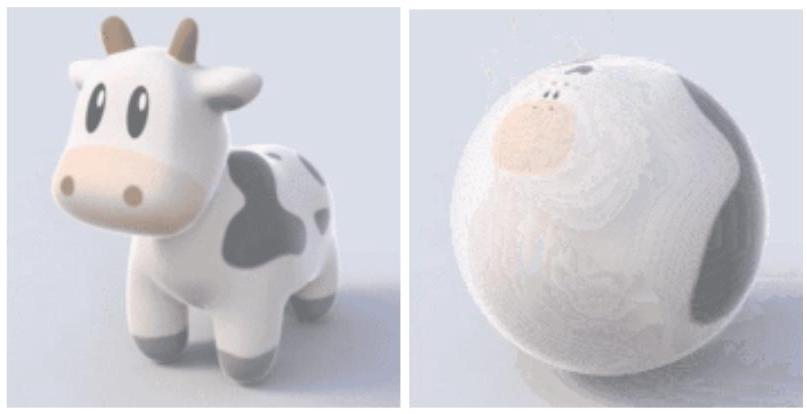
\includegraphics[width=0.5\textwidth]{images/ch1_cow.jpg}
\end{center}
\hspace*{3em} 

Another example is that the coffee cup and the donut have the same topology:

\begin{center}
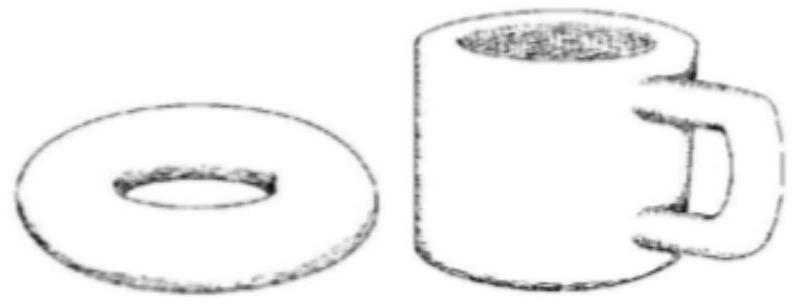
\includegraphics[width=0.5\textwidth]{images/ch1_donutmug.jpg}
\end{center}

However, the two objects below have the intrinsically different topologies:

\begin{center}
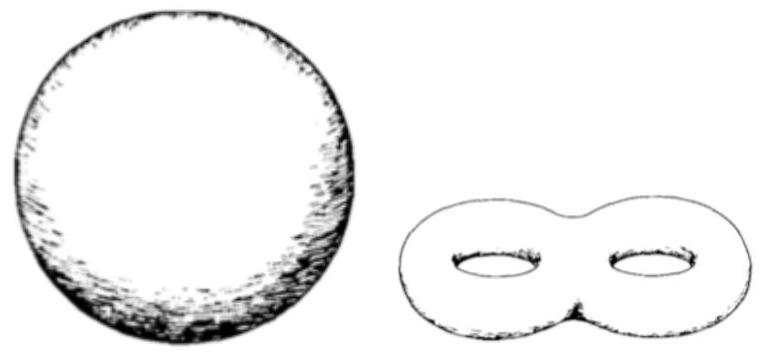
\includegraphics[width=0.5\textwidth]{images/ch1_twoholes.jpg}
\end{center}

In this course, we will study the phenomenon described above mathematically.

\section{Metric Spaces}
In this section, we will study a special kind of topological space.

\begin{definition}[Metric Space] \label{def:metric_space} A metric space \((X,d)\) is a non-empty set endowed with a function (distance function) \(d : X \times  X \rightarrow  \mathbb{R}\) such that

1. \(d\left( {\mathbf{x},\mathbf{y}}\right)  \geq  0\) for \(\forall \mathbf{x},\mathbf{y} \in  X\) with equality iff \(\mathbf{x} = \mathbf{y}\)

2. \(d\left( {\mathbf{x},\mathbf{y}}\right)  = d\left( {\mathbf{y},\mathbf{x}}\right)\)

3. \(d\left( {\mathbf{x},\mathbf{z}}\right)  \leq  d\left( {\mathbf{x},\mathbf{y}}\right)  + d\left( {\mathbf{y},\mathbf{z}}\right)\) (triangle inequality)
\end{definition}

\begin{example} \begin{enumerate}
    \item Let \(X = {\mathbb{R}}^{n}\). Then the distance functions:
\[
{d}_{2}\left( {\mathbf{x},\mathbf{y}}\right)  = \sqrt{\mathop{\sum }\limits_{{i = 1}}^{n}{\left( {x}_{i}- {y}_{i}\right) }^{2}}
\quad, \quad {d}_{\infty }\left( {\mathbf{x},\mathbf{y}}\right)  = \mathop{\max }\limits_{{i = 1,\ldots,n}}\left| {{x}_{i}- {y}_{i}}\right|
\]
define two different metric spaces of the same set $X$.

\item Let \(X\) be any set, and define the discrete metric
\[
d\left( {\mathbf{x},\mathbf{y}}\right)  = \left\{  \begin{array}{ll} 0, & \text{ if }x = y \\  1, & \text{ if }x \neq  y \end{array}\right.
\]
\end{enumerate}
(Homework Show that (1) and (2) defines a metric.)
\end{example}

\begin{definition}[Open Ball] Let $(X,d)$ be a metric space. An open ball of radius \(r\) centered at \(\mathbf{x} \in  X\) is the set
\[
{B}_{r}\left( \mathbf{x}\right)  = \{ \mathbf{y} \in  X \mid  d\left( {\mathbf{x},\mathbf{y}}\right)  < r\}
\]
\end{definition}

\begin{example} \begin{enumerate}
    \item The set \({B}_{1}\left( {0,0}\right)\) defines an open ball under the metric \(\left( {X = {\mathbb{R}}^{2},{d}_{2}}\right)\), or the metric \(\left( {X = {\mathbb{R}}^{2},{d}_{\infty }}\right)\). The corresponding diagram is shown below:
\begin{center}
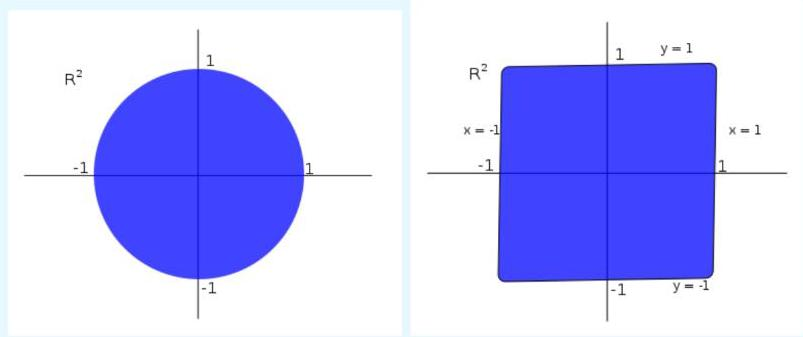
\includegraphics[width=0.6\textwidth]{images/ch1_ball_square.jpg}
\end{center}

\item Under the discrete metric \(({X = {\mathbb{R}}^{2}}, d_{discrete})\), the open ball \({B}_{1}\left( {{\bf x},0}\right)\) is a single point.
\end{enumerate}
\end{example}

\begin{definition}[Open Set] \label{def:open_set} Let \(X\) be a metric space, \(U \subseteq  X\) is an open set in \(X\) if \(\forall u \in  U\), there exists \({\epsilon }_{u} > 0\) such that \({B}_{{\epsilon }_{u}}\left( u\right)  \subseteq  U\).
\end{definition}

Now we get our first taste of topology- the main subject we are studying in this course:
\begin{definition} The \emph{topology} $(X, \mathcal{T})$ induced from a metric space $(X, d)$ is the collection of all open sets 
$$\mathcal{T} := \{ U \subset X\ |\ U\ \text{is open}\}$$ 
in $(X, d)$ (by convention, we decree that the empty set \(\varnothing \in \mathcal{T}\) is open).
\end{definition}

\begin{proposition} All open balls \({B}_{r}\left( \mathbf{x}\right)\) are open in $(X, d)$, i.e. ${B}_{r}\left( \mathbf{x}\right) \in \mathcal{T}$.
\end{proposition}

\begin{proof} Consider the example \(X = \mathbb{R}\) with metric \({d}_{2}\). Therefore \({B}_{r}\left( x\right)  = \left( {x- r,x + r}\right)\). Take \(\mathbf{y} \in  {B}_{r}\left( \mathbf{x}\right)\) such that \(d\left( {\mathbf{x},\mathbf{y}}\right)  = q < r\) and consider \({B}_{\left( {r- q}\right) /2}\left( \mathbf{y}\right)\) : for all \(z \in  {B}_{\left( {r- q}\right) /2}\left( \mathbf{y}\right)\), we have
\[
d\left( {\mathbf{x},\mathbf{z}}\right)  \leq  d\left( {\mathbf{x},\mathbf{y}}\right)  + d\left( {\mathbf{y},\mathbf{z}}\right)  < q + \frac{r- q}{2} < r,
\]
which implies \(z \in  {B}_{r}\left( x\right)\).
\end{proof}

\begin{proposition} \label{prop:open_metric_space} Let $(X, d)$ be a metric space, and \(\mathcal{T}\) is the topology induced from $(X, d)$, then
\begin{enumerate}
    \item Let \(\left\{  {{G}_{\alpha } \mid  \alpha  \in  \mathcal{A}}\right\}\) be such that \({G}_{\alpha } \in  \mathcal{T}\) for all $\alpha \in \mathcal{A}$, then \[\mathop{\bigcup }\limits_{{\alpha  \in  \mathcal{A}}}{G}_{\alpha } \in  \mathcal{T}\].
\item let \({G}_{1},\ldots,{G}_{n} \in  \mathcal{T}\), then 
\[\mathop{\bigcap }\limits_{{i = 1}}^{n}{G}_{i} \in  \mathcal{T}\]
that is, the finite intersection of open sets is open.
\end{enumerate}
\end{proposition}

\begin{proof} \begin{enumerate}
    \item Take \(x \in  \mathop{\bigcup }\limits_{{\alpha  \in  \mathcal{A}}}{G}_{\alpha }\), then \(x \in  {G}_{\beta }\) for some \(\beta  \in  \mathcal{A}\). Since \({G}_{\beta }\) is open, there exists \({\epsilon }_{x} > 0\) such that
\[
{B}_{{\epsilon }_{x}}\left( x\right)  \subseteq  {G}_{\beta } \subseteq  \mathop{\bigcup }\limits_{{\alpha  \in  \mathcal{A}}}{G}_{\alpha }
\]

\item Take \(x \in  \mathop{\bigcap }\limits_{{i = 1}}^{n}{G}_{i}\), i.e., \(x \in  {G}_{i}\) for \(i = 1,\ldots,n\), i.e., there exists \({\epsilon }_{i} > 0\) such that \({B}_{{\epsilon }_{i}}\left( x\right)  \subseteq  {G}_{i}\) for \(i = 1,\ldots,n\). Take \(\epsilon  = \min \left\{  {{\epsilon }_{1},\ldots,{\epsilon }_{n}}\right\}\), which implies
\[
{B}_{\epsilon }\left( x\right)  \subseteq  {B}_{{\epsilon }_{i}}\left( x\right)  \subseteq  {G}_{i},\forall i
\]
which implies \({B}_{\epsilon }\left( x\right)  \subseteq  \mathop{\bigcap }\limits_{{i = 1}}^{n}{G}_{i}\)
\end{enumerate}
\end{proof}

\begin{exercise}
\begin{enumerate}
    \item Let \({\mathcal{T}}_{2},{\mathcal{T}}_{\infty }\) be topologies induced from the metrics \({d}_{2},{d}_{\infty }\) in \({\mathbb{R}}^{2}\). Show that \({\mathcal{T}}_{2} = {\mathcal{T}}_{\infty }\), i.e., every open set in \(\left( {{\mathbb{R}}^{2},{d}_{2}}\right)\) is open in \(\left( {{\mathbb{R}}^{2},{d}_{\infty }}\right)\), and every open set in \(\left( {{\mathbb{R}}^{2},{d}_{\infty }}\right)\) is open in \(\left( {{\mathbb{R}}_{2},{d}_{2}}\right)\).

\item Let \(\mathcal{T}\) be the topology induced from the discrete metric \(\left( {X,{d}_{\text{ discrete }}}\right)\). What is \(\mathcal{T}\)?
\end{enumerate} 
\end{exercise}

({\it Hint:} for (1), show that an open ball in \({d}_{2}\)-metric is open in \({d}_{\infty }\); any open set in \({d}_{2}\)-metric is open in \({d}_{\infty }\); then switch the roles of \({d}_{2}\) and \({d}_{\infty }\)).


\section{Understanding Metric Space by its Topology}
In a standard second course of analysis, one studies various properties of metric spaces $(X,d)$ such as closedness, compactness, continuous maps, etc. In this section, we will re-define these familiar notions by just using the topology $\mathcal{T}$ of $X$.

\subsection{Closed sets}
\begin{definition}[Closed] A subset \(V \subseteq  X\) is closed if \(X \smallsetminus  V\) is open.
\end{definition}

\begin{example} Under the metric space \(\left( {\mathbb{R},{d}_{1}}\right)\),
\[
\mathbb{R} \smallsetminus  \left\lbrack  {b,a}\right\rbrack   = \left( {a,\infty }\right) \bigcup \left( {-\infty,b}\right) \text{ is open } \Rightarrow  \left\lbrack  {b,a}\right\rbrack  \text{ is closed }
\]

1. \(\varnothing,X\) is closed in \(X\)

2. If \({F}_{\alpha }\) is closed in \(X\), so is \(\mathop{\bigcap }\limits_{{\alpha  \in  A}}{F}_{\alpha }\).

3. If \({F}_{1},\ldots,{F}_{k}\) is closed, so is \(\mathop{\bigcup }\limits_{{i = 1}}^{k}{F}_{i}\).
\end{example}

\begin{proof} 1. Note that \(X\) is open in \(X\), which implies \(\varnothing  = X \smallsetminus  X\) is closed in \(X\); Similarly, \(\varnothing\) is open in \(X\), which implies \(X = X \smallsetminus  \varnothing\) is closed in \(X\);

2. The set \({F}_{\alpha }\) is closed implies there exists open \({U}_{\alpha } \subseteq  X\) such that \({F}_{\alpha } = X \smallsetminus  {U}_{\alpha }\). By De Morgan's Law,
\[
\mathop{\bigcap }\limits_{{\alpha  \in  A}}{F}_{\alpha } = \mathop{\bigcap }\limits_{{\alpha  \in  A}}\left( {X \smallsetminus  {U}_{\alpha }}\right)  = X \smallsetminus  \left( {\mathop{\bigcup }\limits_{{\alpha  \in  A}}{U}_{\alpha }}\right).
\]

By part (1) in \autoref{prop:open_metric_space}, the set \(\mathop{\bigcup }\limits_{{\alpha  \in  A}}{U}_{\alpha }\) is open, which implies \(\mathop{\bigcap }\limits_{{\alpha  \in  A}}{F}_{\alpha }\) is closed.

3. The result follows from part (2) in \autoref{prop:open_metric_space} by taking complements. We illustrate examples where open set is used to define convergence and continuity.
\end{proof}

\subsection{Convergence of sequences}
Recall that in the case of metric space $(X, d)$, a sequence of $X$ \(\left\{  {x}_{n}\right\} \rightarrow  x\) converges to $x \in X$ means
\[
\forall \varepsilon  > 0,\exists N\text{ such that }d\left( {{x}_{n},x}\right)  < \varepsilon,\forall n \geq  N\text{. }
\]
We will study the convergence by using $\mathcal{T}$ instead of $d$.

\begin{proposition} Let \((X,d)\) be a metric space, then \(\left\{  {x}_{n}\right\}  \rightarrow  x\) if and only if for \(\forall\) open set \(U \ni  x\), there exists \(N\) such that \({x}_{n} \in  U\) for \(\forall n \geq  N\).
\end{proposition}

\begin{proof} Necessity: Since \(U \ni  x\) is open, there exists \(\varepsilon  > 0\) such that \({B}_{\varepsilon }\left( x\right)  \subseteq  U\).
Since \(\left\{  {x}_{n}\right\}   \rightarrow  x\), there exists \(N\) such that \(d\left( {{x}_{n},x}\right)  < \varepsilon\), i.e., \({x}_{n} \in  {B}_{\varepsilon }\left( x\right)  \subseteq  U\) for \(\forall n \geq  N\).

Sufficiency: Let \(\varepsilon  > 0\) be given. Take the open set \(U = {B}_{\varepsilon }\left( x\right)  \ni  x\), then there exists \(N\)
\end{proof}

\subsection{Continuity}
\begin{definition}[Continuity] Let $(X, d)$ and \(\left( {Y,\rho }\right)\) be given metric spaces. Then \(f : X \rightarrow  Y\) is continuous at \({x}_{0} \in  X\) if
\[
\forall \varepsilon  > 0,\exists \delta  > 0\text{ such that }d\left( {x,{x}_{0}}\right)  < \delta  \Rightarrow  \rho \left( {f\left( x\right),f\left( {x}_{0}\right) }\right)  < \varepsilon \text{. }
\]
The function \(f\) is continuous on \(X\) if \(f\) is continuous for all \({x}_{0} \in  X\).
\end{definition}

As before, we now get rid of metrics to study continuity:
\begin{proposition} \label{prop:metric_cont_map} Let $X, Y$ be metric spaces, and $f:X \to Y$ is a function. 

\begin{enumerate}
    \item The function \(f\) is continuous at \(x\) if and only if for all open \(U \ni  f\left( x\right)\), there exists \(\delta  > 0\) such that the set \(B\left( {x,\delta }\right)  \subseteq  {f}^{-1}\left( U\right)\).

\item The function \(f\) is continuous on \(X\) if and only if \({f}^{-1}\left( U\right)\) is open in \(X\) for each open set \(U \subseteq  Y\).
\end{enumerate}
\end{proposition}

During the proof we will apply a small lemma, whose proof will be left as an exercise to the readers:
\begin{lemma} \label{lem:metric_cont_map} \(f\) is continuous at \(x\) if and only if for all \(\left\{  {x}_{n}\right\}   \rightarrow  x\), we have \(\left\{  {f\left( {x}_{n}\right) }\right\}   \rightarrow  f\left( x\right)\).
\end{lemma}

\begin{proof} \begin{enumerate}
    \item Necessity: Due to the openness of \(U \ni  f\left( x\right)\), there exists a ball \(B\left( {f\left( x\right),\varepsilon }\right)  \subseteq  U\). Due to the continuity of \(f\) at \(x\), there exists \(\delta  > 0\) such that \(d\left( {x,{x}^{\prime }}\right)  < \delta\) implies \(d\left( {f\left( x\right),f\left( {x}^{\prime }\right) }\right)  < \varepsilon\), which implies:
\[
f\left( {B\left( {x,\delta }\right) }\right)  \subseteq  B\left( {f\left( x\right),\varepsilon }\right)  \subseteq  U,
\]
and hence \(B\left( {x,\delta }\right)  \subseteq  {f}^{-1}\left( U\right)\).

Sufficiency: Let \(\left\{  {x}_{n}\right\} \rightarrow  x\). By \autoref{lem:metric_cont_map}, it suffices to show \(\left\{  {f\left( {x}_{n}\right) }\right\}   \rightarrow  f\left( x\right)\). 

By hypothesis, for each open \(U \ni  f\left( x\right)\), there exists \(\delta  > 0\) such that \({B}_{\delta }\left( x\right)  \subseteq  {f}^{-1}\left( U\right)\). Since \(\left\{  {x}_{n}\right\}   \rightarrow  x\), there exists \(N\) such that
\[
{x}_{n} \in  {B}_{\delta }\left( x\right)  \subseteq  {f}^{-1}\left( U\right),\forall n \geq  N \Rightarrow  f\left( {x}_{n}\right)  \in  U,\forall n \geq  N
\]
We now show that $f$ is continuous in the conventional sense - let \(\varepsilon  > 0\) be given, and then construct the \(U = {B}_{\varepsilon }\left( {f\left( x\right) }\right)\). The argument above shows that \(f\left( {x}_{n}\right)  \in  {B}_{\varepsilon }\left( {f\left( x\right) }\right)\) for \(\forall n \geq  N\), which implies \(\rho \left( {f\left( {x}_{n}\right),f\left( x\right) }\right)  < \varepsilon\), i.e., \(\left\{  {f\left( {x}_{n}\right) }\right\}   \rightarrow  f\left( x\right)\).

\item For the forward direction, it suffices to show that each point \(x\) of \({f}^{-1}\left( U\right)\) is an interior point of \({f}^{-1}\left( U\right)\), which is shown by (1); the converse follows trivially by applying (1).
\end{enumerate}
\end{proof}


As illustrated above, convergence, continuity, (and compactness) can be defined by using open sets \(\mathcal{T}\) only.

\chapter{Topological Spaces}

Definition 1.21 A topological space(X, T)consists of a (non-empty) set \(X\) , and a family of subsets of \(X\) ("open sets" \(\mathcal{T}\) ) such that

1. \(\varnothing ,X \in  \mathcal{T}\)

2. \(U,V \in  \mathcal{T}\) implies \(U \cap  V \in  \mathcal{T}\)

3. If \({U}_{\alpha } \in  \mathcal{T}\) for all \(\alpha  \in  \mathcal{A}\) , then \(\mathop{\bigcup }\limits_{{\alpha  \in  \mathcal{A}}}{U}_{\alpha } \in  \mathcal{T}\) .

The elements in \(\mathcal{T}\) are called open subsets of \(X\) . The \(\mathcal{T}\) is called a topology on \(X\) .

1. Let(X, d)be any metric space, and

\[
\mathcal{T} = \{ \text{ all open subsets of }X\}
\]

It’s clear that \(\mathcal{T}\) is a topology on \(X\) .

\section*{2. Define the discrete topology}

\[
{\mathcal{T}}_{\text{ dis }} = \{ \text{ all subsets of }X\}
\]

It’s clear that \({\mathcal{T}}_{\text{ dis }}\) is a topology on \(X\) ,(which also comes from the discrete metric \(\left( {X,{d}_{\text{ discrete }}}\right)\) ).

R) We say(X, T)is induced from a metric(X, d)(or it is metrizable) if \(\mathcal{T}\) is the faimly of open subsets in(X, d).

3. Consider the indiscrete topology \(\left( {X,{\mathcal{T}}_{\text{ indis }}}\right)\) , where \(X\) contains more than one element:

\[
{\mathcal{T}}_{\text{ indis }} = \{ \varnothing ,X\} \text{ . }
\]

Question: is \(\left( {X,{\mathcal{T}}_{\text{ indis }}}\right)\) metrizable? No. For any metric \(d\) defined on \(X\) , let \(x,y\) be distinct points in \(X\) , and then \(\varepsilon  \mathrel{\text{ := }} d\left( {x,y}\right)  > 0\) , hence \({B}_{\frac{1}{2}\varepsilon }\left( x\right)\) is a open set belonging to the corresponding induced topology. Since \(x \in  {B}_{\frac{1}{2}\varepsilon }\left( x\right)\) and \(y \notin  {B}_{\frac{1}{2}\varepsilon }\left( y\right)\) , we conclude that \({B}_{\frac{1}{2}\varepsilon }\left( x\right)\) is neither \(\varnothing\) nor \(X\) , i.e., the topology induced by any metric \(d\) is not the indiscrete topology.

4. Consider the cofinite topology \(\left( {X,{\mathcal{T}}_{\text{ cofin }}}\right)\) :

\[
{\mathcal{T}}_{\text{ cofin }} = \{ U \mid  X \smallsetminus  U\text{ is a finite set }\} \bigcup \{ \varnothing \}
\]

Question: is \(\left( {X,{\mathcal{T}}_{\text{ cofin }}}\right)\) metrizable?

Definition 1.22 [Equivalence] Two metric spaces are topologically equivalent if they give rise to the same topology.

\begin{itemize}
\item Example 1.21 Metrics \({d}_{1},{d}_{2},{d}_{\infty }\) in \({\mathbb{R}}^{n}\) are topologically equivalent.
\end{itemize}

\section*{1.6.3. Closed Subsets}

Definition 1.23 [Closed] Let(X, T)be a topology space. Then \(V \subseteq  X\) is closed if \(X \smallsetminus  V \in  \mathcal{T}\)

\begin{itemize}
\item Example 1.22 Under the topology space \(\left( {\mathbb{R},{\mathcal{T}}_{\text{ usual }}}\right) ,\left( {b,\infty }\right)  \cup  \left( {-\infty ,a}\right)  \in  \mathcal{T}\) . Therefore,
\end{itemize}

\[
\left\lbrack  {a,b}\right\rbrack   = \mathbb{R} \smallsetminus  \left( {\left( {b,\infty }\right) \bigcup \left( {-\infty ,a}\right) }\right)
\]

is closed in \(\mathbb{R}\) under usual topology.

It is important to say that \(V\) is closed in \(X\) . You need to specify the underlying the space \(X\) .

\section*{2.3. Monday for MAT4002}

\section*{Reviewing.}

1. Topological Space(X, J): a special class of topological space is that induced from metric space(X, d):

(X, T), with \(\mathcal{T} = \{\) all open sets in \(\left( {X,d}\right) \}\)

2. Closed Sets \(\left( {X \smallsetminus  U}\right)\) with \(U\) open.

Proposition 2.8 Let(X, T)be a topological space,

1. \(\varnothing ,X\) are closed in \(X\)

2. \({V}_{1},{V}_{2}\) closed in \(X\) implies that \({V}_{1} \cup  {V}_{2}\) closed in \(X\)

3. \(\left\{  {{V}_{\alpha } \mid  \alpha  \in  \mathcal{A}}\right\}\) closed in \(X\) implies that \(\mathop{\bigcap }\limits_{{\alpha  \in  \mathcal{A}}}{V}_{\alpha }\) closed in \(X\)

Proof. Applying the De Morgan's Law

\(\left( {X \smallsetminus  \mathop{\bigcup }\limits_{{i \in  I}}{U}_{i}}\right)  = \mathop{\bigcap }\limits_{{i \in  I}}\left( {X \smallsetminus  {U}_{i}}\right)\)

\section*{2.3.1. Convergence in topological space}

Definition 2.4 [Convergence] A sequence \(\left\{  {x}_{n}\right\}\) of a topological space(X, T)converges to \(x \in  X\) if \(\forall U \ni  x\) is open, there \(\exists N\) such that \({x}_{n} \in  U,\forall n \geq  N\) .

Example 2.9 1. The topology for the space \(\left( {X = {\mathbb{R}}^{n},{d}_{2}}\right)  \rightarrow  \left( {X,\mathcal{T}}\right)\) (i.e., a topological space induced from meric space \(\left( {X = {\mathbb{R}}^{n},{d}_{2}}\right)\) is called a usual topology on \({\mathbb{R}}^{n}\) .

When I say \({\mathbb{R}}^{n}\) (or subset of \({\mathbb{R}}^{n}\) ) is a topological space, it is equipeed with usual topology.

Convergence of sequence in \(\left( {{\mathbb{R}}^{n},\mathcal{T}}\right)\) is the usual convergence in analysis.

For \({\mathbb{R}}^{n}\) or metric space, the limit of sequence (if exists) is unique.

2. Consider the topological space \(\left( {X,{\mathcal{T}}_{\text{ indiscrete }}}\right)\) . Take any sequence \(\left\{  {x}_{n}\right\}\) in \(X\) , it is convergent to any \(x \in  X\) . Indeed, for \(\forall U \ni  x\) open, \(U = X\) . Therefore,

\[
{x}_{n} \in  U\left( { = X}\right) ,\forall n \geq  1\text{ . }
\]

3. Consider the topological space \(\left( {X,{\mathcal{T}}_{\text{ cofinite }}}\right)\) , where \(X\) is infinite. Consider \(\left\{  {x}_{n}\right\}\) is a sequence satisfying \(m \neq  n\) implies \({x}_{m} \neq  {x}_{n}\) . Then \(\left\{  {x}_{n}\right\}\) is convergent to any \(x \in  X\) . (Question: how to define openness for \({\mathcal{T}}_{\text{ cofinite }}\) and \({\mathcal{T}}_{\text{ indiscrete }}\) )?

4. Consider the topological space \(\left( {X,{\mathcal{T}}_{\text{ discrete }}}\right)\) , the sequence \(\left\{  {x}_{n}\right\}   \rightarrow  x\) is equivalent to say \({x}_{n} = x\) for all sufficiently large \(n\) .

The limit of sequences may not be unique. The reason is that " \(\mathcal{T}\) is not big enough". We will give a criterion to make sure the limit is unique in the future. (Hausdorff)

Proposition 2.9 If \(F \subseteq  \left( {X,\mathcal{T}}\right)\) is closed, then for any convergent sequence \(\left\{  {x}_{n}\right\}\) in \(F\) , the limit(s) are also in \(F\) .

Proof. Let \(\left\{  {x}_{n}\right\}\) be a sequence in \(F\) with limit \(x \in  X\) . Suppose on the contrary that \(x \notin  F\) (i.e., \(x \in  X \smallsetminus  F\) that is open). There exists \(N\) such that

\[
{x}_{n} \in  X \smallsetminus  F,\forall n \geq  N
\]

i.e., \({x}_{n} \notin  F\) , which is a contradiction.

The converse may not be true. If the(X, T)is metrizable, the converse holds. Counter-example: Consider the co-countable topological space \(\left( {X = \mathbb{R},{\mathcal{T}}_{\text{ co-co }}}\right)\) , where

\[
{\mathcal{T}}_{\mathrm{{co}}\text{ -co }} = \{ U \mid  X \smallsetminus  U\text{ is a countable set }\} \bigcup \{ \varnothing \} ,
\]

and \(X\) is uncontable. Then note that \(F = \left\lbrack  {0,1}\right\rbrack   \subsetneqq  X\) is an un-countable set, and under co-countable topology, \(F \supseteq  \left\{  {x}_{n}\right\}   \rightarrow  x\) implies \({x}_{n} = x \in  F\) for all \(n\) . It’s clear that \(X \smallsetminus  F \notin  {\mathcal{T}}_{\mathrm{{co}} - \mathrm{{co}}}\) , i.e., \(F\) is not closed.

\section*{2.3.2. Interior, Closure, Boundary}

Definition 2.5 Let(X, T)be a topological space, and \(A \subseteq  X\) a subset.

1. The interior of \(A\) is

\[
{A}^{ \circ  } = \mathop{\bigcup }\limits_{{U \subseteq  A,U\text{ is open }}}U
\]

2. The closure of \(A\) is

\[
\bar{A} = \mathop{\bigcap }\limits_{{A \subseteq  V,V\text{ is closed }}}V
\]

If \(\bar{A} = X\) , we say that \(A\) is dense in \(X\) .

The graph illustration of the definition above is as follows:

\begin{center}
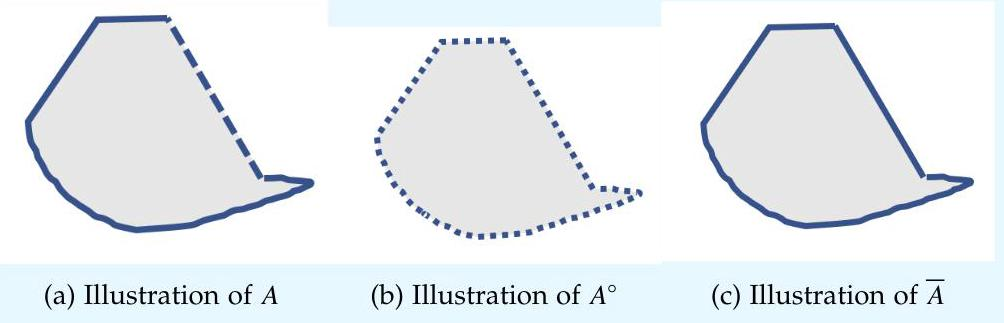
\includegraphics[max width=0.8\textwidth]{images/bo_d2bcsrref24c73avs720_25_282_922_1004_323_0.jpg}
\end{center}
\hspace*{3em} 

Figure 2.1: Graph Illustrations

\begin{itemize}
\item Example 2.10 1. For \(\lbrack a,b) \subseteq  \mathbb{R}\) , we have:
\end{itemize}

\[
\lbrack a,b{)}^{ \circ  } = \left( {a,b}\right) ,\;\overline{\lbrack a,b)} = \left\lbrack  {a,b}\right\rbrack
\]

2. For \(X = \mathbb{R},{\mathbb{Q}}^{ \circ  } = \varnothing\) and \(\overline{\mathbb{Q}} = \mathbb{R}\) .

3. Consider the discrete topology \(\left( {X,{\mathcal{T}}_{\text{ discrete }}}\right)\) , we have

\[
{S}^{ \circ  } = S,\;\bar{S} = S
\]

The insights behind the definition (2.5) is as follows

Proposition 2.10 1. \({A}^{ \circ  }\) is the largest open subset of \(X\) contained in \(A\) ;

\(\bar{A}\) is the smallest closed subset of \(X\) containing \(A\) .

2. If \(A \subseteq  B\) , then \({A}^{ \circ  } \subseteq  B\) and \(\bar{A} \subseteq  \bar{B}\)

3. \(A\) is open in \(X\) is equivalent to say \({A}^{ \circ  } = A;A\) is closed in \(X\) is equivalent to say \(\bar{A} = A\) .

\begin{itemize}
\item Example 2.11 Let(X, d)be a metric space. What’s the closure of an open ball \({B}_{r}\left( x\right)\) ? The direct intuition is to define the closed ball
\end{itemize}

\[
{\bar{B}}_{r}\left( x\right)  = \{ y \in  X \mid  d\left( {x,y}\right)  \leq  r\} .
\]

Question: is \({\bar{B}}_{r}\left( x\right)  = \overline{{B}_{r}\left( x\right) }\) ?

1. Since \({\bar{B}}_{r}\left( x\right)\) is a closed subset of \(X\) , and \({B}_{r}\left( x\right)  \subseteq  {\bar{B}}_{r}\left( x\right)\) , we imply that

\[
\overline{{B}_{r}\left( x\right) } \subseteq  {\bar{B}}_{r}\left( x\right)
\]

2. Howover, we may find an example such that \(\overline{{B}_{r}\left( x\right) }\) is a proper subset of \({\bar{B}}_{r}\left( x\right)\) : Consider the discrete metric space \(\left( {X,{d}_{\text{ discrete }}}\right)\) and for \(\forall x \in  X\) ,

\[
{B}_{1}\left( x\right)  = \{ x\}  \Rightarrow  \overline{{B}_{1}\left( x\right) } = \{ x\} ,\;{\bar{B}}_{1}\left( x\right)  = X
\]

The equality \({\bar{B}}_{r}\left( x\right)  = \overline{{B}_{r}\left( x\right) }\) holds when(X, d)is a normed space. Here is another characterization of \(\bar{A}\) : Proposition 2.11

\[
\bar{A} = \{ x \in  X \mid  \forall \text{ open }U \ni  x,U\bigcap A \neq  \varnothing \}
\]

Proof. Define

\[
S = \{ x \in  X \mid  \forall \text{ open }U \ni  x,U \cap  A \neq  \varnothing \}
\]

It suffices to show that \(\bar{A} = S\) . 1. First show that \(S\) is closed:

\[
X \smallsetminus  S = \left\{  {x \in  X\mid \exists {U}_{x} \ni  x\text{ open s.t. }{U}_{x} \cap  A = \varnothing }\right\}
\]

Take \(x \in  X \smallsetminus  S\) , we imply there exists open \({U}_{x} \ni  x\) such that \({U}_{x} \cap  A = \varnothing\) . We claim

\({U}_{x} \subseteq  X \smallsetminus  S\)

\begin{itemize}
\item For \(\forall y \in  {U}_{x}\) , note that \({U}_{x} \ni  y\) that is open, such that \({U}_{x} \cap  A = \varnothing\) . Therefore,
\end{itemize}

\(y \in  X \smallsetminus  S\) .

Therefore, we have \(x \in  {U}_{x} \subseteq  X \smallsetminus  S\) for any \(\forall x \in  X \smallsetminus  S\) .

Note that

\[
X \smallsetminus  S = \mathop{\bigcup }\limits_{{x \in  X \smallsetminus  S}}\{ x\}  \subseteq  \mathop{\bigcup }\limits_{{x \in  X \smallsetminus  S}}{U}_{x} \subseteq  X \smallsetminus  S,
\]

which implies \(X \smallsetminus  S = \mathop{\bigcup }\limits_{{x \in  X \smallsetminus  S}}{U}_{x}\) is open, i.e., \(S\) is closed in \(X\) .

2. By definition, it is clear that \(A \subseteq  S\) :

\[
\forall a \in  A,\forall \text{ open }U \ni  a,U\bigcap A \supseteq  \{ a\}  \neq  \varnothing  \Rightarrow  a \in  S.
\]

Therefore, \(\bar{A} \subseteq  \bar{S} = S\) .

3. Suppose on the contrary that there exists \(y \in  S \smallsetminus  \bar{A}\) .

Since \(y \notin  \bar{A}\) , by definition, there exists \(F \supseteq  A\) closed such that \(y \notin  F\) .

Therefore, \(y \in  X \smallsetminus  F\) that is open, and

\[
\left( {X \smallsetminus  F}\right) \bigcap A \subseteq  \left( {X \smallsetminus  A}\right) \bigcap A = \varnothing  \Rightarrow  y \notin  S,
\]

which is a contradiction. Therefore, \(S = \bar{A}\) .

Definition 2.6 [accumulation point] Let \(A \subseteq  X\) be a subset in a topological space. We call \(x \in  X\) are an accumulation point (limit point) of \(A\) if

\[
\forall U \subseteq  X\text{ open s.t. }U \ni  x,\left( {U\smallsetminus \{ x\} }\right) \bigcap A \neq  \varnothing .
\]

Proposition \({2.12}\;\bar{A} = A\bigcup {A}^{\prime }\) .

Proof. This proposition directly follows from Proposition (2.11) and the definition of \({\mathrm{A}}^{\prime }\) .

\section*{2.6. Wednesday for MAT4002}

Reviewing.

1. Interior, Closure:

\[
\bar{A} = \{ x \mid  \forall U \ni  x\text{ open },U\bigcap A \neq  \varnothing \}
\]

2. Accumulation points

\section*{2.6.1. Remark on Closure}

Definition 2.14 [Sequential Closure] Let \({A}_{S}\) be the set of limits of any convergent sequence in \(A\) , then \({A}_{S}\) is called the sequential closure of \(A\) .

Definition 2.15 [Accumulation/Cluster Points] The set of accumulation (limit) points is defined as

\[
{A}^{\prime } = \{ x \mid  \forall U \ni  x\text{ open },\left( {U\smallsetminus \{ x\} }\right) \bigcap A \neq  \varnothing \}
\]

®

1. (a) There exists some point in \(A\) but not in \({A}^{\prime }\) :

\[
A = \{ 1,2,3,\ldots ,n,\ldots \}
\]

Then any point in \(A\) is not in \({A}^{\prime }\)

(b) There also exists some point in \({A}^{\prime }\) but not in \(A\) :

\[
A = \left\{  {\left. \frac{1}{n}\right| \;n \geq  1}\right\}
\]

Then the point 0 is in \({A}^{\prime }\) but not in \(A\) .

2. The closure \(\bar{A} = A \cup  {A}^{\prime }\) .

3. The size of the sequentical closure \({A}_{S}\) is between \(A\) and \(\bar{A}\) , i.e., \(A \subseteq  {A}_{S} \subseteq  \bar{A}\) : It’s clear that \(A \subseteq  {A}_{S}\) , since the sequence \(\left\{  {{a}_{n} \mathrel{\text{ := }} a}\right\}\) is convergent to \(a\) for

\(\forall a \in  A\) .

For all \(a \in  {A}_{S}\) , we have \(\left\{  {a}_{n}\right\}   \rightarrow  a\) . Then for any open \(U \ni  a\) , there exists

\(N\) such that \(\left\{  {{a}_{N},{a}_{N + 1},\ldots }\right\}   \subseteq  U \cap  A \neq  \varnothing\) . Therefore, \(a \in  \bar{A}\) , i.e., \({A}_{S} \subseteq  \bar{A}\) .

Question: Is \({A}_{S} = \bar{A}\) ?

Proposition 2.21 Let(X, d)be a metric space, then \({A}_{S} = \bar{A}\) .

Proof. Let \(a \in  \bar{A}\) , then there exists \({a}_{n} \in  {B}_{1/n}\left( a\right)  \cap  A\) , which implies \(\left\{  {a}_{n}\right\}   \rightarrow  a\) , i.e., \(a \in\)  \({A}_{S}\) .

If(X, T)is metrizable, then \({A}_{S} = \bar{A}\) . The same goes for first countable topological spaces. However, \({A}_{S}\) is a proper subset of \(\bar{A}\) in general:

Let \(A \subseteq  X\) be the set of continuous functions, where \(X = {\mathbb{R}}^{\mathbb{R}}\) denotes the set of all real-valued functions on \(\mathbb{R}\) , with the topology of pointwise convergence.

Then \({A}_{S} = {B}_{1}\) , the set of all functions of first Baire-Category on \(\mathbb{R}\) ; and \({\left\lbrack  {A}_{S}\right\rbrack  }_{S} = {B}_{2}\) , the set of all functions of second Baire-Category on \(\mathbb{R}\) . Since \({B}_{1} \neq  {B}_{2}\) , we have \({\left\lbrack  {A}_{S}\right\rbrack  }_{S} = {A}_{S}\) . Note that \(\overline{\bar{A}} = \bar{A}\) . We conclude that \({A}_{S}\) cannot equal to \(\bar{A}\) , since the sequential closure operator cannot be idemotenet.

Definition 2.16 [Boundary] The boundary of \(\mathbf{A}\) is defined as

\[
\partial \mathbf{A} = \bar{A} \smallsetminus  {A}^{ \circ  }
\]

Proposition 2.22 Let(X, T)be a topological space with \(A,B \subseteq  X\) .

\[
\overline{X \smallsetminus  A} = X \smallsetminus  {A}^{ \circ  },\;{\left( X \smallsetminus  B\right) }^{ \circ  } = X \smallsetminus  \bar{B}\;\partial A = \bar{A} \cap  \left( \overline{X \smallsetminus  A}\right)
\]

Proof.

\[
X \smallsetminus  {A}^{ \circ  } = X \smallsetminus  \left( {\mathop{\bigcup }\limits_{{U\text{ is open, }U \subseteq  A}}U}\right)  \tag{2.2a}
\]

\[
= \mathop{\bigcap }\limits_{{U\text{ is open, }U \subseteq  A}}\left( {X \smallsetminus  U}\right)  \tag{2.2b}
\]

\[
= \mathop{\bigcap }\limits_{{V\text{ is closed, }F \supseteq  X \smallsetminus  A}}F \tag{2.2c}
\]

\[
= \overline{X \smallsetminus  A} \tag{2.2d}
\]

Denoting \(X \smallsetminus  A\) by \(B\) , we obtain:

\[
{\left( X \smallsetminus  B\right) }^{ \circ  } = {A}^{ \circ  } \tag{2.3a}
\]

\[
= X \smallsetminus  \left( {X \smallsetminus  {A}^{ \circ  }}\right)  \tag{2.3b}
\]

\[
= X \smallsetminus  \overline{X \smallsetminus  A} \tag{2.3c}
\]

\[
= X \smallsetminus  \bar{B} \tag{2.3d}
\]

By definition of \(\partial A\) ,

\[
\partial A = \bar{A} \smallsetminus  {A}^{ \circ  } \tag{2.4a}
\]

\[
= \bar{A}\bigcap \left( {X \smallsetminus  {A}^{ \circ  }}\right)  \tag{2.4b}
\]

\[
= \bar{A}\bigcap \left( \overline{X \smallsetminus  A}\right)  \tag{2.4c}
\]

\section*{2.6.2. Functions on Topological Space}

Definition 2.17 [Continuous] Let \(f : \left( {X,{\mathcal{T}}_{X}}\right)  \rightarrow  \left( {Y,{\mathcal{T}}_{Y}}\right)\) be a map. Then the function \(f\) is continuous, if

\[
U \in  {\mathcal{T}}_{Y} \Rightarrow  {f}^{-1}\left( U\right)  \in  {\mathcal{T}}_{X}
\]

1. The identity map id : \(\left( {X,\mathcal{T}}\right)  \rightarrow  \left( {X,\mathcal{T}}\right)\) defined as \(x \mapsto  x\) is continuous

2. The identity map id : \(\left( {X,{\mathcal{T}}_{\text{ discrete }}}\right)  \rightarrow  \left( {X,{\mathcal{T}}_{\text{ indiscrete }}}\right)\) defined as \(x \mapsto  x\) is continuous. Since \({\operatorname{id}}^{-1}\left( \varnothing \right)  = \varnothing\) and \({\operatorname{id}}^{-1}\left( X\right)  = X\)

3. The identity map id : \(\left( {X,{\mathcal{T}}_{\text{ indiscrete }}}\right)  \rightarrow  \left( {X,{\mathcal{T}}_{\text{ discrete }}}\right)\) defined as \(x \mapsto  x\) is not continuous.

Proposition 2.23 If \(f : X \rightarrow  Y\) , and \(g : Y \rightarrow  Z\) be continuous, then \(g \circ  f\) is continuous

Proof. For given \(U \in  {\mathcal{T}}_{Z}\) , we imply

\[
{g}^{-1}\left( U\right)  \in  {\mathcal{T}}_{Y} \Rightarrow  {f}^{-1}\left( {{g}^{-1}\left( U\right) }\right)  \in  {\mathcal{T}}_{X},
\]

i.e., \({\left( g \circ  f\right) }^{-1}\left( U\right)  \in  {\mathcal{T}}_{X}\)

Proposition 2.24 Suppose \(f : X \rightarrow  Y\) is continuous between two topological spaces. Then \(\left\{  {x}_{n}\right\}   \rightarrow  x\) implies \(\left\{  {f\left( {x}_{n}\right) }\right\}   \rightarrow  f\left( x\right)\) .

Proof. Take open \(U \ni  f\left( x\right)\) , which implies \({f}^{-1}\left( U\right)  \ni  x\) . Since \({f}^{-1}\left( U\right)\) is open, we imply there exists \(N\) such that

\[
\left\{  {{x}_{n} \mid  n \geq  N}\right\}   \subseteq  {f}^{-1}\left( U\right)
\]

i.e., \(\left\{  {f\left( {x}_{n}\right)  \mid  n \geq  N}\right\}   \subseteq  U\)

We use the notion of Homeomorphism to describe the equivalence between two topological spaces.

Definition 2.18 [Homeomorphism] A homeomorphism between spaces topological spaces \(\left( {X,{\mathcal{T}}_{X}}\right)\) and \(\left( {Y,{\mathcal{T}}_{Y}}\right)\) is a bijection

\[
f : \left( {X,{\mathcal{T}}_{X}}\right)  \rightarrow  \left( {Y,{\mathcal{T}}_{Y}}\right)
\]

such that both \(f\) and \({f}^{-1}\) are continuous.

\section*{2.6.3. Subspace Topology}

Definition 2.19 Let \(A \subseteq  X\) be a non-empty set. The subspace topology of \(A\) is defined as:

1. \({\mathcal{T}}_{A} \mathrel{\text{ := }} \left\{  {U \cap  A \mid  U \in  {\mathcal{T}}_{A}}\right\}\)

2. The coarsest topology on \(A\) such that the inclusion map

\[
i : \left( {A,{\mathcal{T}}_{A}}\right)  \rightarrow  \left( {X,{\mathcal{T}}_{X}}\right) ,\;i\left( x\right)  = x
\]

is continuous.

(We say the topology \({\mathcal{T}}_{1}\) is coarser than \({\mathcal{T}}_{2}\) , or \({\mathcal{T}}_{2}\) is finer than \({\mathcal{T}}_{1}\) , if \({\mathcal{T}}_{1} \subseteq  {\mathcal{T}}_{2}\)

e.g., \({\mathcal{T}}_{\text{ discrete }}\) is the finest topology, and \({\mathcal{T}}_{\text{ indiscrete }}\) is coarsest topology.)

3. The (unique) topology such that for any \(\left( {Y,{\mathcal{T}}_{Y}}\right)\) ,

\[
f : \left( {Y,{\mathcal{T}}_{Y}}\right)  \rightarrow  \left( {A,{\mathcal{T}}_{A}}\right)
\]

is continuous iff \(i \circ  f : \left( {Y,{\mathcal{T}}_{Y}}\right)  \rightarrow  \left( {X,{\mathcal{T}}_{X}}\right)\) (where \(i\) is the inclusion map) is continuous.

Proposition 2.25 The definition (1) and (2) in (2.19) are equivalent.

Outline. The proof is by applying

\[
{i}^{-1}\left( S\right)  = S\bigcap A,\;\forall S
\]

\begin{itemize}
\item Example 2.17 Let all English and numerical letters be subset of \({\mathbb{R}}^{2}\) : P, 6
\end{itemize}

The homeomorphism can be constrcuted between these two English letters.

Proposition 2.26 The definition (2) and (3) in (2.19) are equivalent.

Proof. Necessity.

\begin{itemize}
\item For \(\forall U \in  {\mathcal{T}}_{X}\) , consider that
\end{itemize}

\[
{\left( i \circ  f\right) }^{-1}\left( U\right)  = {f}^{-1}\left( {{i}^{-1}\left( U\right) }\right)  = {f}^{-1}\left( {U \cap  A}\right)
\]

since \(U \cap  A \in  {\mathcal{T}}_{A}\) and \(f\) is continuous, we imply \({\left( i \circ  f\right) }^{-1}\left( U\right)  \in  {\mathcal{T}}_{Y}\)

\begin{itemize}
\item For \(\forall {U}^{\prime } \in  {\mathcal{T}}_{A}\) , we have \({U}^{\prime } = U \cap  A\) for some \(U \in  {\mathcal{T}}_{X}\) . Therefore,
\end{itemize}

\[
{f}^{-1}\left( {U}^{\prime }\right)  = {f}^{-1}\left( {U \cap  A}\right)  = {f}^{-1}\left( {{i}^{-1}\left( U\right) }\right)  = {\left( i \circ  f\right) }^{-1}\left( U\right)  \in  {\mathcal{T}}_{Y}.
\]

The sufficiency is left as exercise.

Proposition 2.27 1. The definition (1) in (2.19) does define a topology of \(A\)

2. Closed sets of \(A\) under subspace topology are of the form \(V \cap  A\) , where \(V\) is closed in \(X\)

Proposition 2.28 Suppose \(\left( {A,{\mathcal{T}}_{A}}\right)  \subseteq  \left( {X,{\mathcal{T}}_{X}}\right)\) is a subspace topology, and \(B \subseteq  A \subseteq  X\) . Then

1. \({\bar{B}}^{A} = {\bar{B}}^{X} \cap  A\) .

2. \({B}^{\circ A} \supseteq  {B}^{\circ X}\)

Proof. By proposition (2.27), \({\bar{B}}^{X} \cap  A\) is closed in \(A\) , and \({\bar{B}}^{X} \cap  A \supset  B\) , which implies

\[
{\bar{B}}^{A} \subseteq  {\bar{B}}^{X}\bigcap A
\]

Note that \({\bar{B}}^{A} \supset  B\) is closed in \(A\) , which implies \({\bar{B}}^{A} = V \cap  A \subseteq  V\) , where \(V\) is closed in \(X\) . Therefore,

\[
{\bar{B}}^{X} \subseteq  V \Rightarrow  {\bar{B}}^{X} \cap  A \subseteq  V \cap  A = {\bar{B}}^{A}
\]

Therefore, \({\bar{B}}^{A} = {\bar{B}}^{X} \subseteq  V\)

Can we have \({B}^{\circ X} = {B}^{\circ A}\) ?

\section*{2.6.4. Basis (Base) of a topology}

Roughly speaking, a basis of a topology is a family of "generators" of the topology.

Definition 2.20 Let(X, T)be a topological space. A family of subsets \(\mathcal{B}\) in \(X\) is a basis for \(\mathcal{T}\) if

1. \(\mathcal{B} \subseteq  \mathcal{T}\) , i.e., everything in \(\mathcal{B}\) is open

2. Every \(U \in  \mathcal{T}\) can be written as union of elements in \(\mathcal{B}\) .

\begin{itemize}
\item Example 2.18 1. \(\mathcal{B} = \mathcal{T}\) is a basis.
\end{itemize}

2. For \(X = {\mathbb{R}}^{n}\) ,

\[
\mathcal{B} = \left\{  {{B}_{r}\left( \mathbf{x}\right)  \mid  \mathbf{x} \in  {\mathbb{Q}}^{n},r \in  \mathbb{Q}\bigcap \left( {0,\infty }\right) }\right\}
\]

Exercise: every \(\left( {a,b}\right)  = \mathop{\bigcup }\limits_{{i \in  I}}\left( {{p}_{i},{q}_{i}}\right)\) for \({p}_{i},{q}_{i} \in  \mathbb{Q}\) .

Therefore, \(\mathcal{B}\) is countable.

Proposition 2.29 If(X, T)has a countable basis, e.g., \({\mathbb{R}}^{n}\) , then(X, T)has a second-countable space.

\section*{3.3. Monday for MAT4002}

\section*{3.3.1. Remarks on Basis and Homeomorphism}

Reviewing.

1. \(A \subseteq  {A}_{S} \subseteq  \bar{A}\) , where \({A}_{S}\) is sequential closure and \(\bar{A}\) denotes closure.

2. Subspace topology.

3. Homeomorphism. Consider the mapping \(f : X \rightarrow  Y\) with the topogical space

\(X,Y\) shown below, with the standard topology, the question is whether \(f\) is continuous?

\begin{center}
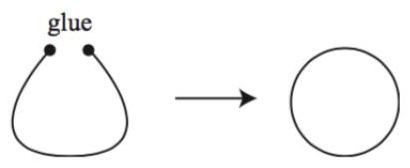
\includegraphics[max width=0.3\textwidth]{images/bo_d2bcsrref24c73avs720_36_777_903_410_168_0.jpg}
\end{center}
\hspace*{3em} 

Figure 3.1: Diagram for mapping \(f\)

The answer is no, since the left in (3.1) can be isomorphically mapped into(0,1); the right can be isomorphically mapped into \(\left\lbrack  {0,1}\right\rbrack\) , and the mapping \(\left( {0,1}\right)  \rightarrow  \left\lbrack  {0,1}\right\rbrack\) cannot be isomorphism:

Proof. Assume otherwise the mapping \(g : \left( {0,1}\right)  \rightarrow  \left\lbrack  {0,1}\right\rbrack\) is isomorphism, and therefore \({f}^{-1}\left( U\right)\) is open for any open set \(U\) in the space \(\left\lbrack  {0,1}\right\rbrack\) .

Construct \(U = (1 - \delta ,1\rbrack\) for \(\delta  \leq  1\) , and therfore \({f}^{-1}(\left( {1 - \delta ,1\rbrack }\right)\) is open, and therfore for the point \(x = {f}^{-1}\left( 1\right)\) , there exists \(\varepsilon  > 0\) such that

\[
{B}_{\varepsilon }\left( x\right)  \subseteq  {f}^{-1}(\left( {1 - \delta ,1\rbrack }\right)  \Rightarrow  \left\lbrack  {x - \varepsilon ,x) \subseteq  {f}^{-1}\left( \left( {1 - \delta ,1}\right) \right) \text{ , and }(x,x + \varepsilon }\right\rbrack   \subseteq  {f}^{-1}\left( \left( {1 - \delta ,1}\right) \right) \text{ . }
\]

which implies that there exists \(a,b\) such that \(\left\lbrack  {x - \varepsilon ,x}\right)  = {f}^{-1}\left( \left( {a,1}\right) \right)\) and \((x,x + \varepsilon \rbrack  =\)  \({f}^{-1}\left( \left( {b,1}\right) \right)\) , i.e., \({f}^{-1}\left( {\left( {a,b}\right)  \cap  \left( {b,1}\right) }\right)\) admits into two values in \(\lbrack x - \varepsilon ,x)\) and \((x,x + \varepsilon \rbrack\) , which is a contradiction.

4. Basis of a topology \(\mathcal{B} \subseteq  \left( {X,\mathcal{T}}\right)\) is a collection of open sets in the space such that the whole space can be recovered, or equivalently

(a) \(\mathcal{B} \subseteq  \mathcal{T}\)

(b) Every set in \(\mathcal{T}\) can expressed as a union of sets in \(\mathcal{B}\)

Example: Let \({\mathbb{R}}^{n}\) be equipped with usual topology, then

\[
B = \left\{  {{B}_{q}\left( x\right)  \mid  x \in  {\mathbb{Q}}^{n},q \in  {\mathbb{Q}}^{ + }}\right\}  \text{ is a basis of }{\mathbb{R}}^{n}\text{ . }
\]

It suffices to show \(U \subseteq  {\mathbb{R}}^{n}\) can be written as

\[
U = {U}_{x \in  \mathbb{Q}}{B}_{{q}_{x}}\left( x\right)
\]

Proposition 3.4 Let \(X,Y\) be topological spaces, and \(\mathcal{B}\) a basis for topology on \(Y\) . Then

\[
f : X \rightarrow  Y\text{ is continuous } \Leftrightarrow  {f}^{-1}\left( B\right) \text{ is open in }\mathrm{X},\forall B \in  \mathcal{B}
\]

Therefore checking \({f}^{-1}\left( U\right)\) is open for all \(U \in  {\mathcal{T}}_{Y}\) suffices to checking \({f}^{-1}\left( N\right)\) is open for all \(B \in  \mathcal{B}\) .

Proof. The forward direction follows from the fact \(B \subseteq  {\mathcal{T}}_{Y}\) .

To show the reverse direction, let \(U \in  {\mathcal{T}}_{Y}\) , then \(U = \mathop{\bigcup }\limits_{{i \in  I}}{B}_{i}\) , where \({B}_{i} \in  \mathcal{B}\) , which implies

\[
{f}^{-1}\left( U\right)  = {f}^{-1}\left( {\mathop{\bigcup }\limits_{{i \in  I}}{B}_{i}}\right)  = \mathop{\bigcup }\limits_{{i \in  I}}{f}^{-1}\left( {B}_{i}\right)
\]

which is open in \(X\) by our hypothesis.

Corollary 3.1 Let \(f : X \rightarrow  Y\) be a bijection. Suppose there is a basis \({\mathcal{B}}_{X}\) of \({\mathcal{T}}_{X}\) such that \(\left\{  {f\left( B\right)  \mid  B \in  {\mathcal{B}}_{X}}\right\}\) forms a basis of \({\mathcal{T}}_{Y}\) . Then \(X \cong  Y\) .

Proof. Suppose \(W \in  {\mathcal{T}}_{Y}\) , then by our hypothesis,

\[
W = \mathop{\bigcup }\limits_{{i \in  I}}f\left( {B}_{i}\right) ,{B}_{i} \in  {\mathcal{B}}_{X} \Rightarrow  {f}^{-1}\left( W\right)  = \mathop{\bigcup }\limits_{{i \in  I}}{B}_{i} \in  {\mathcal{T}}_{X},
\]

which implies \(f\) is continuous.

Suppose \(U \in  {\mathcal{T}}_{X}\) , then

\[
U = \mathop{\bigcup }\limits_{{i \in  I}}{B}_{i} \Rightarrow  f\left( U\right)  = \mathop{\bigcup }\limits_{{i \in  I}}f\left( {B}_{i}\right)  \in  {\mathcal{T}}_{Y} \Rightarrow  {\left\lbrack  {f}^{-1}\right\rbrack  }^{-1}\left( U\right)  \in  {\mathcal{T}}_{Y},
\]

i.e., \({f}^{-1}\) is continuous.

Question: how to recognise whether a family of subsets is a basis for some given topology?

Proposition 3.5 Let \(X\) be a set, \(\mathcal{B}\) is a collection of subsets satisfying

1. \(X\) is a union of sets in \(\mathcal{B}\) , i.e., every \(x \in  X\) lies in some \({B}_{x} \in  \mathcal{B}\)

2. The intersection \({B}_{1} \cap  {B}_{2}\) for \(\forall {B}_{1},{B}_{2} \in  \mathcal{B}\) is a union of sets in \(\mathcal{B}\) , i.e., for each \({B}_{1},{B}_{2} \in  \mathcal{B}\) , and \(x \in  {B}_{1} \cap  {B}_{2}\) , then there exists \({B}_{3} \in  \mathcal{B}\) such that \(x \in  {B}_{3} \subseteq  {B}_{1} \cap  {B}_{2}\) .

Then the collection of subsets \({\mathcal{T}}_{\mathcal{B}}\) , formed by taking any union of sets in \(\mathcal{B}\) , is a topology, and \(\mathcal{B}\) is a basis for \({\mathcal{T}}_{B}\) .

Proof. 1. \(0 \in  {\mathcal{T}}_{\mathcal{B}}\) (taking nothing from \(\mathcal{B}\) ); for \(x \in  X,{B}_{x} \in  \mathcal{B}\) , by hypothesis (1),

\[
X = \mathop{\bigcup }\limits_{{x \in  X}}{B}_{x} \in  {\mathcal{T}}_{\mathcal{B}}
\]

2. Suppose \({T}_{1},{T}_{2} \in  {\mathcal{T}}_{\mathcal{B}}\) . Let \(x \in  {T}_{1} \cap  {T}_{2}\) , where \({T}_{i}\) is a union of subsets in \(\mathcal{B}\) . Therefore,

\[
\left\{  \begin{array}{ll} x \in  {B}_{1} \subseteq  {T}_{1}, & {B}_{1} \in  \mathcal{B} \\  x \in  {B}_{2} \subseteq  {T}_{2}, & {B}_{2} \in  \mathcal{B} \end{array}\right.
\]

which implies \(x \in  {B}_{1} \cap  {B}_{2}\) , i.e., \(x \in  {B}_{x} \subseteq  {B}_{1} \cap  {B}_{2}\) for some \({B}_{x} \in  \mathcal{B}\) . Therefore,

\[
\mathop{\bigcup }\limits_{{x \in  {B}_{1} \cap  {B}_{2}}}\{ x\}  \subseteq  \mathop{\bigcup }\limits_{{x \in  {B}_{1} \cap  {B}_{2}}}{B}_{x} \subseteq  {B}_{1} \cap  {B}_{2}
\]

i.e., \({B}_{1} \cap  {B}_{2} = \mathop{\bigcup }\limits_{{x \in  {B}_{1} \cap  {B}_{2}}}{B}_{x}\) , i.e., \({B}_{1} \cap  {B}_{2} \in  {\mathcal{T}}_{\mathcal{B}}\) .

3. The property that \({\mathcal{T}}_{\mathcal{B}}\) is closed under union operations can be checked directly.

The proof is complete.

\section*{3.3.2. Product Space}

Now we discuss how to construct new topological spaces out of given ones is by taking Cartesian products:

Definition 3.4 Let \(\left( {X,{\mathcal{T}}_{X}}\right) ,\left( {Y,{\mathcal{T}}_{Y}}\right)\) be topological spaces. Consider the family of subsets in \(X \times  Y\) :

\[
{\mathcal{B}}_{X \times  Y} = \left\{  {U \times  V \mid  U \in  {\mathcal{T}}_{X},V \in  {\mathcal{T}}_{y}}\right\}
\]

This \({\mathcal{B}}_{X \times  Y}\) forms a basis of a topology on \(X \times  Y\) . The induced topology from \({\mathcal{B}}_{X \times  Y}\) is called product topology.

For example, for \(X = \mathbb{R},Y = \mathbb{R}\) , the elements in \({\mathcal{B}}_{X \times  Y}\) are rectangles.

Proof for well-definedness in definition (3.4). We apply proposition (3.5) to check whether \({B}_{X \times  Y}\) forms a basis:

1. For any \(\left( {x,y}\right)  \in  X \times  Y\) , we imply \(x \in  X,y \in  Y\) . Note that \(X \in  {\mathcal{T}}_{X},Y \in  {\mathcal{T}}_{Y}\) , we imply \(\left( {x,y}\right)  \in  X \times  Y \in  {\mathcal{B}}_{X \times  Y}\) .

2. Suppose \({U}_{1} \times  {V}_{1},{U}_{2} \times  {V}_{2} \in  {\mathcal{B}}_{X \times  Y}\) , then

\[
\left( {{U}_{1} \times  {V}_{1}}\right)  \cap  \left( {{U}_{2} \times  {V}_{2}}\right)  = \left( {{U}_{1} \cap  {U}_{2}}\right)  \times  \left( {{V}_{1} \cap  {V}_{2}}\right) ,
\]

where \({U}_{1} \cap  {U}_{2} \in  {\mathcal{T}}_{X},{V}_{1} \cap  {V}_{2} \in  {\mathcal{T}}_{Y}\) . Therefore, \(\left( {{U}_{1} \times  {V}_{1}}\right)  \cap  \left( {{U}_{2} \times  {V}_{2}}\right)  \in  {\mathcal{B}}_{X \times  Y}\) .

However, the product topology may not necessarily become the largest topology in the space \(X \times  Y\) . Consider \(X = \mathbb{R},Y = \mathbb{R}\) , the open set in the space \(X \times  Y\) may not necessarily be rectangles. However, all elements in \({\mathcal{B}}_{X \times  Y}\) are rectangles.

\begin{itemize}
\item Example 3.8 The space \(\mathbb{R} \times  \mathbb{R}\) is homeomorphic to \({\mathbb{R}}^{2}\) , where the product topology is defined on \(\mathbb{R} \times  \mathbb{R}\) and the standard topology is defined on \({\mathbb{R}}^{2}\) :
\end{itemize}

Construct the function \(f : \mathbb{R} \times  \mathbb{R} \rightarrow  {\mathbb{R}}^{2}\) with \(\left( {a,b}\right)  \rightarrow  \left( {a,b}\right)\) .

Obviously, \(f : \mathbb{R} \times  \mathbb{R} \rightarrow  {\mathbb{R}}^{2}\) is a bijection.

Take the basis of the topology on \(\mathbb{R}\) as open intervals,

\[
{B}_{X} = \{ \left( {a,b}\right)  \mid  a < b\text{ in }\mathbb{R}\}
\]

Therefore, one can verify that the set \(\mathcal{B} \mathrel{\text{ := }} \{ \left( {a,b}\right)  \times  \left( {c,d}\right)  \mid  a < b,c < d\}\) forms a basis for the product topology, and

\[
\{ f\left( B\right)  \mid  B \in  \mathcal{B}\}  = \{ \left( {a,b}\right)  \times  \left( {c,d}\right)  \mid  a < b,c < d\}
\]

forms a basis of the usual topology in \({\mathbb{R}}^{2}\) .

By Corollary (3.1), we imply \(\mathbb{R} \times  \mathbb{R} \cong  {\mathbb{R}}^{2}\) .

We also raise an example on the homeomorphism related to product spaces:

\begin{itemize}
\item Example 3.9 Let \({S}^{1} = \{ \left( {\cos x,\sin x \mid  x \in  \left\lbrack  {0,{2\pi }}\right\rbrack  }\right) \}\) be a unit circle on \({\mathbb{R}}^{2}\) .
\end{itemize}

Consider \(f : {S}^{1} \times  \left( {0,\infty }\right)  \rightarrow  {\mathbb{R}}^{2} \smallsetminus  \{ \mathbf{0}\}\) defined as

\[
f\left( {\cos x,\sin x,r}\right)  \mapsto  \left( {r\cos x,r\sin x}\right)
\]

It’s clear that \(f\) is a bijection, and \(f\) is continuous. Moreover, the inverse \(g \mathrel{\text{ := }} {f}^{-1}\) is defined as

\[
g\left( {a,b}\right)  = \left( {\frac{a}{\sqrt{{a}^{2} + {b}^{2}}},\frac{b}{\sqrt{{a}^{2} + {b}^{2}}},\sqrt{{a}^{2} + {b}^{2}}}\right)
\]

which is continuous as well. Therefore, the \(f : {\mathcal{S}}^{1} \times  \left( {0,\infty }\right)  \rightarrow  {\mathbb{R}}^{2} \smallsetminus  \{ \mathbf{0}\}\) is a homeomorphism.

\section*{3.6. Wednesday for MAT4002}

\section*{3.6.1. Remarks on product space}

Reviewing.

\begin{itemize}
\item Product Topology: For topological space \(\left( {X,{\mathcal{T}}_{X}}\right)\) and(Y, Y), define the basis
\end{itemize}

\[
{\mathcal{B}}_{X \times  Y} = \left\{  {U \times  V \mid  U \in  {\mathcal{T}}_{X},V \in  {\mathcal{T}}_{Y}}\right\}
\]

and the family of union of subsets in \({\mathcal{B}}_{X \times  Y}\) forms a product topology.

Proposition 3.9 a ring torus is homeomorphic to the Cartesian product of two circles, say \({S}^{1} \times  {S}^{1} \cong  T\) .

Proof. Define a mapping \(f : \left\lbrack  {0,{2\pi }}\right\rbrack   \times  \left\lbrack  {0,{2\pi }}\right\rbrack   \rightarrow  T\) as

\[
f\left( {\theta ,\phi }\right)  = \left( {\left( {R + r\cos \theta }\right) \cos \phi ,\;\left( {R + r\cos \theta }\right) \sin \phi ,\;r\sin \theta }\right)
\]

Define \(i : T \rightarrow  {\mathbb{R}}^{3}\) , we imply

\[
i \circ  f : \left\lbrack  {0,{2\pi }}\right\rbrack   \times  \left\lbrack  {0,{2\pi }}\right\rbrack   \rightarrow  {\mathbb{R}}^{3}\text{ is continuous }
\]

Therefore we imply \(f : \left\lbrack  {0,{2\pi }}\right\rbrack   \times  \left\lbrack  {0,{2\pi }}\right\rbrack   \rightarrow  T\) is continuous. Together with the condition

that

\[
\left\{  \begin{array}{l} f\left( {0,y}\right)  = f\left( {{2\pi },y}\right) \\  f\left( {x,0}\right)  = f\left( {x,{2\pi }}\right)  \end{array}\right.
\]

we imply the function \(f : {S}^{1} \times  {S}^{1} \rightarrow  T\) is continuous. We can also show it is bijective. We can also show \({f}^{-1}\) is continuous.

Proposition 3.10 1. Let \(X \times  Y\) be endowed with product topology. The projection

mappings defined as

\[
{p}_{X} : X \times  Y \rightarrow  X\text{ , with }{p}_{X}\left( {x,y}\right)  = x
\]

\[
{p}_{Y} : X \times  Y \rightarrow  Y\text{ , with }{p}_{Y}\left( {x,y}\right)  = y
\]

are continuous.

2. (an equivalent definition for product topology) The product topology is the coarest topology on \(X \times  Y\) such that \({p}_{X}\) and \({p}_{Y}\) are both continuous.

3. (an equivalent definition for product topology) Let \(Z\) be a topological space, then the product topology is the unique topology that the red and the blue line in the diagram commutes:

\begin{center}
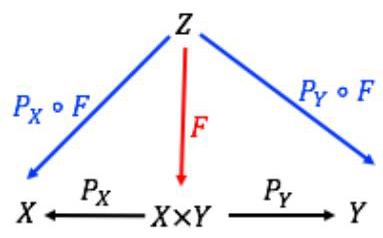
\includegraphics[max width=0.3\textwidth]{images/bo_d2bcsrref24c73avs720_42_640_1003_383_238_0.jpg}
\end{center}
\hspace*{3em} 

Figure 3.3: Diagram summarizing the statement (*)

namely,

the mapping \(F : Z \rightarrow  X \times  Y\) is continuous iff both \({P}_{X} \circ  F : Z \rightarrow  X\) and

\({P}_{Y} \circ  F : Z \rightarrow  Y\) are continuous. (*)

Proof. 1. For any open \(U\) , we imply \({p}_{X}^{-1}\left( U\right)  = U \times  Y \in  {\mathcal{B}}_{X \times  Y} \subseteq  {\mathcal{T}}_{X \times  Y}\) , i.e., \({p}_{X}^{-1}\left( U\right)\) is open. The same goes for \({p}_{Y}\) .

2. It suffices to show any topology \(\mathcal{T}\) that meets the condition in (2) must contain \({\mathcal{T}}_{\text{ product }}\) . We imply that for \(\forall U \in  {\mathcal{T}}_{X},V \in  {\mathcal{T}}_{Y}\) ,

\[
\left\{  {\begin{array}{l} {p}_{X}^{-1}\left( U\right)  = U \times  X \in  \mathcal{T} \\  {p}_{Y}^{-1}\left( V\right)  = X \times  V \in  \mathcal{T} \end{array} \Rightarrow  \left( {U \times  Y}\right)  \cap  \left( {X \times  V}\right)  = \left( {U \cap  X}\right)  \times  \left( {Y \cap  V}\right)  = U \times  V \in  \mathcal{T},}\right.
\]

which implies \({\mathcal{B}}_{X \times  Y} \subseteq  \mathcal{T}\) . Since \(\mathcal{T}\) is closed for union operation on subsets, we

imply \({\mathcal{T}}_{\text{ product topology }} \subseteq  \mathcal{T}\) .

3. (a) Firstly show that \({\mathcal{T}}_{\text{ product }}\) satisfies (*).

\begin{itemize}
\item For the forward direction, by (1) we imply both \({p}_{X} \circ  F\) and \({p}_{Y} \circ  F\) are continuous, since the composition of continuous functions are continuous as well.
\end{itemize}

\begin{itemize}
\item For the reverse direction, for \(\forall U \times  {\mathcal{T}}_{X},V \in  {\mathcal{T}}_{Y}\) ,
\end{itemize}

\[
{F}^{-1}\left( {U \times  V}\right)  = {\left( {p}_{X} \circ  F\right) }^{-1}\left( X\right)  \cap  {\left( {p}_{Y} \circ  F\right) }^{-1}\left( Y\right) ,
\]

which is open due to the continuity of \({p}_{X} \circ  F\) and \({p}_{Y} \circ  F\) .

(b) Then we show the uniqueness of \({\mathcal{T}}_{\text{ product }}\) . Let \(\mathcal{T}\) be another topology \(X \times  Y\) satisfying (*).

\begin{itemize}
\item Take \(Z = \left( {X \times  Y,\mathcal{T}}\right)\) , and consider the identity mapping \(F = \mathrm{{id}} : Z \rightarrow  Z\) , which is continuous. Therefore \({p}_{X} \circ  \mathrm{{id}}\) and \({p}_{Y} \circ  \mathrm{{id}}\) are continuous, i.e., \({p}_{X}\) and \({p}_{Y}\) are continuous. By (2) we imply \({\mathcal{T}}_{\text{ product }} \subseteq  \mathcal{T}\) .
\end{itemize}

\begin{itemize}
\item Take \(Z = \left( {X \times  Y,{\mathcal{T}}_{\text{ product }}}\right)\) , and consider the identity mapping \(F = \mathrm{{id}}\) : \(Z \rightarrow  Z\) . Note that \({p}_{X} \circ  F = {p}_{X}\) and \({p}_{Y} \circ  F = {p}_{Y}\) , which is continuous by (1). Therefore, the identity mapping \(F : \left( {X \times  Y,{\mathcal{T}}_{\text{ product }}}\right)  \rightarrow  \left( {X \times  Y,\mathcal{T}}\right)\) is continuous, which implies
\end{itemize}

\[
U = {\operatorname{id}}^{-1}\left( U\right)  \subseteq  {\mathcal{T}}_{\text{ product }}\text{ for }\forall U \in  \mathcal{T}\text{ , }
\]

i.e., \(\mathcal{T} \subseteq  {\mathcal{T}}_{\text{ product }}\) .

The proof is complete.

Definition 3.6 [Disjoint Union] Let \(X \times  Y\) be two topological spaces, then the disjoint union of \(X\) and \(Y\) is

\[
X\coprod Y \mathrel{\text{ := }} \left( {X\times \{ 0\} }\right)  \cup  \left( {Y\times \{ 1\} }\right)
\]

1. We define that \(U\) is open in \(X \coprod  Y\) if

(a) \(U \cap  \left( {X\times \{ 0\} }\right)\) is open in \(X \times  \{ 0\}\) ; and

(b) \(U \cap  \left( {Y\times \{ 1\} }\right)\) is open in \(Y \times  \{ 1\}\) .

We also need to show the well-definedness for this definition.

2. \(S\) is open in \(X \coprod  Y\) iff \(S\) can be expressed as

\[
S = \left( {U\times \{ 0\} }\right)  \cup  \left( {V\times \{ 1\} }\right)
\]

where \(U \subseteq  X\) is open and \(V \subseteq  Y\) is open.
\chapter{Properties of Topological Spaces}

\section*{3.6.2.1. Hausdorff Property}

Definition 3.7 [First Separation Axiom] A topological space \(X\) satisfies the first separation axiom if for any two distinct points \(x \neq  y \in  X\) , there exists open \(U \ni  x\) but not including \(y\) .

Proposition 3.11 A topological space \(X\) has first separation property if and only if for \(\forall x \in  X,\{ x\}\) is closed in \(X\) .

Proof. Sufficiency. Suppose that \(x \neq  y\) , then construct \(U \mathrel{\text{ := }} X \smallsetminus  \{ y\}\) , which is a open set that contains \(x\) but not includes \(y\) .

Necessity. Take any \(x \in  X\) , then for \(\forall y \neq  x\) , there exists \(y \in  {U}_{y}\) that is open and \(x \notin  {U}_{y}\) . Thus

\[
\{ y\}  \subseteq  {U}_{y} \subseteq  X \smallsetminus  \{ x\}
\]

which implies

\[
\mathop{\bigcup }\limits_{{y \in  X \smallsetminus  \{ x\} }}\{ y\}  \subseteq  \mathop{\bigcup }\limits_{{y \in  X \smallsetminus  \{ x\} }}{U}_{y} \subseteq  X \smallsetminus  \{ x\}
\]

i.e., \(X \smallsetminus  \{ x\}  = \mathop{\bigcup }\limits_{{y \in  X\smallsetminus \{ x\} }}{U}_{y}\) is open in \(X\) , i.e., \(\{ x\}\) is closed in \(X\) .

Definition 3.8 [Second separation Axiom] A topological space satisfies the second separation axiom (or \(X\) is Hausdorff) if for all \(x \neq  y\) in \(X\) , there exists open sets \(U,V\) such that

\[
x \in  U,\;y \in  V,\;U \cap  V = \varnothing
\]

\begin{itemize}
\item Example 3.13 All metrizable topological spaces are Hausdorff.
\end{itemize}

Suppose \(d\left( {x,y}\right)  = r > 0\) , then take \({B}_{r/2}\left( x\right)\) and \({B}_{r/2}\left( y\right)\)

\begin{itemize}
\item Example 3.14 Note that a topological space that is first separable may not necessarily be second separable:
\end{itemize}

Consider \({\mathcal{T}}_{\text{ co-finite }}\) , then \(X\) is first separable but not Hausdorff:

Suppose on the contrary that for given \(x \neq  y\) , there exists open sets \(U,V\) such that \(x \in  U,y \in  V\) , and

\[
U \cap  V = \varnothing  \Rightarrow  X = X \smallsetminus  \left( {U \cap  V}\right)  = \left( {X \smallsetminus  U}\right)  \cup  \left( {X \smallsetminus  V}\right) ,
\]

implying that the union of two finite sets equals \(X\) , which is infinite, which is a contradiction.

\section*{4.3. Monday for MAT4002}

There will be a quiz next Monday. The scope is everything before CNY holiday. There will be one question with four parts for 40 minutes.

\section*{4.3.1. Hausdorffness}

Reviewing. A topological space(X, T)is said to be Hausdorff (or satisfy the second separtion property), if given any distinct points \(x,y \in  X\) , there exist disjoint open sets \(U,V\) such that \(U \ni  x\) and \(V \ni  y\) .

Proposition 4.5 If the topological space(X, T)is Hausdorff, then all sequences \(\left\{  {x}_{n}\right\}\) in \(X\) has at most one limit.

Proof. Suppose on the contrary that

\[
\left\{  {x}_{n}\right\}   \rightarrow  a,\;\left\{  {x}_{n}\right\}   \rightarrow  b\text{ , with }a \neq  b
\]

By separation property, there exists \(U,V \in  \mathcal{T}\) and \(U \cap  V = \varnothing\) such that \(U \ni  a\) and \(V \ni  b\) .

By tie openness of \(U\) , there exists \(N\) such that \(\left\{  {{x}_{N},{x}_{N + 1},\ldots }\right\}   \subseteq  U\) , since \(\left\{  {x}_{n}\right\}   \rightarrow  a \in  U\) . Similarly, there exists \(M\) such that \(\left\{  {{x}_{M},{x}_{M + 1},\ldots }\right\}   \subseteq  V\) . Take \(K = \max \{ M,N\}  + 1\) , then \(\varnothing  \neq  U \cap  V \ni  {x}_{K}\) , which is a contradiction.

Proposition 4.6 Let \(X,Y\) be Hausdorff spaces. Then \(X \times  Y\) is Hausdorff with product topology.

Proof. Suppose that \(\left( {{x}_{1},{y}_{1}}\right)  \neq  \left( {{x}_{2},{y}_{2}}\right)\) in \(X \times  Y\) . Then \({x}_{1} \neq  {x}_{2}\) or \({y}_{1} \neq  {y}_{2}\) . w.l.o.g., assume that \({x}_{1} \neq  {x}_{2}\) , then there exists \(U,V\) open in \(X\) such that \({x}_{1} \in  U,{x}_{2} \in  V\) with \(U \cap  V = \varnothing\) .

Therefore, we imply \(\left( {U \times  Y}\right) ,\left( {V \times  Y}\right)  \in  {\mathcal{T}}_{X \times  Y}\) , and

\[
\left( {U \times  Y}\right)  \cap  \left( {V \times  Y}\right)  = \left( {U \cap  V}\right)  \cap  Y = \varnothing
\]

with \(\left( {{x}_{1},{y}_{1}}\right)  \in  U \times  Y,\left( {{x}_{2},{y}_{2}}\right)  \in  V \times  Y\) , i.e., \(X \times  Y\) is Hausdorff with product topology.

The same argument applies if the second separation property is replaced by first separation property.

Proposition 4.7 If \(f : X \rightarrow  Y\) is an injective continuous mapping, then \(Y\) is Hausdorff implies \(X\) is Hausdorff.

Proof. Suppose that \(Y\) satisfies the second separation property. For given \(a \neq  b\) in \(X\) , we imply \(f\left( a\right)  \neq  f\left( b\right)\) in \(Y\) . Therefore, there exists \(U \ni  f\left( a\right) ,V \ni  f\left( b\right)\) with \(U \cap  V = \varnothing\) . It follows that

\[
a \in  {f}^{-1}\left( U\right) ,b \in  {f}^{-1}\left( V\right) ,\;{f}^{-1}\left( U\right)  \cap  {f}^{-1}\left( V\right)  = {f}^{-1}\left( {U \cap  V}\right)  = \varnothing ,
\]

i.e., \(X\) is Hausdorff.

Corollary 4.1 If \(f : X \rightarrow  Y\) is homeomorphic, then \(X\) is Hausdorff iff \(Y\) is Hausdorff, i.e., Hausdorffness is a topological property (i.e., a property that is preserved under homeomorphism).

\section*{4.3.2. Connectedness}

Definition 4.4 [Connected] The topological space(X, T)is disconnected if there are open \(U,V \in  \mathcal{T}\) such that

\[
U \neq  \varnothing ,V \neq  \varnothing ,\;U \cap  V = \varnothing ,\;U \cup  V = X. \tag{4.4}
\]

If no such \(U,V \in  \mathcal{T}\) exist, then \(X\) is connected.

Proposition 4.8 Let(X, T)be topological spaces. TFAE (i.e., the followings are equivalent):

1. \(X\) is connected

2. The only subset of \(X\) which are both open and closed are \(\varnothing\) and \(X\)

3. Any continuous function \(f : X \rightarrow  \{ 0,1\}\) ( \(\{ 0,1\}\) is equipped with discrete topology) is a constant function.

Proof. (1) implies (2): Suppose that \(U \subseteq  X\) is both open and closed. Then \(U,X \smallsetminus  U\) are both open and disjoint, and \(U \cup  \left( {X \smallsetminus  U}\right)  = X\) . By connnectedness, either \(U = \varnothing\) or \(X \smallsetminus  U = \varnothing\) . Therefore, \(U = \varnothing\) or \(X\) .

(2) implies (3): Note that \(U = {f}^{-1}\left( {\{ 0\} }\right)\) and \(V = {f}^{-1}\left( {\{ 1\} }\right)\) are open disjoint sets in \(X\) satisfying \(U \cup  V = X\) . By the connectedness of \(X\) , either \(\left( {U,V}\right)  = \left( {X,\varnothing }\right)\) or \(\left( {V,U}\right)  = \left( {\varnothing ,X}\right)\) . In either case, we imply \(f\) is a constant function.

(3) implies (2): Suppose that \(U \subseteq  X\) is both open and closed. Construct the mapping

\[
f\left( x\right)  = \left\{  \begin{array}{ll} 0, & x \in  U \\  1, & x \in  X \smallsetminus  U \end{array}\right.
\]

It’s clear that \(f\) is continuous, and therefore \(f\left( x\right)  = 0\) or 1 . Therefore \(U = \varnothing\) or \(X\) .

(2) implies (1): Suppose on the contrary that there exists open \(U,V\) such that (4.4) holds. By (4.4), we imply \(U = X \smallsetminus  V\) is closed as well. Since \(U \neq  \varnothing\) and \(U = \varnothing\) or \(X\) , we imply \(U = X\) , which implies \(V = \varnothing\) , which is a contradiction.

\section*{Corollary 4.2 The interval \(\left\lbrack  {a,b}\right\rbrack   \subseteq  \mathbb{R}\) is connnected}

Proof. Suppose on the contrary that there exists continuous function \(f : \left\lbrack  {a,b}\right\rbrack   \rightarrow  \{ 0,1\}\) that takes 2 values. Construct the mapping \(\widetilde{f} : \left\lbrack  {a,b}\right\rbrack   \rightarrow  \mathbb{R}\)

\[
\widetilde{f} : \left\lbrack  {a,b}\right\rbrack  \overset{f}{ \rightarrow  }\{ 0,1\} \overset{i}{ \rightarrow  }\mathbb{R}
\]

\[
\text{ with }\widetilde{f} = i \circ  f\text{ . }
\]

Note that \(\{ 0,1\}  \subseteq  \mathbb{R}\) denotes the subspace topology, we imply the inclusion mapping \(i : \{ 0,1\}  \rightarrow  \mathbb{R}\) with \(s \mapsto  s\) is continuous. The composition of continuous mappings is continuous as well, i.e., \(\widetilde{f}\) is continuous.

Since the function \(f\) can take two values, there exists \(p,q \in  \left\lbrack  {a,b}\right\rbrack\) such that \(\widetilde{f}\left( p\right)  =\)  \(i \circ  f\left( p\right)  = 0\) and \(\widetilde{f}\left( q\right)  = i \circ  f\left( q\right)  = 1\) . By intermediate value theorem, there exists \(r \in  \left\lbrack  {a,b}\right\rbrack\) such that \(\widetilde{f}\left( r\right)  = i \circ  f\left( r\right)  = 1/2\) , which implies \(f\left( r\right)  = \frac{1}{2}\) , which is a contradiction.

Definition 4.5 [Connected subset] A non-empty subset \(S \subseteq  X\) is connected if \(S\) with the subspace topology is connected

Equivalently, \(S \subseteq  X\) is connected if, whenever \(U,V\) are open in \(X\) such that \(S \subseteq  U \cup  V\) , and \(\left( {U \cap  V}\right)  \cap  S = \varnothing\) , one can imply either \(U \cap  S = \varnothing\) or \(V \cap  S = \varnothing\) .

Proposition 4.9 If \(f : X \rightarrow  Y\) is continuous mapping, and the subset \(A \subseteq  X\) is connected, then \(f\left( A\right)\) is connected. In other words, the continuous image of a connected set is connected.

Proof. Suppose that \(U,V \subseteq  Y\) is open such that

\[
f\left( A\right)  \subseteq  U \cup  V,\;\left( {U \cap  V}\right)  \cap  f\left( A\right)  = \varnothing .
\]

Therefore we imply

\[
A \subseteq  {f}^{-1}\left( U\right)  \cup  {f}^{-1}\left( V\right) ,\;\left( {{f}^{-1}\left( U\right)  \cap  A}\right)  \cap  \left( {{f}^{-1}\left( V\right)  \cap  A}\right)  = \varnothing
\]

By connectedness of \(A\) , either \({f}^{-1}\left( U\right)  \cap  A = \varnothing\) or \({f}^{-1}\left( V\right)  \cap  A = \varnothing\) . Therefore, \(f\left( A\right)  \cap  U = \varnothing\) or \(f\left( A\right)  \cap  V = \varnothing\) , i.e., \(f\left( A\right)\) is connected.

Proposition 4.10 If \({\left\{  {A}_{i}\right\}  }_{i \in  I}\) are connnected and \({A}_{i} \cap  {A}_{j} \neq  \varnothing\) for \(\forall i,j \in  I\) , then the set \(\mathop{\bigcup }\limits_{{i \in  I}}{A}_{i}\) is connected.

Proof. Suppose the function \(f : { \cup  }_{i \in  I}{A}_{i} \rightarrow  \{ 0,1\}\) is a continuous map. Then we imply that its restriction \({\left. f\right| }_{{A}_{i}} = f \circ  i : {A}_{i} \rightarrow  \{ 0,1\}\) is continuous for all \(i \in  I\) . Thus \({\left. f\right| }_{{A}_{i}}\) is a constant for all \(i \in  I\) . Due to the non-empty intersection of \({A}_{i},{A}_{j}\) for \(\forall i,j \in  I\) , we imply \(f\) is constant.

Proposition 4.11 If \(X,Y\) are connnected, then \(X \times  Y\) is connected using product topology.

Proof. It’s clear that \(X \times  \left\{  {y}_{0}\right\}\) is connected in \(X \times  Y\) for fixed \({y}_{0}\) ; and \(\left\{  {x}_{0}\right\}   \times  Y\) is connected for fixed \({x}_{0}\) .

Therefore, for fixed \({y}_{0} \in  Y\) , construct \(B = X \times  \left\{  {y}_{0}\right\}\) and \({C}_{x} = \{ x\}  \times  Y\) , which follows that

\[
B \cap  {C}_{x} = \left\{  \left( {x,{y}_{0}}\right) \right\}   \neq  \varnothing ,\forall x \in  X \Rightarrow  B \cup  \left\{  {\mathop{\bigcup }\limits_{{x \in  X}}{C}_{x}}\right\}   = X \times  Y\text{ is connected. }
\]

Definition 4.6 [Path Connectes] Let(X, T)be a topological space.

1. A path connecting 2 points \(x,y \in  X\) is a continuous function \(\tau  : \left\lbrack  {0,1}\right\rbrack   \rightarrow  X\) with \(\tau \left( 0\right)  = x,\tau \left( 1\right)  = y\) .

2. \(X\) is path-connected if any 2 points in \(X\) can be connected by a path.

3. The set \(A \subseteq  X\) is path-connected, if \(A\) sastisfies the condition using subspace topology.

Or equivalently, \(A\) is path-connected if for any 2 points in \(X\) , there exists a continuous \(t : \left\lbrack  {0,1}\right\rbrack   \rightarrow  X\) with \(t\left( x\right)  \in  A\) for any \(x\) , connecting the 2 points.

\section*{4.6. Wednesday for MAT4002}

There will be a quiz on Monday.

Reviewing.

\begin{itemize}
\item Connectedness / Path-Connectedness
\end{itemize}

\section*{4.6.1. Remark on Connectedness}

Proposition 4.14 All path connected spaces \(X\) are connected.

Proof. Fix any \(x \in  X\) , for all \(y \in  X\) , there exists a continuous mapping \({p}_{y} : \left\lbrack  {0,1}\right\rbrack   \rightarrow  X\) such that

\[
{p}_{y}\left( 0\right)  = x,\;{p}_{y}\left( 1\right)  = y.
\]

Consider \({C}_{y} = {p}_{y}\left( \left\lbrack  {0,1}\right\rbrack  \right)\) , which is connected, due to proposition (4.9).

Note that \({\left\{  {C}_{y}\right\}  }_{y \in  X}\) is a collection of connected sets, and for any \(y,{y}^{\prime } \in  X,{C}_{y} \cap  {C}_{{y}^{\prime }} \ni\)  \(\{ x\}\) is non-empty. Applying proposition (4.10), we imply \(X = { \cup  }_{y \in  X}{C}_{y}\) is connected.

\begin{itemize}
\item Example 4.5 1. Exercise: if \(A \subset  B \subset  \bar{A}\) , then \(A\) is connected implies \(B\) is connected. (Hint: \(U \cap  A = \varnothing\) implies \(U \cap  \bar{A} = \varnothing\) for all open sets \(U\) in \(X\) .)
\end{itemize}

Proof. Suppose \(B\) is not connected, i.e., for any open \(U,V\) such that \(B \subseteq  U \cup  V\) and \(\left( {U \cap  V}\right)  \cap  B = \varnothing\) , we imply \(U \cap  B \neq  \varnothing\) and \(V \cap  B \neq  \varnothing\) , and therefore

\[
U \cap  \bar{A} \neq  \varnothing ,\;V \cap  \bar{A} \neq  \varnothing
\]

which implies

\[
U \cap  A \neq  \varnothing ,\;V \cap  A \neq  \varnothing
\]

which contradicts to the connectedness of \(A\) .

2. The converse of proposition (4.14) may not be necessarily true. Consider the so-called Topologist's comb example:

\begin{center}
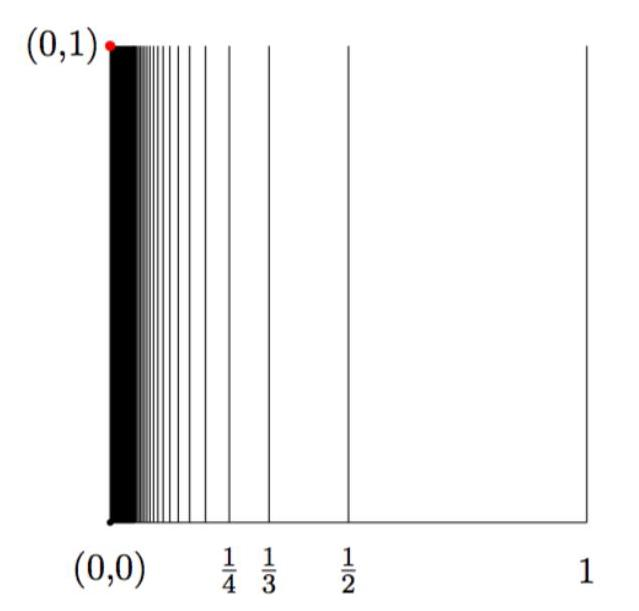
\includegraphics[max width=0.5\textwidth]{images/bo_d2bcsrref24c73avs720_52_671_318_639_611_0.jpg}
\end{center}
\hspace*{3em} 

Figure 4.1: Connected space \(X\) but not path-connected

Here we construct a connected space \(X \subseteq  {\mathbb{R}}^{2}\) but not path-connected shown in Fig (4.1), i.e., the union of the interval \(\left\lbrack  {0,1}\right\rbrack\) together with vertical line segments from \(\left( {1/n,0}\right)\) to \(\left( {1/n,1}\right)\) and the single point(0,1).

\[
X = \left( {\left\lbrack  {0,1}\right\rbrack  \times \{ 0\} }\right)  \cup  \mathop{\bigcup }\limits_{{n \geq  1}}\left( {\{ 1/n\}  \times  \left\lbrack  {0,1}\right\rbrack  }\right)  \cup  \left( {0,1}\right) .
\]

(a) Firstly, \(X\) is not path-connected. We show that there is no path in \(X\) links(0,1) to any other point, i.e., for continuous mapping \(p : \left\lbrack  {0,1}\right\rbrack   \rightarrow  X\) with \(p\left( 0\right)  = \left( {0,1}\right)\) , we may imply \(p\left( t\right)  = \left( {0,1}\right)\) for any \(t\) .

Define

\[
A = \{ t \in  \left\lbrack  {0,1}\right\rbrack   \mid  p\left( t\right)  = \left( {0,1}\right) \} .
\]

We claim that \(A = \left\lbrack  {0,1}\right\rbrack\) , i.e., suffices to show \(A\) is both open and closed in \(\left\lbrack  {0,1}\right\rbrack   :\)

i. The set \(A = {p}^{-1}\left( \left( {0,1}\right) \right)\) is nonempty and closed, since the pre-image of a closed set is closed as well.

ii. The set \(A\) is open: choose \({t}_{0} \in  A\) . By continuity of \(p\) , there exists \(\delta  > 0\) such that

\[
\parallel p\left( t\right)  - \left( {0,1}\right) \parallel  = \begin{Vmatrix}{p\left( t\right)  - p\left( {t}_{0}\right) }\end{Vmatrix} < \frac{1}{2},\;t \in  \left\lbrack  {0,1}\right\rbrack   \cap  \left( {{t}_{0} - \delta ,{t}_{0} + \delta }\right) .
\]

Since there is no point on the \(x\) -axis with the distance \(1/2\) to the point (0,1), we imply \(p\left( t\right)\) is not on the \(x\) -axis when \(t \in  \left\lbrack  {0,1}\right\rbrack   \cap  \left( {{t}_{0} - \delta ,{t}_{0} + \delta }\right)\) . Therefore, the \(x\) -coordinate of \(p\left( t\right)\) is either 0 or of the form \(1/n\) .

It suffices to show the open interval \(I \mathrel{\text{ := }} \left\lbrack  {0,1}\right\rbrack   \cap  \left( {{t}_{0} - \delta ,{t}_{0} + \delta }\right)\) is in \(A\) . Define the composite function \(f = x \circ  p : I \rightarrow  \mathbb{R}\) , where the mapping \(x : {\mathbb{R}}^{2} \rightarrow  \mathbb{R}\) is defined as \(\left( {a,b}\right)  \mapsto  a\) . Note that \(I\) is connected, we imply \(f\left( I\right)\) is connected, and \(f\left( I\right)\) belongs to \(\{ 0\}  \cup  \{ 1/n\}\) .

The only nonempty connected subset of \(\{ 0\}  \cup  \{ 1/n\}\) is a single point (left as exercise), and therefore \(f\left( I\right)\) is a single point. Since \(f\left( {t}_{0}\right)  = 0\) , we imply \(f\left( I\right)  = \{ 0\}\) , i.e., \(I \subseteq  A\) . Therefore \(A\) is open.

\section*{4.6.2. Compactness}

Compact set in \(X\) is used to generalize "closed and bounded" in \({\mathbb{R}}^{n}\) .

Definition 4.11 Let(X, T)be a topological space. A collection \(\mathcal{U} = \left\{  {{U}_{i} \mid  i \in  I}\right\}\) of open sets is an open cover of \(X\) if

\[
X = \mathop{\bigcup }\limits_{{i \in  I}}{U}_{i}
\]

A subcover of \(\mathcal{U}\) is a subfamily

\[
{\mathcal{U}}^{\prime } = \left\{  {{U}_{j} \mid  j \in  J}\right\}  ,\;J \subseteq  I
\]

such that \(\mathop{\bigcup }\limits_{{j \in  J}}{U}_{j} = X\) .

If \(J\) has finitely many elements, we say \({\mathcal{U}}^{\prime }\) is a finite subcover of \(X\) .

We say \(X\) is compact if any open cover of \(X\) has a finite subcover.

If \(A \subseteq  X\) has a subspace topology. then \(A\) is compact iff for any open collection of open sets (in \(X\) ) \(\left\{  {U}_{i}\right\}\) such that \(A \subseteq  \mathop{\bigcup }\limits_{{i \in  I}}{U}_{i}\) , there exists a fintie subcover \(A \subseteq  \mathop{\bigcup }\limits_{{k = 1}}^{n}{U}_{{i}_{k}}\) .

Proposition 4.15 Let \(X\) be a topological space. The followings are equivalent:

1. The space \(X\) is compact

2. If \(\left\{  {{V}_{i} \mid  i \in  I}\right\}\) is a collection of closed subsets in \(X\) such that

\[
\mathop{\bigcap }\limits_{{j \in  J}}{V}_{j} \neq  \varnothing ,\;\text{ for all finite }J \subseteq  I,
\]

then \({ \cap  }_{i \in  I}{V}_{i} \neq  \varnothing\) .

Compactness is an intrisical property, i.e., we do not need to worry about which underlying space for this definition.

\begin{itemize}
\item Example 4.6 1. \(X \subseteq  {\mathbb{R}}^{n}\) is compact iff \(X\) is closed and bounded. (Heine-Borel)
\end{itemize}

2. Let \(K \subseteq  {\mathbb{R}}^{n}\) be compact, then define the set

\(\mathcal{C}\left( K\right)  = \{\) all continuous mapping \(f : K \rightarrow  \mathbb{R}\}\)

Note that the \({d}_{\infty }\) metric associated with \(\mathcal{C}\left( K\right)\) , say \(\parallel f{\parallel }_{\infty } = \mathop{\sup }\limits_{{k \in  K}}f\left( k\right)\) , is well-defined.

Under the metric space \(\left( {\mathcal{C}\left( K\right) ,{d}_{\infty }}\right)\) , any \(\mathcal{J} \subseteq  \mathcal{C}\left( K\right)\) is compact, if and only if \(\mathcal{J}\) is

closed, bounded, and equi-continuous. (Aresul-Ascoli)

Therefore, we can see that the compactness is not equivalent to the closedness together with boundedness.

Proposition 4.16 Let \(X\) be a compact space, then all closed subset \(A \subseteq  X\) are compact.

Proof. Let \(\left\{  {{V}_{i} \mid  i \in  I}\right\}\) be a collection of closed subsets in \(A\) such that

\[
{ \cap  }_{j \in  J}{V}_{j} \neq  \varnothing ,\;\text{ for any finite }J \subseteq  I\text{ . }
\]

As \(A\) is closed in \(X\) , we imply \({V}_{j}\) is closed in \(X\) .

Due to the compactness of \(X\) and proposition (4.15), we imply

\[
{ \cap  }_{i \in  I}{V}_{i} \neq  \varnothing
\]

By the reverse direction of proposition (4.15), we imply \(A\) is compact.

Now consider the reverse direction of proposition (4.16), i.e., are all compact subsets \(K \subseteq  X\) closed in \(X\) ?

In general, the converse does not hold. Note that \(K = \{ x\}\) is compact for any topology \(X\) . However, there are some topologies such that \(\{ x\}\) is closed.

In order to obtain the converse of proposition (4.16), we need to obtain another

\section*{separation axiom:}

Proposition 4.17 Let \(X\) be Hausdorff, \(K \subseteq  X\) be compact, and \(x \in  X \smallsetminus  K\) . Then there exists open \(U,V \subseteq  X\) such that \(U \cap  V = \varnothing\) and

\[
U \cap  V = \varnothing ,\;K \subseteq  U,\;x \in  V.
\]

Proof. Let \(k \in  K\) , then by Hausdorffness, there exists open \({U}_{k} \ni  k,{V}_{k} \ni  x\) such that \({U}_{k} \cap  {V}_{k} = \varnothing\) . Therefore, \({\left\{  {U}_{k}\right\}  }_{k \in  K}\) forms an open cover of \(K\) . By compactness of \(K\) , \({\left\{  {U}_{{k}_{i}}\right\}  }_{i = 1}^{n}\) covers \(K\) . Constructing the set

\[
U \mathrel{\text{ := }} \mathop{\bigcup }\limits_{{i = 1}}^{n}{U}_{{k}_{i}},\;V = \mathop{\bigcap }\limits_{{i = 1}}^{n}{V}_{{k}_{i}}
\]

gives the desired result.

By making use of this separation axiom, we obtain the converse of proposition (4.16):

Corollary 4.3 All compact \(K\) in Hausdorff \(X\) is closed.

Proof. For \(\forall x \in  X \smallsetminus  K\) , by proposition (4.17) there exists open \(V\) such that \(x \in  V \subseteq  X \smallsetminus  K\) , and therefore \(X \smallsetminus  K\) is open.

\section*{5.3. Monday for MAT4002}

\section*{5.3.1. Continuous Functions on Compact Space}

Proposition 5.3 Let \(f : X \rightarrow  Y\) be continuous function on topological spaces, with \(A \subseteq  X\) compact. Then \(f\left( A\right)  \subseteq  Y\) is compact.

Proof. Let \(\left\{  {{U}_{i} \mid  i \in  I}\right\}\) be an open cover of \(f\left( A\right)\) , i.e.,

\[
f\left( A\right)  \subseteq  \mathop{\bigcup }\limits_{{i \in  I}}{U}_{i},\;{U}_{i} \in  {\mathcal{T}}_{Y}
\]

It follows that \(\left\{  {{f}^{-1}\left( {U}_{i}\right)  \mid  i \in  I}\right\}\) is an open cover of \(A\) :

\[
A \subseteq  {f}^{-1}\left( {\mathop{\bigcup }\limits_{{i \in  I}}{U}_{i}}\right)  = \mathop{\bigcup }\limits_{{i \in  I}}{f}^{-1}\left( {U}_{i}\right)
\]

By the compactness of \(A\) , there exists finite subcover of \(A\) :

\[
A \subseteq  \mathop{\bigcup }\limits_{{k = 1}}^{n}{f}^{-1}\left( {U}_{{i}_{k}}\right)
\]

which implies the constructed finite subcover of \(f\left( A\right)\) :

\[
f\left( A\right)  \subseteq  f\left( {{ \cup  }_{k = 1}^{n}{f}^{-1}\left( {U}_{{i}_{k}}\right) }\right)
\]

\[
= {\bigcup }_{k = 1}^{n}{U}_{{i}_{k}}
\]

lary 5.2 1. Suppose that \(X\) is compact, and the mapping \(f : X \rightarrow  \mathbb{R}\) is continuous, then \(f\left( X\right)\) is closed and bounded, i.e., there exists \(m,M \in  X\) such that

\[
f\left( m\right)  \leq  f\left( x\right)  \leq  f\left( M\right) ,\forall x \in  X.
\]

2. Suppose moreover that \(X\) is connected, then

\[
f\left( X\right)  = \left\lbrack  {f\left( m\right) ,f\left( M\right) }\right\rbrack  .
\]

Theorem 5.2 The space \(X,Y\) are compact iff \(X \times  Y\) is compact under product topology.

Proof. 1. Sufficiency: Given that \(X \times  Y\) is compact, consider the projection mapping (which is continuous):

\[
\left\{  \begin{array}{l} {P}_{X} : X \times  Y \rightarrow  X \\  {P}_{Y} : X \times  Y \rightarrow  Y \end{array}\right.
\]

By applying proposition (5.3), \({P}_{X}\left( {X \times  Y}\right)  = X,{P}_{Y}\left( {X \times  Y}\right)  = Y\) are both compact.

2. Necessity: Suppose that \({\left\{  {W}_{i}\right\}  }_{i \in  I}\) is an open cover of \(X \times  Y\) . Each open set \({W}_{i}\) can be written as:

\[
{W}_{i} = \mathop{\bigcup }\limits_{{j \in  {\mathcal{J}}_{i}}}{U}_{ij} \times  {V}_{ij},\;{U}_{ij} \in  {\mathcal{T}}_{X},{V}_{ij} \in  {\mathcal{T}}_{Y}.
\]

It follows that

\[
X \times  Y = \mathop{\bigcup }\limits_{{\left( {i,j}\right)  \in  K}}{U}_{ij} \times  {V}_{ij},\;K = \left\{  {\left( {i,j}\right)  \mid  i \in  I,j \in  {\mathcal{J}}_{i}}\right\}
\]

Therefore, it suffices to show \(\left\{  {{U}_{ij} \times  {V}_{ij} \mid  \left( {i,j}\right)  \in  K}\right\}\) has a finite subcover of \(X \times  Y\) .

\begin{itemize}
\item Note that \(X \times  \{ y\}  \subseteq  \mathop{\bigcup }\limits_{{\left( {i,j}\right)  \in  K}}{U}_{ij} \times  {V}_{ij}\) is compact for each \(y \in  Y\) , which implies there exists finite \({S}_{y} \in  K\) such that
\end{itemize}

\[
X \times  \{ y\}  \subseteq  \mathop{\bigcup }\limits_{{s \in  {S}_{y}}}{U}_{s} \times  {V}_{s}
\]

\begin{itemize}
\item w.l.o.g., assume that \(y \in  {V}_{s},\forall s \in  {S}_{y}\) , since we can remove the \({U}_{s} \times  {V}_{s}\) such that \(y \notin  {V}_{s}\) . Define the set \({V}_{y} \mathrel{\text{ := }} { \cap  }_{s \in  {S}_{y}}{V}_{s}\) , which is an open set containing \(y\) . We imply \({\left\{  {V}_{y}\right\}  }_{y \in  Y}\) forms an open cover of \(Y\) . By the compactness of \(Y\) ,
\end{itemize}

\[
\left\{  {{V}_{{y}_{1}},\ldots ,{V}_{{y}_{m}}}\right\}
\]

forms a finite subcover of \(Y\) .

\begin{itemize}
\item For each \(\ell  = 1,\ldots ,m\) ,
\end{itemize}

\[
X \times  \left\{  {y}_{\ell }\right\}   \subseteq  \mathop{\bigcup }\limits_{{s \in  {S}_{{y}_{\ell }}}}{U}_{s} \times  {V}_{s}
\]

Note that for any \(\left( {x,y}\right)  \in  X \times  Y\) , there exists \(\ell  \in  \{ 1,\ldots ,m\}\) such that \(y \in  {V}_{y\ell }\) ,

i.e., \(y \in  {V}_{s}\) for \(\forall s \in  {S}_{y\ell }\) . Therefore,

\[
X \times  Y = \mathop{\bigcup }\limits_{{\ell  = 1}}^{m}\mathop{\bigcup }\limits_{{s \in  {S}_{{y}_{\ell }}}}{U}_{s} \times  {V}_{s}
\]

Now pick

\[
{I}^{\prime } = \left\{  {i \in  I \mid  \left( {i,j}\right)  \in  { \cup  }_{\ell  = 1}^{m}{S}_{{y}_{\ell }}}\right\}  ,
\]

we imply \(X \times  Y = \mathop{\bigcup }\limits_{{{i}^{\prime } \in  {I}^{\prime }}}{W}_{i}\) and \({I}^{\prime }\) is finite.

Theorem 5.3 Suppose that \(X\) is compact, \(Y\) is Hausdorff, \(f : X \rightarrow  Y\) is continuous, bijective, then \(f\) is a homeomorphism.

Proof. It suffices to show \({f}^{-1}\) is continuous. Therefore, it suffices to show \({\left( {f}^{-1}\right) }^{-1}\left( V\right)\) is closed, given that \(V\) is closed in \(X\) :

Let \(V \subseteq  X\) be closed. Then \(V\) is compact, which implies \(f\left( V\right)\) is compact. Since \(f\left( V\right)  \subseteq  Y\) is Hausdorff, we imply \(f\left( V\right)\) is compact, i.e., \(f\left( V\right)\) is closed.

\section*{5.6. Wednesday for MAT4002}

\section*{5.6.1. Remarks on Compactness}

Theorem 5.5 \(X\) is compact, \(Y\) is Hausdorff, \(f : X \rightarrow  Y\) is continuous and bijective. Then \(X\) is homeomorphic to \(Y\)

Corollary 5.3 If \(X\) is compact, \(Y\) is Hausdorff, \(f : X \rightarrow  Y\) is injective and continous, then \(f : X \rightarrow  f\left( X\right)\) is homeomorphisc.

\begin{itemize}
\item Example 5.7 Here we give another proof for the fact that \({S}^{1} \times  {S}^{1}\) is homeomorphic to donut. Construct the mapping
\end{itemize}

\(f : \;{S}^{1} \times  {S}^{1} \rightarrow  {\mathbb{R}}^{3}\)

with \(\left( {{e}^{i\theta },{e}^{i\phi }}\right)  \mapsto  \left( {\left( {R + r\cos \theta }\right) \cos \phi ,\left( {R + r\cos \theta }\right) \sin \phi ,r\sin \theta }\right) \;\left( {R > r > 0}\right)\)

Note that:

\begin{itemize}
\item \(X = {S}^{1} \times  {S}^{1}\) is compact, \({\mathbb{R}}^{3}\) is Hausdorff;
\end{itemize}

\begin{itemize}
\item \(f\) is continuous and injective.
\end{itemize}

\begin{itemize}
\item \(f\left( {{S}^{1} \times  {S}^{1}}\right)\) is a "donut".
\end{itemize}

Therefore, we conclude that \({S}^{1} \times  {S}^{1}\) is homeomorphic to donut in \({\mathbb{R}}^{3}\) .

Definition 5.6 [Sequential Compactness] A topological space \(X\) is sequentially compact if every sequence in \(X\) has a convergent sub-sequence.

In \({\mathbb{R}}^{n}\) , the compactness is equivalent to sequential compactness. The same goes for any metric space(X, d). (Check notes for MAT3006)

However, compactness and sequential compactness is different for topological spaces in general.
\chapter{Quotient Space and Simplicial Complex}

In the end of Chapter 2, we introduced product space and disjoint union. In this Chapter, we give another way to construct new topological spaces from some old ones. This new way of construction is by gluing some special pieces from old topological spaces together.

The rough idea is as follows: Let \(X = \left\lbrack  {0,1}\right\rbrack   \times  \left\lbrack  {0,1}\right\rbrack\) (just like a piece of paper on a plane), we want to glue the leftmost edge with the rightmost edge to form a cylinder \({Y}_{1}\), as shown below:

\begin{center}
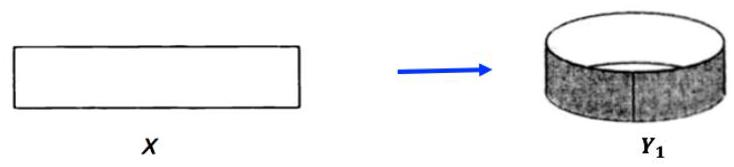
\includegraphics[width=0.5\textwidth]{images/Ch4_cylinder.jpg}
\end{center}
\hspace*{3em} 

If we give a half-twist to the strip before glue the ends together, we will get the Moebius strip \({Y}_{2}\) shown below:

\begin{center}
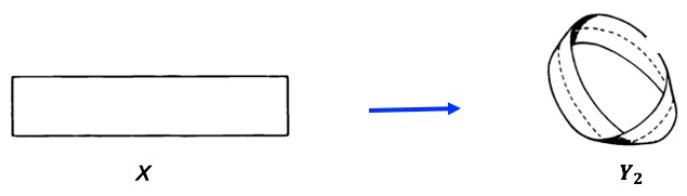
\includegraphics[width=0.5\textwidth]{images/Ch4_mobius1.jpg}
\end{center}
\hspace*{3em} 

Interestingly, the first topology \({Y}_{1}\) has two sides, while the second has only one side.

\section{Equivalence Relations and Equivalence Classes}

\begin{definition}[Equivalence Relation] \label{def:equiv_relation} The equivalence relation on a set \(X\) is a relation \~ such that

1. (Reflexive): \(x \sim  x,\forall x \in  X\)

2. (Symmetric): \(x \sim  y\) implies \(y \sim  x\)

3. (Transitive): \(x \sim  y\) and \(y \sim  z\) implies \(x \sim  z\).
\end{definition}

\begin{example} \label{eg:equiv_relation} 1. Let \(X = V\) be a vector space, and \(W \leq  V\) be a vector subspace. Define \({\mathbf{v}}_{1} \sim  {\mathbf{v}}_{2}\) if \({\mathbf{v}}_{1} - {\mathbf{v}}_{2} \in  W\).
(The well-definedness is left as exercise).

2. (Mobius Strip): Let \(X = \left\lbrack  {0,1}\right\rbrack   \times  \left\lbrack  {0,1}\right\rbrack\). We define \(\left( {{x}_{1},{y}_{1}}\right)  \sim  \left( {{x}_{2},{y}_{2}}\right)\) if

\begin{itemize}
\item \({x}_{1} = {x}_{2},{y}_{1} = {y}_{2}\) ; (e.g., \(\left( {{0.5},{0.6}}\right)  \sim  \left( {{0.5},{0.6}}\right)\) ) or
\end{itemize}

\begin{itemize}
\item \({x}_{1} = 0,{x}_{2} = 1\), and \({y}_{1} = 1 - {y}_{2}\) (e.g., \(\left( {0,1/4}\right)  \sim  \left( {1,3/4}\right)\) )
\end{itemize}

\begin{itemize}
\item \({x}_{1} = 1,{x}_{2} = 0\), and \({y}_{1} = 1 - {y}_{2}\) (e.g., \(\left( {1,3/4}\right)  \sim  \left( {0,1/4}\right)\) )
\end{itemize}
\end{example}

Another way to define an equivalence relation is to use partitions:
\begin{definition}[Partition] Let \(X\) be a nonempty set. A partition \(\mathcal{P} = \left\{  {{p}_{i} \mid  i \in  I}\right\}\) of \(X\) is a collection of subsets such that

1. \({P}_{i} \subseteq  X\) is non-empty

2. \({P}_{i} \cap  {P}_{j} = \varnothing\) if \(i \neq  j\)

3. \(\mathop{\bigcup }\limits_{{i \in  I}}{P}_{i} = X\).

Given a partition \(\mathcal{P} = \left\{  {{p}_{i} \mid  i \in  I}\right\}\), we can define an equivalence relation \(\sim\) on \(X\) by setting
\[
x \sim  y\;\text{ whenever }x,y \in  {p}_{i}\text{, for some }i \in  I
\]
\end{definition}
\begin{example}
Let \(X = \left\lbrack  {0,1}\right\rbrack   \times  \left\lbrack  {0,1}\right\rbrack\).
Then the partition 
\[
X = \{ \left( {x,y}\right) {\} }_{x \in  \left( {0,1}\right),y \in  \left\lbrack  {0,1}\right\rbrack  } \cup  \{ \left( {1,y}\right),\left( {0,1 - y}\right) {\} }_{y \in  \left\lbrack  {0,1}\right\rbrack  }
\]
gives the same equivalence relation as in part (2) in \autoref{eg:equiv_relation}.    
\end{example}

Conversely, for any equivalence relation \(\sim\) of $X$, we could form a corresponding partition of \(X\). This kind of partition is called the equivalence class:
\begin{definition}[Equivalence Class] Let \(X\) be a set with equivalence relation \(\sim\). The {\bf equivalence class} of an element \(x \in  X\) is
\[
\left\lbrack  x\right\rbrack   \mathrel{\text{:= }} \{ y \in  X \mid  x \sim  y\}.
\]
The collection of all equivalence classes is called the {\bf quotient space}:
\[
X/\sim\:= \{ \left\lbrack  x\right\rbrack   \mid  x \in  X\}.
\]
\end{definition}

\begin{example}
1. Consider the equivalence class defined in part (1) in \autoref{eg:equiv_relation}. The equivalence class has the form
\[
\left\lbrack  \mathbf{v}\right\rbrack   = \{ \mathbf{u} \in  V \mid  \mathbf{v} - \mathbf{u} \in  W\}  \mathrel{\text{:= }} \mathbf{v} + W.
\]
Therefore, the equivalence class is a generalization of the coset in linear algebra. Similarly, we define the set of generalized cosets as quotient space.
The quotient space \(V/ \sim\) reduces to the \(V/W\) in linear algebra:
\[
V/ \sim\   = \{ \left\lbrack  \mathbf{v}\right\rbrack   \mid  \mathbf{v} \in  V\}  = \{ \mathbf{v} + W \mid  \mathbf{v} \in  V\}  = V/W.
\]

2. Consider part (2) in \autoref{eg:equiv_relation} again. Then \(X/ \sim\) essentially forms the Mobius band. For instance, two `points' $\left\lbrack  \left( {1/2,1/2}\right) \right\rbrack, \left\lbrack  \left( {1,3/4}\right) \right\rbrack \in X/ \sim$ are:
\begin{align*}
\left\lbrack  \left( {1/2,1/2}\right) \right\rbrack   &= \{ \left( {1/2,1/2}\right) \} \\
\left\lbrack  \left( {1,3/4}\right) \right\rbrack   &= \{ \left( {1,3/4}\right),\left( {0,1/4}\right) \} = \left\lbrack  \left( {0,1/4}\right) \right\rbrack.
\end{align*}
Therefore, we have `glued' the two points $\left( {1,3/4}\right),\left( {0,1/4}\right)$ together into a single point in $X/\sim$.

3. Consider \(X = \left\lbrack  {0,1}\right\rbrack   \sqcup  \left\lbrack  {0,1}\right\rbrack\), i.e.,
\[
X = \left( {\left\lbrack  {0,1}\right\rbrack  \times \{ 0\} }\right)  \cup  \left( {\left\lbrack  {0,1}\right\rbrack  \times \{ 1\} }\right)
\] 
Take a partition on \(X\) by
\[
\{ \left( {a,0}\right) {\} }_{0 \leq  a < 1} \cup  \{ \left( {b,1}\right) {\} }_{0 < b \leq  1} \cup  \{ \left( {1,0}\right),\left( {0,1}\right) \}
\]
In other words, we `glue' the right end $(1,0)$ of the first segment to the left end $(0,1)$ of the second segment. As a result, the corresponding quotient space is plotted below:
\begin{center}
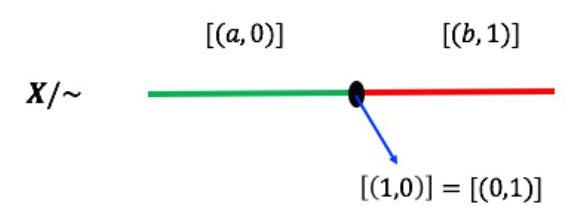
\includegraphics[width=0.4\textwidth]{images/Ch4_two_lines.jpg}
\end{center}

4. Let \(X = \left\lbrack  {0,1}\right\rbrack   \times  \left\lbrack  {0,1}\right\rbrack\). Consider the equivalence class with partition
\[
\{ \left( {a,b}\right) {\} }_{0 < a < 1;0 < b < 1} \cup  \{ \left( {x,0}\right),\left( {x,1}\right) {\} }_{0 \leq  x \leq  1} \cup  \{ \left( {0,y}\right),\left( {1,y}\right) {\} }_{0 < y < 1}
\]
The corresponding quotient space is plotted below:
\begin{center}
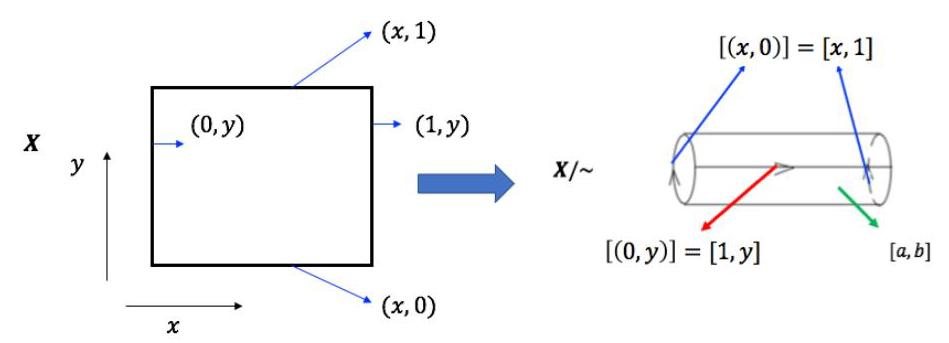
\includegraphics[width=0.8\textwidth]{images/Ch4_cylinder_glue.jpg}
\end{center}
\end{example}

\section{Quotient Topology}

Now given a topologcal space \(X\) and an equivalence relation \(\sim\) on it, our goal is to construct a topology on the space \(X/ \sim\).

\begin{proposition}[Quotient Topology] \label{prop:quotient_topology} Suppose $(X, \mathcal{T})$ is a topological space, and \(\sim\) is an equivalence relation on \(X\). Define the canonical projection map:
\[
p: \;X \rightarrow  X/ \sim  \quad \text{ with } \quad x \mapsto \left\lbrack  x\right\rbrack   
\]
which assigns each point \(x \in  X\) into the equivalence class \(\left\lbrack  x\right\rbrack\). Define a family of subsets \(\widetilde{\mathcal{T}}\) on \(X/ \sim\) by:
\[
\widetilde{U} \subseteq  X/ \sim  \text{ is in }\widetilde{\mathcal{T}}\text{ if }{p}^{-1}\left( \widetilde{U}\right) \text{ is in }\mathcal{T}
\]
Then \(\widetilde{\mathcal{T}}\) is a topology for \(X/ \sim\).  

We say $(X/\sim\, \widetilde{\mathcal{T}})$ the {\bf quotient topology} of the quotient space, and \(X/ \sim\).
\end{proposition}

\begin{proof} 1. \({p}^{-1}\left( {X/ \sim  }\right)  = X \in  \mathcal{T}\) and \({p}^{-1}\left( \varnothing \right)  = \varnothing  \in  \mathcal{T}\), which implies \(X/ \sim   \in  \widetilde{\mathcal{T}}\) and \(\varnothing  \in  \widetilde{\mathcal{T}}\).

2. Suppose that \(\widetilde{U},\widetilde{V} \in  \widetilde{\mathcal{T}}\), then we imply
\[
{p}^{-1}\left( \widetilde{U}\right),{p}^{-1}\left( \widetilde{V}\right)  \in  \mathcal{T} \Rightarrow  {p}^{-1}\left( {\widetilde{U} \cap  \widetilde{V}}\right)  \in  \mathcal{T},
\]
i.e., \(\widetilde{U} \cap  \widetilde{V} \in  \widetilde{\mathcal{T}}\).

3. Following the similar argument in (2), and the relation
\[
{p}^{-1}\left( {\bigcup {\widetilde{U}}_{i}}\right)  = \bigcup {p}^{-1}\left( {\widetilde{U}}_{i}\right),
\]
we conclude that \(\widetilde{T}\) is closed under countably union, and the proof is complete.
\end{proof}

\begin{remark}
1. \autoref{prop:quotient_topology} claims that \(\widetilde{U}\) is open in \(X/ \sim\) iff \({p}^{-1}\left( \widetilde{U}\right)\) is open in \(X\). The general question is that, does \(p\left( U\right)\) is open in \(X/ \sim\), given that \(U\) is open in \(X\) ? This may not necessarily hold. (See example (6.4)) In general \({p}^{-1}\left( {p\left( U\right) }\right)\) is strictly larger than \(U\), and may not be necessarily open in \(X\), even when \(U\) is open.

2. By definition, we can show that \(p\) is continuous.
\end{remark}

To fill the gap on the question shown in the remark, we consider the notion of the open mapping:
\begin{definition}\label{def:open_mapping} [Open Mapping] A function \(f: X \rightarrow  Y\) between two topological spaces is an open mapping if for each open \(U\) in \(X,f\left( U\right)\) is open in \(Y\).
\end{definition}


\begin{example} The mapping \(p: \left\lbrack  {0,1}\right\rbrack   \times  \left\lbrack  {0,1}\right\rbrack   \rightarrow  \left( {\left\lbrack  {0,1}\right\rbrack   \times  \left\lbrack  {0,1}\right\rbrack  }\right) / \sim\) sending the square to the Mobius band \(M\) is not an open mapping: Consider the open ball \(U = {B}_{1/2}\left( \left( {0,0}\right) \right)\) in \(\left\lbrack  {0,1}\right\rbrack   \times  \left\lbrack  {0,1}\right\rbrack\). Note that \(p\left( U\right)\) is open in \(M\) iff \({p}^{-1}\left( {p\left( U\right) }\right)\) is open in \(\left\lbrack  {0,1}\right\rbrack   \times  \left\lbrack  {0,1}\right\rbrack\). We can calculate \({p}^{-1}\left( {p\left( U\right) }\right)\) explicitly:
\[
{p}^{-1}\left( {p\left( U\right) }\right)  = U \cup  \{ \left( {1,y}\right)  \mid  1/2 \leq  y \leq  1\},
\]
which is not open.
\end{example}


\begin{proposition} A subset \(\widetilde{V}\) is closed in the quotient space \(X/ \sim\) iff \({p}^{1}\left( \widetilde{V}\right)\) is closed in \(X\), where \(p: X \rightarrow  X/ \sim\) denotes the canonical projection mapping.
\end{proposition}
\begin{proof} It follows from the fact that
\[
{p}^{-1}\left( {\left( {X/ \sim  }\right)  \smallsetminus  \widetilde{V}}\right)  = X \smallsetminus  {p}^{-1}\left( \widetilde{V}\right)
\]
\end{proof}
\begin{example} \label{eg:circle_glue} Consider \(X = \left\lbrack  {0,1}\right\rbrack\). We define \({x}_{1} \sim  {x}_{2}\) if:
\[
{x}_{1} = 0,{x}_{2} = 1\text{, or }{x}_{1} = 1,{x}_{2} = 0
\]
In other words, the partition on \(X\) is given by:
\[
X = \{ 0,1\}  \cup  \left( {\mathop{\bigcup }\limits_{{x \in  \left( {0,1}\right) }}\{ x\} }\right)
\]
The quotient space "glues" the endpoints of the interval \(\left\lbrack  {0,1}\right\rbrack\) together, shown in the figure below:
\begin{center}
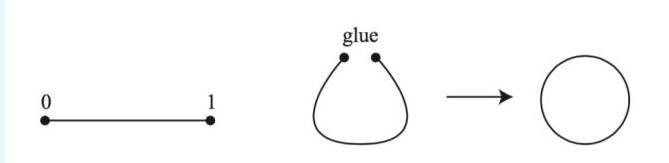
\includegraphics[width=0.6\textwidth]{images/Ch4_circle_glue.jpg}
\end{center}
It is intuitive that the constructed quotient space should be homeomorphic to a circle \({S}^{1}\). We will give a formal proof on this fact.
\end{example}

\begin{proposition} \label{prop:quotient_cont} Let \(X\) and \(Z\) be topological spaces, and \(\sim\) an equivalence relation on \(X\).
Let \(g: X/ \sim   \rightarrow  Z\) be a function, and \(p: X \rightarrow  X/ \sim\) is a projection mapping The mapping \(g\) is continuous if and only if \(g \circ  p: X \rightarrow  Z\) is continuous.
\end{proposition}

\begin{proof} 1. Necessity. Suppose that \(g\) is continuous. It’s clear that \(p\) is continuous, i.e, \(g \circ  p: X \rightarrow  Z\) is continuous.

2. Sufficiency. Suppose that \(g \circ  p: X \rightarrow  Z\) is continuous. Given any open \(U\) in \(Z\), we imply \({\left( g \circ  p\right) }^{-1}\left( U\right)  = {p}^{-1}{g}^{-1}\left( U\right)\) is open in \(X\). By definition of the quotient topology, we imply \({g}^{-1}\left( U\right)\) is open in \(X/ \sim\). Therefore, \(g\) is continuous.
\end{proof}

This useful lemma can be generalized into the case for generalized canonical projection mapping, called quotient mapping.

\begin{definition} \label{def:quotient_map}  A map \(p: X \rightarrow  Y\) between topological spaces is a quotient mapping if
\begin{enumerate}
    \item \(p\) is surjective; and
\item \(p\) is continuous;
\item For any \(U \subseteq  Y\) such that \({p}^{-1}\left( U\right)\) is open in \(X\), we imply \(U\) is open in \(Y\).
\end{enumerate}
\end{definition}

Obviously, the canonical projection map $p: X \to X/\sim$ is a quotient map. The advantage of quotient map is as given below:
\begin{proposition} \label{prop:quotient_cont2} Suppose that \(p: X \rightarrow  Y\) is a quotient map and that \(g: Y \rightarrow  Z\) is any mapping to another space \(Z\). Then \(g\) is continuous iff \(g \circ  p\) is continuous.
\end{proposition}
\begin{proof}
The proof follows similarly as in \autoref{prop:quotient_cont}.
\end{proof} 

Now we give a formal proof of the conclusion in \autoref{eg:circle_glue}:
\begin{proof} Define the mapping
\[
f: \;\left\lbrack  {0,1}\right\rbrack   \rightarrow  {S}^{1}
\quad 
\text{ with } \quad t \mapsto  \left( {\cos {2\pi t},\sin {2\pi t}}\right) \text{. }
\]
Since \(f\left( 0\right)  = f\left( 1\right)\), the function \(f\) induces a well-defined function
\[
g: \;\left\lbrack  {0,1}\right\rbrack  / \sim   \rightarrow  {S}^{1}
\quad
\text{ with }\quad \left\lbrack  t\right\rbrack   \mapsto  f\left( t\right)
\]
such that \(f = g \circ  p\), where \(p\) denotes the canonical projection mapping. Note that \(f\) is continuous. By \autoref{prop:quotient_cont2}, we imply \(g\) is continuous. Furthermore,
\begin{enumerate}
    \item Since \(\left\lbrack  {0,1}\right\rbrack\) is compact and \(p\) is continuous, we imply \(p\left( \left\lbrack  {0,1}\right\rbrack  \right)  = \left\lbrack  {0,1}\right\rbrack  / \sim\) is compact
\item \({S}^{1}\) is Hausdorff
\item \(g\) is a bijection
\end{enumerate}
By applying \autoref{thm:compact_hausdorff_homeo}, we conclude that \(g\) is a homeomorphism, i.e., \(\left\lbrack  {0,1}\right\rbrack  / \sim\) and \({S}^{1}\) are homeomorphic.
\end{proof}

The argument in the proof can be generalized into the proposition below:

\begin{proposition} \label{prop:quotient_homeo} Let \(f: X \rightarrow  Y\) be a surjective continuous mapping between topologcial spaces, and \(\sim\) be an equivalence relation on \(X\) defined by the partition \(\left\{  {{f}^{-1}\left( y\right)  \mid  y \in  Y}\right\}\) (i.e., \(x \sim  {x}^{\prime }\) iff \(f\left( x\right)  = f\left( {x}^{\prime }\right)\)). If \(X\) is compact and \(Y\) is Hausdorff, then \(X/ \sim\) and \(Y\) are homeomorphic.
\end{proposition}

The above proposition allows us to apply the following argument, which we shall use several times: To show 
\[X/ \sim\ \cong Y\] 
are homeomorphic, construct a surjective continuous mapping \(f: X \rightarrow  Y\) such that 
\begin{center}
\(f\left( {x}_{1}\right)  = f\left( {x}_{2}\right)\) whenever \({x}_{1} \sim  {x}_{2}\). 
\end{center}
Therefore, \(f\) will induce a well-defined function \(g: X/ \sim   \rightarrow  Y\) such that \(f = g \circ  p\). Then checking the conditions in \autoref{thm:compact_hausdorff_homeo} leads to the desired results.

\begin{example}
Consider \(X = \left\lbrack  {0,1}\right\rbrack   \times  \left\lbrack  {0,1}\right\rbrack\) and define \(\left( {{s}_{1},{t}_{1}}\right)  \sim  \left( {{s}_{2},{t}_{2}}\right)\) if one of the following holds:
\begin{itemize}
\item \({s}_{1} = {s}_{2}\) and \({t}_{1} = {t}_{2}\) ;
\item \(\left\{  {{s}_{1},{s}_{2}}\right\}   = \{ 0,1\},{t}_{1} = {t}_{2}\) ;
\item \(\left\{  {{t}_{1},{t}_{2}}\right\}   = \{ 0,1\}\) and \({s}_{1} = {s}_{2}\) ;
\item \(\left\{  {{s}_{1},{s}_{2}}\right\}   = \{ 0,1\},\left\{  {{t}_{1},{t}_{2}}\right\}   = \{ 0,1\}\)
\end{itemize}
We now show the corresponding quotient space \(\left( {\left\lbrack  {0,1}\right\rbrack   \times  \left\lbrack  {0,1}\right\rbrack  }\right) / \sim\) is hoemomorhpic to the torus \({\mathbb{T}}^{2}\): Define the mapping 
\[f: \left\lbrack  {0,1}\right\rbrack   \times  \left\lbrack  {0,1}\right\rbrack   \rightarrow  {\mathbb{T}}^{2} \quad \quad \left( {{t}_{1},{t}_{2}}\right)  \mapsto  \left( {{e}^{{2\pi i}{t}_{1}},{e}^{{2\pi i}{t}_{2}}}\right).\]
Then
\begin{itemize}
    \item \(f\) is surjective, which also implies \({\mathbb{T}}^{2} = f\left( {\left\lbrack  {0,1}\right\rbrack   \times  \left\lbrack  {0,1}\right\rbrack  }\right)\) is compact.

 \item \({\mathbb{T}}^{2}\) is Hausdorff.

\item It’s clear that \(\left( {{s}_{1},{t}_{1}}\right)  \sim  \left( {{s}_{2},{t}_{2}}\right)\) implies \(f\left( {{s}_{1},{t}_{1}}\right)  = f\left( {{s}_{2},{t}_{2}}\right)\). Conversely, suppose
\[
{e}^{{2\pi i}{s}_{1}} = {e}^{{2\pi i}{s}_{2}},\;{e}^{{2\pi i}{t}_{1}} = {e}^{{2\pi i}{t}_{2}}
\]
By the familiar property of \({e}^{ix}\), we imply either \({t}_{1} = {t}_{2}\) or \(\left\{  {{t}_{1},{t}_{2}}\right\}   = \{ 0,1\}\); and either \({s}_{1} = {s}_{2}\) or \(\left\{  {{s}_{1},{s}_{2}}\right\}   = \{ 0,1\}\)
\end{itemize}
By applying \autoref{prop:quotient_homeo}, we conclude that \(\left( {\left\lbrack  {0,1}\right\rbrack   \times  \left\lbrack  {0,1}\right\rbrack  }\right) / \sim\) is homeomorphic to \({\mathbb{T}}^{2}\).
\end{example}

\begin{example}
Consider the closed disk \({\mathbb{D}}^{2} = \left\{  {\left( {x,y}\right)  \in  {\mathbb{R}}^{2} \mid  {x}^{2} + {y}^{2} \leq  1}\right\}\), and define \(\left( {{x}_{1},{y}_{1}}\right)  \sim  \left( {{x}_{2},{y}_{2}}\right)\) by:
\begin{itemize}
\item \({x}_{1} = {x}_{2}\) and \({y}_{1} = {y}_{2}\) ;
\item \(\left( {{x}_{1},{y}_{1}}\right)\) and \(\left( {{x}_{2},{y}_{2}}\right)\) are in the boundary circle \({\mathbb{S}}^{1}\)
\end{itemize}
Then the corresponding quotient space \({\mathbb{D}}^{2}/ \sim\) is hoemomorhpic to the 2-dimension sphere \({\mathbb{S}}^{2} = \left\{  {\left( {x,y,z}\right)  \mid  {x}^{2} + {y}^{2} + {z}^{2} = 1}\right\}\): Define the mapping
\[f: \;{\mathbb{D}}^{2} \rightarrow  {\mathbb{S}}^{2} \]
by 
\begin{align*} 
\left( {0,0}\right)  &\mapsto  \left( {0,0,1}\right)\\
\left( {x,y}\right)  &\mapsto  \left( {\frac{x}{\sqrt{{x}^{2} + {y}^{2}}}\sin \left( {\pi \sqrt{{x}^{2} + {y}^{2}}}\right),\frac{y}{\sqrt{{x}^{2} + {y}^{2}}}\sin \left( {\pi \sqrt{{x}^{2} + {y}^{2}}}\right),\cos \left( {\pi \sqrt{{x}^{2} + {y}^{2}}}\right) }\right)
\end{align*}
It’s easy to check the conditions in \autoref{prop:quotient_homeo}, and we conclude that \({\mathbb{D}}^{2}/ \sim\)
is hoemomorhpic to \({\mathbb{S}}^{2}\).
\end{example}

In \autoref{prop:quotient_homeo}, we show the homeomorphism between \(X/ \sim\) and \(Y\) given the compactness of \(X\) and Hausdorffness of \(Y\). Now we show the generalize the proposition by replacing these conditions with the quotient mapping \(q\):
\begin{proposition} Suppose \(q: X \rightarrow  Y\) is a quotient map, and that \(\sim\) is an equivalence relation on \(X\) given by the partition \(\left\{  {{q}^{-1}\left( y\right)  \mid  y \in  Y}\right\}\). Then \(X/ \sim\) and \(Y\) are homeomorphic.
\end{proposition}
\begin{proof} Construct the mapping
\[
h: \;X/ \sim   \rightarrow  Y  \quad 
\text{ with } \quad h\left( \left\lbrack  x\right\rbrack  \right)  = q\left( x\right)
\]
Note that the mapping \(h\) is well-defined and bijective. And the quotient mapping \(q \mathrel{\text{:= }} h \circ  p\) is continuous by definition. By applying \autoref{prop:quotient_cont}, \(h\) is continuous, and we are only left to show that $h^{-1}$ is continuous, i.e. 
for any open \(\widetilde{U} \subseteq  X/ \sim\), \(h\left( \widetilde{U}\right)\) is open in \(Y\).

To see so, note that
\[
{q}^{-1}\left( {h\left( \widetilde{U}\right) }\right)  = {p}^{-1}{h}^{-1}\left( {h\left( \widetilde{U}\right) }\right)  = {p}^{-1}\left( \widetilde{U}\right),
\]
which is open by the definition of quotient topology. Therefore, \(h\left( \widetilde{U}\right)\) is open by (2) in \autoref{def:quotient_map}.
\end{proof}

\begin{example} \(\mathbb{R}/\mathbb{Z}\) is homeomorphic to the unit circle \({S}^{1}\): Indeed, consider the mapping
\[
q: \mathbb{R} \rightarrow  {S}^{1}
\quad \quad
x \mapsto  {e}^{2\pi ix}
\]
It is clear that

1. \(q\) is a continuous open mapping (why?)

2. \(q\) is surjective

Therefore, \(\mathbb{R}/ \sim   \cong  {S}^{1}\), provided that \(x \sim  y\) iff \(q\left( x\right)  = q\left( y\right)\), i.e., \(x - y \in  \mathbb{Z}\). Therefore,
\[
\mathbb{R}/\mathbb{Z} \cong  {S}^{1}
\]
\end{example}

\section{Simplicial Complex}
The idea of simplicial complex is to build some new spaces from some "fundamental" objects. The combinatorialists often study topology by the combinatorics of these fundamental objects. First we define what are the "fundamental" objects:

\begin{definition}[ \(n\) -simplex] \label{def:n_simplex} The standard \(n\) -simplex is the set
\[
{\Delta }^{n} = \left\{  {\left( {{x}_{1},\ldots,{x}_{n + 1}}\right)  \in  {\mathbb{R}}^{n + 1} \mid  {x}_{i} \geq  0,\forall i\text{ and }\mathop{\Sigma }\limits_{{i = 1}}^{{n + 1}}{x}_{i} = 1}\right\}
\]
The $0$, $1$, $2$ and $3$ simplices can be visualized as follows:
\begin{center}
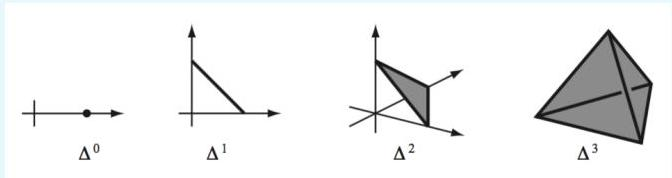
\includegraphics[width=0.7\textwidth]{images/Ch4_simplices.jpg}
\end{center}

1. The non-negative integer \(n\) is the \emph{dimension} of this simplex;

2. Its \emph{vertices}, denoted as \(V\left( {\Delta }^{n}\right)\), are those points \(\left( {{x}_{1},\ldots,{x}_{n + 1}}\right)\) in \({\Delta }^{n}\) such that \({x}_{i} = 1\) for some \(i\).

3. For each given non-empty \(\mathcal{A} \subseteq  \{ 1,\ldots,n + 1\}\), its \emph{facet} is defined as
\[
\left\{  {\left( {{x}_{1},\ldots,{x}_{n + 1}}\right)  \in  {\Delta }^{n} \mid  {x}_{i} = 0,\forall i \notin  \mathcal{A}}\right\}
\]
In particular, \({\Delta }^{n}\) is a face of itself

4. The \emph{inside} of \({\Delta }^{n}\) is
\[
\operatorname{inside}\left( {\Delta }^{n}\right)  \mathrel{\text{:= }} \left\{  {\left( {{x}_{1},\ldots,{x}_{n + 1}}\right)  \in  {\Delta }^{n} \mid  {x}_{i} > 0,\forall i}\right\}
\]
In particular, the inside of \({\Delta }^{0}\) is \({\Delta }^{0}\).
\end{definition}

\begin{definition}[Face Inclusion] A \emph{face inclusion} of \({\Delta }^{m}\) into \({\Delta }^{n}\left( {m < n}\right)\) is a function \({\Delta }^{m} \rightarrow  {\Delta }^{n}\) which comes from the restriction of an injective linear map \(f: {\mathbb{R}}^{m + 1} \rightarrow  {\mathbb{R}}^{n + 1}\) that maps vertices in \({\Delta }^{m}\) into vertices in \({\Delta }^{n}\).
\end{definition}

For example, the linear transformation \(f: {\mathbb{R}}^{2} \rightarrow  {\mathbb{R}}^{3}\) defined below is a face inclusion:
\[
f\left( {1,0}\right)  = \left( {0,1,0}\right),\;f\left( {0,1}\right)  = \left( {0,0,1}\right).
\]

\begin{remark} Any injection mapping from \(\{ 1,\ldots,m + 1\}  \rightarrow  \{ 1,\ldots,n + 1\}\) gives a face inclusion \({\Delta }^{m} \rightarrow  {\Delta }^{n}\), and vice versa.
\end{remark}

Now we build new spaces by gluing simplices together. This new space is called the simplicial complex. If a simplex is a part of the complex, so are all its faces.
\begin{definition}[Abstract Simplicial Complex] \label{def:simplicial_complex} An (abstract) simplicial complex is a pair \(K = \left( {V,\Sigma }\right)\), where \(V\) is a set of vertices and \(\Sigma\) is a collection of non-empty finite subsets of \(V\) (simplices) such that

1. For any \(v \in  V\), the 1-element set \(\{ v\}\) is in \(\Sigma\)

2. If \(\sigma\) is an element of \(\Sigma\), then so is any non-empty subset of \(\sigma\).
\end{definition}

For example, if \(V = \{ 1,2,3,4\}\), then one can take:
\begin{equation} \label{eq:sigma}
\Sigma  = \{ \{ 1\},\{ 2\},\{ 3\},\{ 4\},\{ 1,3,4\},\{ 2,4\},\{ 1,3\},\{ 3,4\},\{ 1,4\}. \}    
\end{equation}

We can associate to an abstract simplicial complex \(K\) a topological space \(\left| K\right|\), which is called its geometric realization:

\begin{definition}[Topological Realization] \label{def:topological_realization} The topological realization of \(K = \left( {V,\Sigma }\right)\) is a topological space \(\left| K\right|\) (or denoted as \(\left| \left( {V,\Sigma }\right) \right|\) ), where

1. For each \(\sigma  \in  \Sigma\) with \(\left| \sigma \right|  = n + 1\), take a copy of \(n\) -simplex and denote it as \({\Delta }_{\sigma }\)

2. Whenever \(\sigma  \subset  \tau  \in  \Sigma\), identify \({\Delta }_{\sigma }\) with a face of \({\Delta }_{\tau }\) through face inclusion.

Or equivalently, \(\left| K\right|\) is a quotient space of the disjoint union
\[
\mathop{\coprod }\limits_{{\sigma  \in  \Sigma }}\sigma
\]
by the equivalence relation which identifies a point \(y \in  \sigma\) with its image under the face inclusion \(\sigma  \rightarrow  \tau\), for any \(\sigma  \subset  \tau\).
\end{definition}

\begin{example} Take $(V,\Sigma)$ as in \autoref{eq:sigma}, so that
\begin{center}
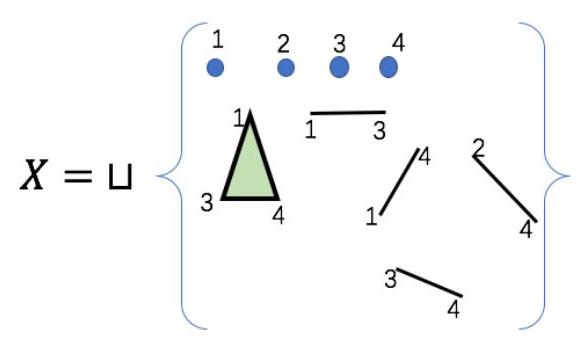
\includegraphics[width=0.6\textwidth]{images/Ch4_glue1.jpg}
\end{center}
Then its topological realization is:
\begin{center}
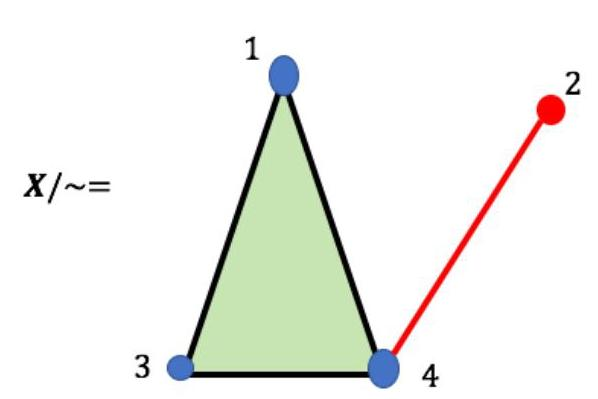
\includegraphics[width=0.4\textwidth]{images/Ch4_glue2.jpg}
\end{center}
\end{example} 

\begin{example} Take \(V = \{ 1,2,3,4\}\) and \(\Sigma  = \{\) all subsets of \(V\) except \(V\}\). 
Then its topological realization is \(\left| \left( {V,\Sigma }\right) \right|  = {\Delta }^{3}\) as shown in the figure below:
\begin{center}
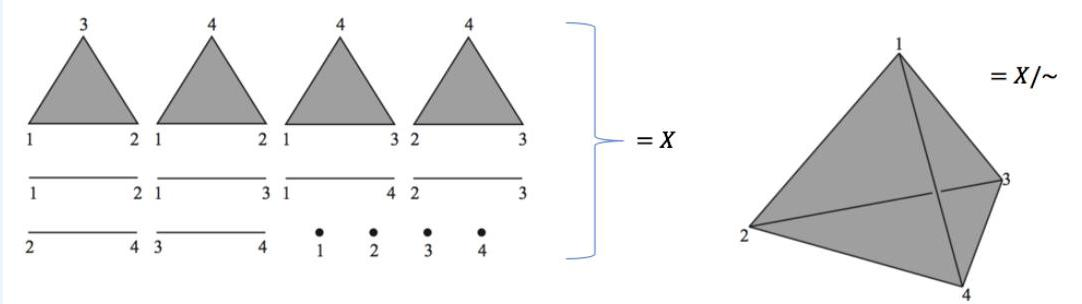
\includegraphics[width=0.9\textwidth]{images/Ch4_glue_3_simplex.jpg}
\end{center}
\end{example}

\begin{definition}[Triangulation] A \emph{triangulation} of a topological space \(X\) is a simplicial complex \(K = \left( {V,\Sigma }\right)\) together with a choice of homeomorphism \(\left| K\right|  \rightarrow  X\).
\end{definition}


\begin{example} \label{eg:tours_triangulation}
Consider the simplical complex \(K = \left( {V,\Sigma }\right)\) with
\[
V = \{ 1,2,3,4,\ldots,9\},\;\Sigma  = \left\{  \begin{array}{r} 9\text{ subsets with }1\text{ element } \\  {27}\text{ subsets with }2\text{ elements } \\  {18}\text{ subsets with }3\text{ elements } \end{array}\right.
\]
as given below. We start to build the topological realization of \(K\) with $9$ 0-simplicies, $27$ 1-simplicies, and $18$ 2-simplicies. The identification of them is as follows:
\begin{center}
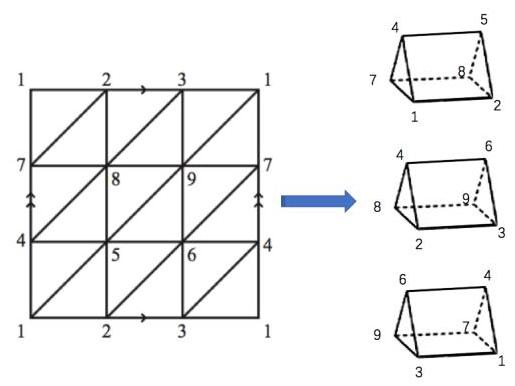
\includegraphics[width=0.6\textwidth]{images/Ch4_torus_triangle.jpg}
\end{center}
Step 1: Identify 3 columns separately, i.e., identify \(\{ 1,7,4,1,2,8,5,2\}\), \(\{ 2,8,5,2,3,9,6,3\}\), and \(\{ 3,9,6,3,1,7,4,1\}\).

\begin{center}
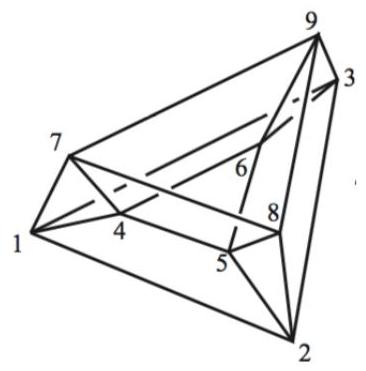
\includegraphics[width=0.3\textwidth]{images/Ch4_torus_triangle2.jpg}
\end{center}
Step 2: "glue" these three prisms in the figure above together. Then it will give us a `torus'. We will see in a moment that this $K = (V,\Sigma)$ is indeed a triangulation of $\mathbb{T}$.
\end{example}

\begin{example}
The simplicial complex below is a topological realization of \({S}^{2}\):
\begin{center}
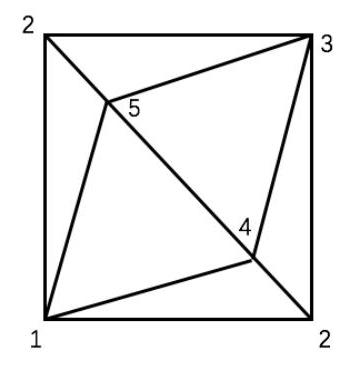
\includegraphics[width=0.4\textwidth]{images/Ch4_S1_triangle.jpg}
\end{center}
Indeed, $S^2$ is homeomorphic to the quotient space of $[0,1] \times [0,1]$ with the following identification:
\begin{center}
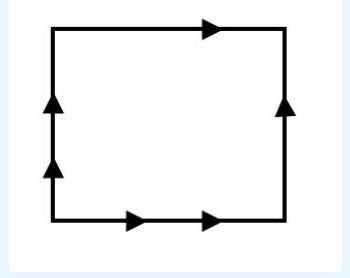
\includegraphics[width=0.5\textwidth]{images/Ch4_S1_quotient.jpg}
\end{center}
\end{example}

\begin{example}
One may ask whether one we build a triangulation of the tours using fewer simplices as in \autoref{eg:tours_triangulation}? The answer is no. 

For instance, one may think the number of triangles can be reduced as in the figure below: 
\begin{center}
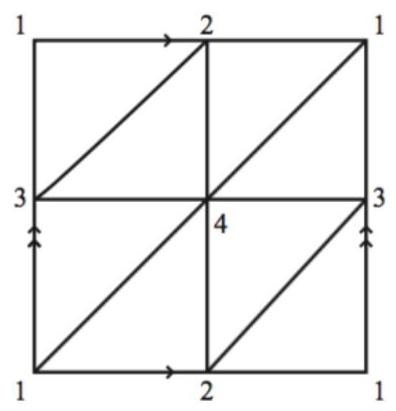
\includegraphics[width=0.4\textwidth]{images/Ch4_turous_nonex.jpg}
\end{center}
Howeverm if one pays attention to the bottom edge of the square, there are two 1-simplicies labelled \(\{ 1,2\}\), which means we have to 'glue the two bottom edges together, which cannot happen in the construction of torus.

As another example, the following diagram {\bf DOES NOT} give a triangulation of $S^2$:
\begin{center}
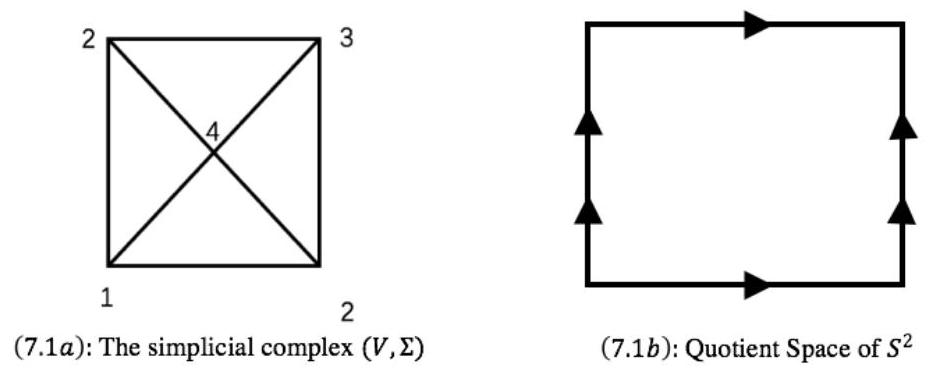
\includegraphics[width=0.6\textwidth]{images/Ch4_S2_nonex.jpg}
\end{center}
Note that the 2-simplex \({\Delta }_{\{ 2,3,4\} }\) appears twice in the left hand side of the figure. This means that we need to stick the top triangle and the right triangle together, which contradicts to the structure of the quotient space \({S}^{2}\) shown on the right hand side.
\end{example}

Simplicial complex gives us a combinatorial way to study \(X\), i.e. it suffices to study \(\left( {V,\Sigma }\right)\) such that \(\left| \left( {V,\Sigma }\right) \right|  \cong  X\). 
For example, if we want to distinguish \(\mathbb{T} = {S}^{1} \times  {S}^{1}\) and \({S}^{2}\), we just need  distinguish between their topological realizations. One way to do so is the following:

\begin{theorem}[Euler Characteristic] \label{thm:euler_char}
For any simplicial complex $(V,\Sigma)$, the Euler characteristic is defined by
\[\mathcal{X}(V,\Sigma) :=
\mathop{\sum }\limits_{{i = 1}}^{\infty }{\left( -1\right) }^{i}\text{ (number of subsets in }{\Sigma }\text{ with }\left( {i + 1}\right) \text{ -element) }
\]
Suppose that \(\left| \left( {{V}_{1},{\Sigma }_{1}}\right) \right|  \cong  \left| \left( {{V}_{2},{\Sigma }_{2}}\right) \right|\), then
\[\mathcal{X}\left( {{V}_{1},{\Sigma }_{1}}\right) = \mathcal{X}\left( {{V}_{2},{\Sigma }_{2}}\right).
\]
In particular, for two triangulations of the same topological space $X$, it has the same Euler characteristic. So we can define
$$\mathcal{X}(X) := \mathcal{X}(V,\Sigma)$$
for \emph{any} triangulation $|(V,\Sigma)| \cong X$ of $X$.
\end{theorem}

From previous examples, we can see that \(\mathcal{X}\left( {S}^{2}\right)  = 5 - 9 + 6 = 2\) and \(\mathcal{X}\left( \mathbb{T}\right)  = 9 - {27} + {18} = 0\), which implies
\[
{S}^{2} \ncong \mathbb{T}.
\]

\section{Properties of Simplicial Complex}
\begin{definition}[Simplicial Subcomplex] A subcomplex of a simplicial complex \(K = \left( {V,\Sigma }\right)\) is a simplicial complex \({K}^{\prime } = \left( {{V}^{\prime },{\Sigma }^{\prime }}\right)\) such that
\[
{V}^{\prime } \subseteq  V,\;{\Sigma }^{\prime } \subseteq  \Sigma
\]
\end{definition}

\begin{proposition} Suppose \({K}^{\prime }\) is subcomplex of \(K\), then \(\left| {K}^{\prime }\right|\) is closed in \(\left| K\right|\).
\end{proposition}
\begin{proof} Suppose that \(D\) is the disjoint union of all the simplicial complex forming \(\left| K\right|\) (note that the number of component in \(D\) is \(\left| \Sigma \right|\) )
Consider the canonical projection mapping 
\[p: D \rightarrow  \left| K\right|.\] Observe that \({p}^{-1}\left( \left| {K}^{\prime }\right| \right)\) precisely equals to \(\mathop{\coprod }\limits_{{{\sigma }^{\prime } \in  {\Sigma }^{\prime }}}{\sigma }^{\prime }\), which is closed in \(D\). By definition of quotient topology, \(\left| {K}^{\prime }\right|\) is also closed.
\end{proof}

\begin{definition} Let \(K = \left( {V,\Sigma }\right)\) be a simplicial complex and \({V}^{\prime } \subseteq  V\). Then the subcomplex spanned by \({V}^{\prime }\) is \(\left( {{V}^{\prime },{\Sigma }^{\prime }}\right)\) such that
\begin{itemize}
\item \({V}^{\prime }\) denotes the vertex set.
\item the simplices \({\Sigma }^{\prime }\) is given by
\[
\left\{  {\sigma  \in  \Sigma  \mid  \sigma  \subseteq  {V}^{\prime }}\right\}
\]
\end{itemize}
\end{definition}

\begin{definition} [Link and Star] \label{def:link_star} Let \(\left( {V,\Sigma }\right)  = K\) be a simplicial complex.
\begin{itemize}
\item The \emph{link} of \(v \in  V\), denoted as \(\operatorname{lk}\left( v\right)\) is the sub-complex with vertex set:
\[
\{ w \in  V \smallsetminus  \{ v\}  \mid  \{ v,w\}  \in  \Sigma \}
\]
and simplicies:
\[
\{ \sigma  \in  \Sigma  \mid  \mathbf{v} \notin  \sigma \text{ and }\sigma  \cup  \{ \mathbf{v}\}  \in  \Sigma \}
\]
\item The \emph{star} of \(v\) (denoted as \(\operatorname{st}\left( v\right)\) ) is
\[
\bigcup \{ \operatorname{inside}\left( \sigma \right)  \mid  \sigma  \in  \Sigma,v \in  \sigma \}
\]
\end{itemize}
\end{definition}

\begin{proposition} \(\mathrm{{st}}\left( v\right)\) is open and \(v \in  \mathrm{{st}}\left( v\right)\).
\end{proposition}
\begin{proof} Omitted - In fact, \(\left| K\right|  \smallsetminus  \operatorname{st}\left( v\right)\) is the simplicial subcomplex spanned by \(V\).
\end{proof}

\begin{proposition} Suppose that \(K = \left( {V,\Sigma }\right)\), where \(V\) is finite. Then \(\left| K\right|\) is compact.
\end{proposition}
\begin{proof} The mapping \(p: D \rightarrow  \left| K\right|\) is a canonical projection mapping, which is continuous; and \(D\) (the finite disjoint union of \({\Delta }_{\sigma }\) ’s) is compact.

Therefore, \(p\left( D\right)  = \left| K\right|\) is compact.
\end{proof}

\begin{proposition} For any simplicial complex \(K = \left( {V,\Sigma }\right)\), where \(V\) is finite, there is a continuous injection
\[
f: \left| K\right|  \rightarrow  {\mathbb{R}}^{n}\text{ for some }n
\]
\end{proposition}

\begin{proof} Let \(K^{\Pi} = \left( {V,\Sigma^{\Pi}}\right)\), where \(\Sigma^{\Pi} =\) power set of \(V\). Then
\[
\left| K^{\Pi}\right|  = {\Delta }^{\left| V\right|  - 1} \subseteq  {\mathbb{R}}^{\left| V\right| }
\]
Consider the inclusion
\[
i: \left| K\right|  \rightarrow  \left| K^{\Pi}\right|
\]
which comes from the following:

1. Consider the \(D \mathrel{\text{:= }} \mathop{\coprod }\limits_{{\sigma  \in  \Sigma }}{\Delta }_{\sigma }\) and \({D}^{\prime } = \mathop{\coprod }\limits_{{\Sigma^{\Pi} \in  \Sigma^{\Pi}}}{\Delta }_{\Sigma^{\Pi}}\) in \(\left( {V,\Sigma }\right)\) and \(\left( {V,\Sigma^{\Pi}}\right)\)

2. Construct the mapping \(\widetilde{i}: D \hookrightarrow  {D}^{\prime }\overset{{p}^{\prime }}{ \rightarrow  }\left| K\right|\).

3. The mapping \(\widetilde{i}\) descends to \(i: D/ \sim   \rightarrow  \left| K^{\Pi}\right|\) (try to write down the detailed mapping), which is continuous and injective.

Therefore, \(\left| K\right|  \hookrightarrow  \left| K^{\Pi}\right|  (\hookrightarrow  {\mathbb{R}}^{n})\), and the proof is complete.
\end{proof}

\begin{remark} 
More generally, if \(K = \left( V,\Sigma \right)\) is a simplicial subcomplex of \(\widetilde{K} = \left( {\widetilde{V},\widetilde{\Sigma}}\right)\), we can construct a continuous injection from \(\left| K\right|\) to \(\left| \widetilde{K}\right|\).

Let \({D}_{\Sigma } \mathrel{\text{:= }} \mathop{\coprod }\limits_{{\sigma  \in  \Sigma }}\sigma\) and \({D}_{\widetilde{\Sigma}} \mathrel{\text{:= }} \mathop{\coprod }\limits_{{\widetilde{\sigma} \in  \widetilde{\Sigma}}}\widetilde{\sigma}\), then \(\left| K\right|  = {D}_{\Sigma }/{ \sim  }_{\Sigma }\) and \(\left| \widetilde{K}\right|  = {D}_{\widetilde{\Sigma}}/{ \sim  }_{\widetilde{\Sigma}}\). It follows that
\[f:  {D}_{\Sigma } \rightarrow {D}_{\widetilde{\Sigma}} 
\overset{p}{ \rightarrow  }{D}_{\Sigma }/{ \sim  }_{\Sigma },\] 
where $p$ denotes the canonical projection mapping. Then \(f\) descends to a continuous mapping
\[
\widetilde{f}: {D}_{\Sigma }/{ \sim  }_{\Sigma } \rightarrow {D}_{\widetilde{\Sigma}}/{ \sim  }_{\widetilde{\Sigma}}
\]
Note that \(\widetilde{f}\) is injective since for all $x,y \in  {D}_{\Sigma }$:
\[
x{ \sim  }_{\widetilde{\Sigma}}y \quad \Leftrightarrow  \quad i\left( x\right) { \sim  }_{\widetilde{\Sigma}}\ i\left( y\right),
\]
where \(i: D_{\Sigma} \hookrightarrow D_{\widetilde{\Sigma}}\) denotes the inclusion mapping.
\end{remark}


\begin{proposition} If \(K = \left( {V,\Sigma }\right)\) with finite \(V\), then \(\left| K\right|\) is Hausdorff.
\end{proposition}

\begin{proof} Let \(g: \left| K\right| \hookrightarrow  {\mathbb{R}}^{n}\). Consider the bijective \(g: \left| K\right|  \rightarrow  g\left( \left| K\right| \right)\), which is continuous.
Since \(\left| K\right|\) is compact, and \(g\left( \left| K\right| \right)  \subseteq  {\mathbb{R}}^{n}\) is Hausdorff, we imply that \(\left| K\right|\) and \(g\left( \left| K\right| \right)\) are homeomorphic, i.e., \(\left| K\right|\) is Hausdorff.
\end{proof}

\begin{definition}[Edge Path] \label{def:edge_path} An edge path of \(K = \left( {V,\Sigma }\right)\) is a sequence of vertices \(\left( {{v}_{1},\ldots,{v}_{n}}\right),{v}_{i} \in  V\) such that \(\left\{  {{v}_{i},{v}_{i + 1}}\right\}   \in  \Sigma,\forall i\).
\end{definition}

\begin{proposition} Let \(K = \left( {V,\Sigma }\right)\) be a simplicial complex. TFAE:

1. \(\left| K\right|\) is connected

2. \(\left| K\right|\) is path-connected

3. Any 2 vertices in \(\left( {V,\Sigma }\right)\) can be joined by an edge path, i.e., for \(\forall u,v \in  V\), there exists \({v}_{1},\ldots,{v}_{k} \in  V\) such that \(\left( {u,{v}_{1},\ldots,{v}_{k},v}\right)\) is an edge path.
\end{proposition}

Sketch of Proof (to be revised). 1. (3) implies (2): For every \(x,y \in  \left| K\right|\),

\[
\left\{  \begin{array}{l} x \in  {\Delta }_{{\sigma }_{1}}\text{ for some }{\sigma }_{1} \in  \Sigma. \\  y \in  {\Delta }_{{\sigma }_{2}}\text{ for some }{\sigma }_{2} \in  \Sigma. \end{array}\right.
\]

Take a path joining \(x\) to a vertex \({v}_{1} \in  {\sigma }_{1}\) and a path joining \(y\) to a vertex \({v}_{2} \in  {\sigma }_{2}\). By (3), we have a path joining \({v}_{1}\) and \({v}_{2}\).

2. (1) implies (3): Suppose on the contrary that there is a vertex \(v\) not satisfying (3). Take \({V}^{\prime }\) as the set of vertexs that can be joined with \(v\) ; and \({V}^{\prime \prime }\) as the set of vertexs that cannot be joinied with \(v\).

Then \({V}^{\prime },{V}^{\prime \prime } \neq  \varnothing\). Consider \({K}^{\prime },{K}^{\prime \prime }\) be simplicial subcomplexes of \(K\), spanned by \({V}^{\prime }\) and \({V}^{\prime \prime }\). Then \(\left| {K}^{\prime }\right|,\left| {K}^{\prime \prime }\right|\) are disjoint, closed in \(\left| K\right|\).

\(\left| K\right|  = \left| {K}^{\prime }\right|  \cup  \left| {K}^{\prime \prime }\right|\). If there exists \(x \in  \left| K\right|  \smallsetminus  \left( {\left| {K}^{\prime }\right|  \cup  \left| {K}^{\prime \prime }\right| }\right)\), then for any \(\sigma  \in  \Sigma\) such that \(x \in  {\Delta }_{\sigma }\), we imply \({\Delta }_{\sigma } \nsubseteq  \left| {K}^{\prime }\right|\) or \(\left| {K}^{\prime \prime }\right|\).

Therefore, \(\sigma\) consists of vertices in both \({V}^{\prime }\) and \({V}^{\prime \prime }\). Then there is \({v}^{\prime },{v}^{\prime \prime } \in  \sigma\) joining \({V}^{\prime }\) and \({V}^{\prime \prime }\).

Therefore, there is no such \(x\) and hence \(\left| K\right|  = \left| {K}^{\prime }\right|  \cup  \left| {K}^{\prime \prime }\right|\) is a disjoint union of two closed sets, i.e., not connected.
\chapter{Homotopy}
To understand an object \(X\) (in our focus, \(X\) denotes topological space), one may try to understand functions
\[
f : A \rightarrow  X, \;\text{ or }\;g : X \rightarrow  B
\]
One special example is to let \(B = \mathbb{R}\). As for two topological spaces, there are many continuous mappings from \(X\) to \(Y\). We will group all these mappings into equivalence classes by checking whether $f$ can be `continuously deformed' to $g$.
\begin{definition} \label{def:homotopy} [Homotopy] A \emph{homotopy} between two continuous maps \(f, g : X \rightarrow  Y\) is a continuous map
\[
H : X \times  \left\lbrack  {0, 1}\right\rbrack   \rightarrow  Y
\]
such that
\[
H\left( {x, 0}\right)  = f\left( x\right), \;H\left( {x, 1}\right)  = g\left( x\right)
\]
If such \(H\) exists, we say \(f\) and \(g\) are homotopic, denoted as 
\[f \simeq  g.\]
\end{definition}
\begin{example} \label{eg:homotopy_convex} Let \(Y \subseteq  {\mathbb{R}}^{2}\) be a convex subset. Consider two continuous maps \(f : X \rightarrow  Y\) and \(g : X \rightarrow  Y\). They are always homotopic since we can define the homotopy
\[
H\left( {x, t}\right)  = {tg}\left( x\right)  + \left( {1 - t}\right) f\left( x\right).
\]
\end{example}

\begin{example} In the picture below, one can take 
\begin{center}
$X = [0,H] \times [0,W]$, $Y = [0,255] \times [0,255] \times [0,255]$ \quad and \quad
$f, g: X \to Y$
\end{center}
$f(h,w) := (r_0,g_0,b_0)$ and $g(h,w) := (r_1,g_1,b_1)$ are the pixels of the leftmost and rightmost picture at coordinate point $(h,w)$ respectively. 

The homotopy $H: X \times [0,1] \to Y$
is a continuous `deformation' of the pixels on the picture. For instance, the pixels of the pictures are continuously deformed by
$$H\left((h,w),0\right) = f(h,w) \ \ \to\ \  H\left((h,w),\frac{1}{3}\right)\ \ \to\ \  H\left((h,w),\frac{2}{3}\right) \ \ \to\ \ H\left((h,w),1\right) = g(h,w).$$
\begin{center}
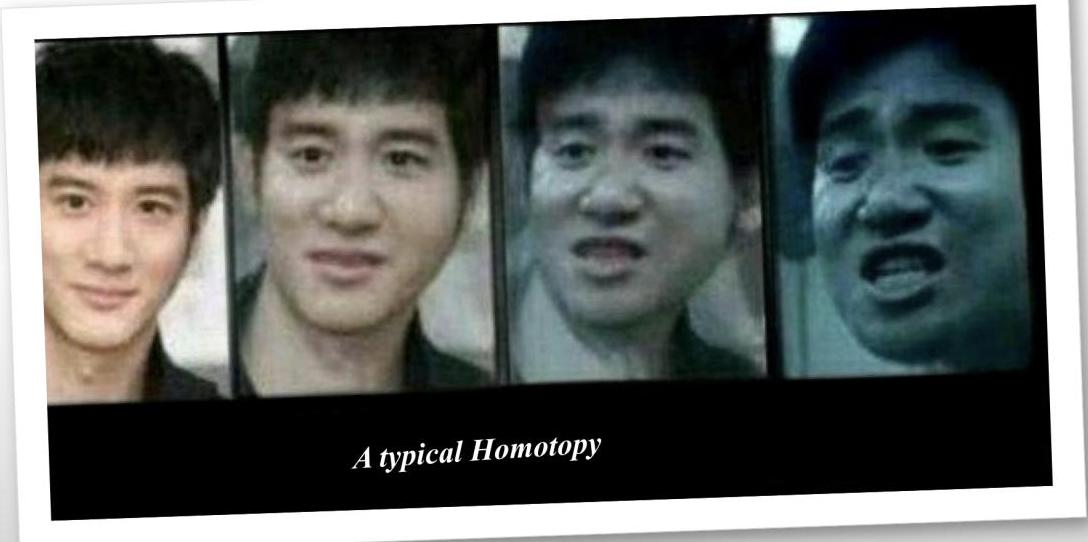
\includegraphics[width=0.8\textwidth]{images/Ch5_Cheung.jpg}
\end{center}
\end{example}

\begin{proposition} Homotopy is an equivalence relation.
\end{proposition}

\begin{proof} 1. Let \(f : X \rightarrow  Y\) be any continuous map. Then \(f \simeq  f\) : we can define a homotopy \(H\left( {x, t}\right)  = f\left( x\right), \forall 0 \leq  t \leq  1\).

2. Suppose \(f \simeq  g\), i.e., \(H\) is a homotopy between \(f\) and \(g\), then \(g \simeq  f\) : Define the mapping \({H}^{\prime }\left( {x, t}\right)  = H\left( {x, 1 - t}\right)\), then
\[
{H}^{\prime }\left( {x, 0}\right)  = g\left( x\right), \;{H}^{\prime }\left( {x, 1}\right)  = f\left( x\right)
\]

3. Let \(f, g, h : X \rightarrow  Y\) be three continuous maps. If \(f\) and \(g\) are homotopic and \(g\) and \(h\) are homotopic, then \(f\) and \(h\) are homotopic: Let \(H : X \times  \left\lbrack  {0, 1}\right\rbrack   \rightarrow  Y\) be a continuous map such that
\[
H\left( {x, 0}\right)  = f\left( x\right), H\left( {x, 1}\right)  = g\left( x\right) ;
\]
\(K : X \times  \left\lbrack  {0, 1}\right\rbrack   \rightarrow  Y\) be a continuous map such that
\[
K\left( {x, 0}\right)  = g\left( x\right), K\left( {x, 1}\right)  = h\left( x\right).
\]
Define a function \(J : X \times  \left\lbrack  {0, 1}\right\rbrack   \rightarrow  Y\) by
\[
J\left( {x, t}\right)  = \left\{  \begin{matrix} H\left( {x, {2t}}\right), & 0 \leq  t \leq  1/2 \\  K\left( {x, {2t} - 1}\right), & 1/2 \leq  t \leq  1 \end{matrix}\right.
\]
Then \(J\) is continuous, since for all closed \(V \subseteq  Y\), 
\[
{J}^{-1}\left( V\right)  = \left( {{J}^{-1}\left( V\right)  \cap  \left( {X \times  \left\lbrack  {0, 1/2}\right\rbrack  }\right) }\right)  \cup  \left( {{J}^{-1}\left( V\right)  \cap  \left( {X \times  \left\lbrack  {1/2, 1}\right\rbrack  }\right) }\right)  = {H}^{-1}\left( V\right)  \cup  {K}^{-1}\left( V\right), 
\]
and the closedness of \({H}^{-1}\left( V\right)\) and \({K}^{-1}\left( V\right)\) implies the closedness of \({J}^{-1}\left( V\right)\).

Moreover, \(J\) has the property that \(J\left( {x, 0}\right)  = H\left( {x, 0}\right)  = f\left( x\right)\), while \(J\left( {x, 1}\right)  =\)  \(K\left( {x, 1}\right)  = h\left( x\right)\).
\end{proof}


Back to \autoref{eg:homotopy_convex}: If \(Y \subseteq  {\mathbb{R}}^{n}\) is convex, then the set of continuous functions \(f : X \rightarrow  Y\) form a single equivalence class. In other words, all such maps are homotopic to each other.

\begin{proposition} \label{prop:comp_homotopy} Consider four continuous mappings
\[
W\overset{f}{ \rightarrow  }X, \;X\overset{g}{ \rightarrow  }Y, \;X\overset{h}{ \rightarrow  }Y, \;Y\overset{k}{ \rightarrow  }Z.
\]
If \(g \simeq  h\), then
\[
g \circ  f \simeq  h \circ  f, \;k \circ  g \simeq  k \circ  h
\]
\end{proposition}
\begin{proof} Suppose there exists the homotopy \(H : g \simeq  h\), then \(k \circ  H : X \times  I \rightarrow  Z\) gives the homotopy between \(k \circ  g\) and \(k \circ  h\).

Similarly, \(H \circ  \left( {f \times  {\operatorname{id}}_{I}}\right)  : W \times  I \rightarrow  Y\) gives the homotopy \(g \circ  f \simeq  h \circ  f\).
\end{proof}

\begin{definition} \label{def:homotopy_equivalence} [Homotopy Equivalence] Two topological spaces \(X\) and \(Y\) are homotopy equivalent if there are continuous maps \(f : X \rightarrow  Y\), and \(g : Y \rightarrow  X\) such that
\begin{align*}
g \circ  f &\simeq  {\operatorname{id}}_{X \rightarrow  X}
\\
f \circ  g &\simeq  {\operatorname{id}}_{Y \rightarrow  Y}, 
\end{align*}
which is denoted as \(X \simeq  Y\). 
\end{definition}

\begin{proposition}
Let $X$ and $Y$ be topological spaces.
\begin{enumerate}
    \item If \(X \cong  Y\) are homeomorphic, then they are homotopic equivalent.
    \item The homotopy equivalence \(X \simeq  Y\) gives a bijection between \(\{ \phi  :\) continuous \(W \rightarrow\)  \(X\} / \sim\) and \(\{ \phi\) : continuous \(W \rightarrow  Y\} / \sim\), for any given topological space \(W\).
    \item The homotopy equivalence \(X \simeq  Y\) forms an equivalence relation between topological spaces.
\end{enumerate}
\end{proposition}

\begin{proof} Since \(X \simeq  Y\), we can find \(f : X \rightarrow  Y\) and \(g : Y \rightarrow  X\) such that \(f \circ  g \simeq\)  \({\mathrm{{id}}}_{Y}\) and \(g \circ  f \simeq  {\mathrm{{id}}}_{X}\). We construct a mapping
\[\alpha  : \;\{ \phi  : W \rightarrow  X\ | \ \phi \text{ continuous}\} / \sim \ \longrightarrow  \{ \phi  : W \rightarrow  Y\ | \ \phi \text{ continuous}\} / \sim\]
by \(\left\lbrack  \phi \right\rbrack   \mapsto  \left\lbrack  {f \circ  \phi }\right\rbrack\). Then one can check \(\alpha\) is well-defined, since \({\phi }_{1} \sim  {\phi }_{2}\) implies \(f \circ  {\phi }_{1} \sim  f \circ  {\phi }_{2}\).

Also, we can construct a mapping
\[\beta  : \;\{ \phi  :W \rightarrow  Y\ | \ \phi \text{ continuous}\} / \sim \  \longrightarrow  \{ \phi  :W \rightarrow  X\ | \ \phi \text{ continuous}\} / \sim\]
by \(\left\lbrack  \psi \right\rbrack   \mapsto  \left\lbrack  {g \circ  \phi }\right\rbrack\). Similarly, \(\beta\) is well-defined.

Now one can check that \(\alpha  \circ  \beta  = \mathrm{{id}}\) and \(\beta  \circ  \alpha  = \mathrm{{id}}\). For example, 
\[
\alpha  \circ  \beta \left\lbrack  \psi \right\rbrack   = \left\lbrack  {f \circ  g \circ  \psi }\right\rbrack   = \left\lbrack  \psi \right\rbrack , 
\]
where the last equality is due to the fact that \(f \circ  g \simeq  {\operatorname{id}}_{Y}\).

3. is left as an exercise.
\end{proof}

Compared with homeomorphism, some properties are lost when we consider homotopy equivalence.
\begin{definition} \label{def:contractible} [Contractible] The topological space \(X\) is \emph{contractible} if it is homotopy equivalent to any point \(\{ \mathbf{c}\}\).

In other words, there exists continuous mappings \(f, g\) such that
\[
\{ \mathbf{c}\} \overset{f}{ \rightarrow  }X\overset{g}{ \rightarrow  }\{ \mathbf{c}\}, g \circ  f \simeq  {\operatorname{id}}_{\{ \mathbf{c}\} }
\]
\[
X\overset{g}{ \rightarrow  }\{ \mathbf{c}\} \overset{f}{ \rightarrow  }X, f \circ  g \simeq  {\operatorname{id}}_{X}
\]
\end{definition}

Note that \(g \circ  f \simeq  {\operatorname{id}}_{\{ c\} }\) follows naturally; and since \(X \cong  X\), we can find \(f, g\) such that \(f \circ  g = {c}_{y}\) for some \(y \in  X\), where \({c}_{y} : X \rightarrow  X\) is a constant function \({c}_{y}\left( x\right)  = y, \forall x \in  X\). Therefore, to check \(X\) is contractible, it suffices to check \({c}_{y} \simeq  {\operatorname{id}}_{X}, \forall y \in  X\) Therefore, \(X\) is contractible if its identity map \({\operatorname{id}}_{X}\) is homotopic to any constant map \({c}_{y}, \forall y \in  X\).

\begin{proposition} The definition for $X$ being contractible can be simplified further:

1. \(X\) is contractible if it is homotopy equivalent to some point \(\{ c\}\)

2. \(X\) is contractible if the identity map \({\operatorname{id}}_{X}\) is homotopic to some constant map
\[
{c}_{y}\left( x\right)  = y.
\]
\end{proposition}

\begin{proof} The only thing is to show that \({c}_{y} \simeq  {c}_{{y}^{\prime }}, \forall y, {y}^{\prime } \in  X\). By homework 3, \(X\) is path-connected, and therefore there exists continuous \(p\left( t\right)\) such that
\[
p\left( 0\right)  = y, \;p\left( 1\right)  = {y}^{\prime }
\]
Therefore, we construct the homotopy between \({c}_{y}\) and \({c}_{{y}^{\prime }}\) as follows:
\[
H\left( {x, t}\right)  = p\left( t\right).
\]
\end{proof}

\begin{example} \(X = {\mathbb{R}}^{2}\) is contractible:
It suffices to show that the mapping \(f\left( \mathbf{x}\right)  = \mathbf{x}, \forall \mathbf{x} \in  {\mathbb{R}}^{2}\) is homotopic to the constant function \(g\left( x\right)  = \left( {0, 0}\right), \forall x \in  {\mathbb{R}}^{2}\), i.e., \(g = {c}_{\left( 0, 0\right) }\).

Consider the continuous mapping \(H\left( {\mathbf{x}, t}\right)  = {tf}\left( \mathbf{x}\right)\), with
\[
H\left( {\mathbf{x}, 0}\right)  = {c}_{\left( 0, 0\right) }, \;H\left( {\mathbf{x}, 1}\right)  = {\operatorname{id}}_{X}
\]
Therefore, \({c}_{\left( 0, 0\right) } \simeq  {\mathrm{{id}}}_{X}\). Since \({c}_{\left( 0, 0\right) } \simeq  {c}_{\mathbf{y}}, \forall \mathbf{y} \in  {\mathbb{R}}^{2}\), we imply \({c}_{\mathbf{y}} \simeq  {\mathrm{{id}}}_{X}\) for any \(\mathbf{y} \in  {\mathbb{R}}^{2}\). Therefore, \(X\) is contractible. More generally, any convex \(X \subseteq  {\mathbb{R}}^{n}\) is contractible.
\end{example}

\begin{remark}
\({S}^{1}\) is not contractible, and we will see later. In particular, we are not able to construct the continuous mapping
\[
H : {S}^{1} \times  \left\lbrack  {0, 1}\right\rbrack   \rightarrow  {S}^{1}
\]
such that
\[
H\left( {{e}^{2\pi ix}, 0}\right)  = {e}^{2\pi ix}, \;H\left( {{e}^{2\pi ix}, 1}\right)  = {e}^{{2\pi i}\left( 0\right) } = 1
\]
One may ask - how about the mapping \(H\left( {{e}^{2\pi ix}, t}\right)  = {e}^{2\pi ixt}\)? Unfortunately, it is not well-defined, since
\[
H\left( {{e}^{{2\pi i}\left( 1\right) }, t}\right)  = {e}^{2\pi it} = H\left( {{e}^{{2\pi i}\left( 0\right) }, t}\right)  = 1
\]
and the equality is not true for \(t \neq  0, 1\).
\end{remark}

\begin{definition} \label{def:homotopy_retract} [Homotopy Retract] Let \(A \subseteq  X\) and \(i : A \hookrightarrow  X\) be an inclusion. We say \(A\) is a \emph{homotopy retract} of \(X\) if there exists continuous mapping \(r : X \rightarrow  A\) such that
\[
r \circ  i : A \hookrightarrow  X\overset{r}{ \rightarrow  }A = {\operatorname{id}}_{A}
\]
\[
i \circ  r : X\overset{r}{ \rightarrow  }A \hookrightarrow  X \simeq  {\operatorname{id}}_{X}
\]
In particular, \(A \simeq  X\).
\end{definition}
\begin{example} The $1$-sphere \({S}^{1}\) is a homotopy retract of Mobius band \(M\). More explicitly, 
let \(M = {\left\lbrack  0, 1\right\rbrack  }^{2}/ \sim\) and \({S}^{1} = \left\lbrack  {0, 1}\right\rbrack  / \sim\) by the appropriate equivalence relations. Then the inclusion \(i\) and the retraction \(r\) are given by:
\[i(\left\lbrack  x\right\rbrack)  :=  \left\lbrack  \left( {x, \frac{1}{2}}\right) \right\rbrack
\]
\[r\left\lbrack  \left( {x, y}\right) \right\rbrack  :=  \left\lbrack  x\right\rbrack
\]
As a result, 
\[
r \circ  i = {\operatorname{id}}_{{S}^{1}}, \;i \circ  r\left( \left\lbrack  \left( {x, y}\right) \right\rbrack  \right)  = \left\lbrack  \left( {x, 1/2}\right) \right\rbrack
\]
It suffices to show \(i \circ  r \simeq  {\mathrm{{id}}}_{M}\), where \({\mathrm{{id}}}_{M}\left( \left\lbrack  \left( {x, y}\right) \right\rbrack  \right)  = \left\lbrack  \left( {x, y}\right) \right\rbrack\).
To do so, construct the continuous mapping \(H : M \times  I \rightarrow  M\) with
\[
H\left( {\left\lbrack  \left( {x, y}\right) \right\rbrack , t}\right)  \mathrel{\text{ := }} \left\lbrack  \left( {x, \left( {1 - t}\right) y + t/2}\right) \right\rbrack
\]
To show the well-definedness of \(H\), we need to check
\[
H\left( {\left\lbrack  \left( {0, y}\right) \right\rbrack , t}\right)  = H\left( {\left\lbrack  \left( {1, 1 - y}\right) \right\rbrack , t}\right), \;\forall y \in  \left\lbrack  {0, 1}\right\rbrack
\]
It’s clear that \(H\) gives a homotopy between \(i \circ  r\) and \({\mathrm{{id}}}_{M}\), i.e., \(i \circ  r \simeq  {\mathrm{{id}}}_{M}\)
\end{example}

\begin{example} The \(n - 1\) -sphere \({S}^{n - 1}\) is a homotopy retract of \({\mathbb{R}}^{n} \smallsetminus  \{ \mathbf{0}\}\): Consider the usual inclusion \(i : {S}^{n - 1} \rightarrow  {\mathbb{R}}^{n} \smallsetminus  \{ 0\}\) and
\[
r : \;{\mathbb{R}}^{n} \smallsetminus  \{ 0\}  \rightarrow  {\mathbb{S}}^{n - 1}
\]
with $r(x) = \frac{x}{\parallel x\parallel }$. Therefore, \(r \circ  i = {\operatorname{id}}_{{S}^{n - 1}}\) and \(i \circ  r\left( x\right)  = \frac{x}{\parallel x\parallel }\).

It suffices to show that \(i \circ  r \simeq  {\operatorname{id}}_{{\mathbb{R}}^{n}\smallsetminus \{ 0\} }\). To see so, consider the homotopy 
\[H\left( {x, t}\right)  = {tx} + (1 -t)\mathbf{x}/\parallel \mathbf{x}\parallel.\] 
Then $H$ is well-defined, since \(H\left( {x, t}\right)  \in  {\mathbb{R}}^{n} \smallsetminus  \{ \mathbf{0}\}\) for all \(\mathbf{x} \in  {\mathbb{R}}^{n} \smallsetminus  \{ \mathbf{0}\}\) and \(t \in  \left\lbrack  {0, 1}\right\rbrack\).

Note that 
\[
H\left( {\mathbf{x}, 0}\right)  = i \circ  r\left( \mathbf{x}\right), \;H\left( {\mathbf{x}, 1}\right)  = \mathbf{x} = \operatorname{id}\left( \mathbf{x}\right)
\]
so the result follows.
\end{example}

\begin{definition} \label{def:relative_homotopy} [Homotopic Relative] Let \(A \subseteq  X\) be topological spaces. We say \(f, g : X \rightarrow  Y\) are homotopic relative to \(A\) if there exists \(H : X \times  I \rightarrow  Y\) such that
\[
\left\{  {\begin{array}{l} H\left( {x, 0}\right)  = f\left( x\right) \\  H\left( {x, 1}\right)  = g\left( x\right)  \end{array}\;\text{ and }H\left( {a, t}\right)  = f\left( a\right)  = g\left( a\right), \forall a \in  A}\right.
\]
\end{definition}

\section{Simplicial Approximation Theorem}
In this section, we wish to understand homotopy between simplicial complexes \(f, g : \left| K\right|  \rightarrow  \left| L\right|\)

\begin{definition} [Simplicial Map] A simplicial map between \({K}_{1} = \left( {{V}_{1}, {\sum }_{1}}\right)\) and \({K}_{2} =\)  \(\left( {{V}_{2}, {\sum }_{2}}\right)\) is a mapping \(f : {K}_{1} \rightarrow  {K}_{2}\) such that

1. It maps vertices to vertices

2. It maps simplicies to simplicies, i.e., 
\[
f\left( {\sigma }_{1}\right)  \in  {\sum }_{2}, \forall {\sigma }_{1} \in  {\sum }_{1}, 
\]
\end{definition}

\begin{example} Consider the simplicial complexes defined as follows:
\begin{center}
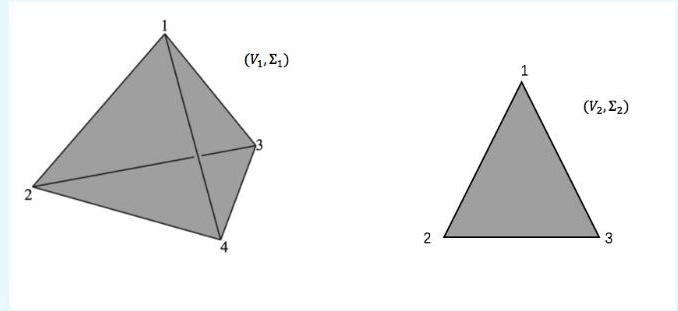
\includegraphics[width=0.5\textwidth]{images/Ch5_simplex_map.jpg}
\end{center}
In particular, \(\{ 1, 2, 3, 4\}  \notin  {\sum }_{1}\) and \(\{ 1, 2, 3\}  \in  {\sum }_{2}\). Then we can define the simplicial map as:
\[
f\left( 1\right)  = 1, \;f\left( 2\right)  = 2, \;f\left( 3\right)  = 3, \;f\left( 4\right)  = 3
\]
In particular, \(f\left( {\{ 1, 2, 4\} }\right)  = \{ 1, 2, 3\}  \in  {\sum }_{2}\).
\end{example}

Now we want to define the simplicial map between the topological realizations. There are several observations:
\begin{enumerate}
\item We have seen that each \(\left| K\right|  \subseteq  {\mathbb{R}}^{m}\) for some \(m\). In particular, \(m = \# V - 1\).

\item Each point \(x \in  \left| K\right|\) lies uniquely on an inside of some \({\Delta }_{\sigma }\), , where \(\sigma  \in  \sum\).

\item Suppose that the vertices of \({K}_{1}\) are \({V}_{1} = \left\{  {{u}_{1}, \ldots, {u}_{n}}\right\}   \subseteq  {\mathbb{R}}^{m}\). Then every \(\mathbf{x} \in  {K}_{1}\) can be uniquely written as
\[
\mathbf{x} = \mathop{\sum }\limits_{{i = 1}}^{k}{\alpha }_{i}{U}_{{\sigma }_{i}}
\]
with \({\alpha }_{i} > 0, \sum {\alpha }_{i} = 1\) and \(\sigma  = \left\{  {{U}_{{\sigma }_{1}}, \ldots, {U}_{{\sigma }_{k}}}\right\}\) is the unique simplex where \(x \in\) inside \(\left( {\Delta }_{\sigma }\right)\).
\begin{center}
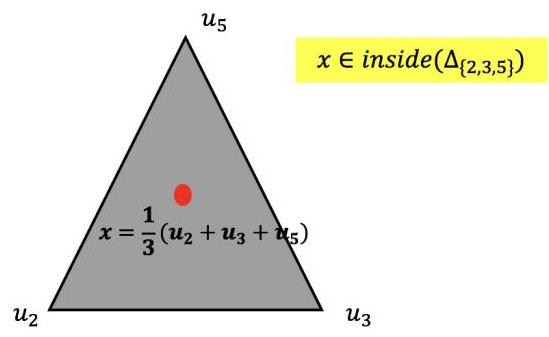
\includegraphics[width=0.4\textwidth]{images/Ch5_inside_coords.jpg}
\end{center}
\item Our simplicial map \(f\) maps \({V}_{1}\) to \({V}_{2} = \left\{  {{w}_{1}, \ldots, {w}_{p}}\right\}   \subseteq  {\mathbb{R}}^{m}\), so for each \(i\), we have \(f\left( {\mathbf{u}}_{i}\right)  = {\mathbf{w}}_{j}\) for some \(j \in  \{ 1, \ldots, p\}.\)
\end{enumerate}

\begin{definition} [Mapping induced from Simplicial Mapping] The simplicial map \(f : {K}_{1} \rightarrow\)  \({K}_{2}\) induces a mapping \(\left| f\right|  : \left| {K}_{1}\right|  \rightarrow  \left| {K}_{2}\right|\) between the topological realizations such that

\begin{enumerate}
    \item It maps vertexes to vertexes, i.e., \(\left| f\right| \left( {v}_{1}\right)  = f\left( {v}_{1}\right), \forall {v}_{1} \in  V\left( {K}_{1}\right)\).

\item it is affine, i.e., 
\[
\left| f\right| \left( {\mathop{\sum }\limits_{{i = 1}}^{k}{\alpha }_{i}{v}_{i}}\right)  = \mathop{\sum }\limits_{{i = 1}}^{k}{\alpha }_{i}\left| f\right| \left( {v}_{i}\right)
\]
\end{enumerate}
(note that \(\left| f\right|  : \left| {K}_{1}\right|  \rightarrow  \left| {K}_{2}\right|\) is continuous).
\end{definition}

Here is our more refined goal: Suppose we are given a continuous map \(\left| g\right|  : \left| K\right|  \rightarrow  \left| L\right|\), we want to approximate \(\left| g\right|\) by \(\left| f\right|\), where \(f : K \rightarrow  L\) is a simplicial map. It is obvious that \(f\) is an easier object to study compared with \(\left| g\right|\).

However, we cannot achieve this goal unless we subdivide \(K\) into smaller pieces:

\begin{definition} [Subdivision] Let \(K\) be a simplicial complex. A simplicial complex \({K}^{\prime }\) is called a \emph{subdivision} of \(K\) if

\begin{enumerate}
    \item Each simplex of \({K}^{\prime }\) is contained in a simplex of \(K\)

\item Each simplex of \(K\) equals the union of finitely many simplices of \({K}^{\prime }\)
\end{enumerate} 
As a result, we can form an homeomorphism \(h : \left| {K}^{\prime }\right|  \rightarrow  \left| K\right|\) such that for each \({\sigma }^{\prime } \in  {\sum }_{{K}^{\prime }}\), there exists \(\sigma  \in  {\sum }_{K}\) satisfying
\[
f\left( {\Delta }_{{\sigma }^{\prime }}\right)  \in  {\Delta }_{\sigma }
\]
\end{definition}

\begin{example} Consider the map \(\left| g\right|  : \left| K\right|  \rightarrow  \left| L\right|\) given in the figure below:
\begin{center}
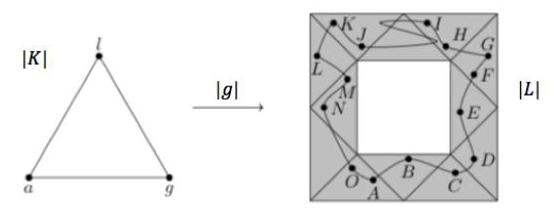
\includegraphics[width=0.6\textwidth]{images/Ch5_no_simplicial_map.jpg}
\end{center}
where \(\left| g\right| \left( a\right) = A\), \(\left| g\right| \left( g\right) = G\) and \(\left| g\right| \left( l\right) = L\). It is clear that we cannot find a 
simplicial map $\gamma: K \to L$ such that $|\gamma| = |g|$, since (for instance) the $1$-simplex $\Delta_{\{a,l\}}$ of $K$ does not lie in a single simplex $\Delta_{\sigma}$ of $L$. 

To remedy this, we subdivide \(K\) into smaller pieces as follows:
\begin{center}
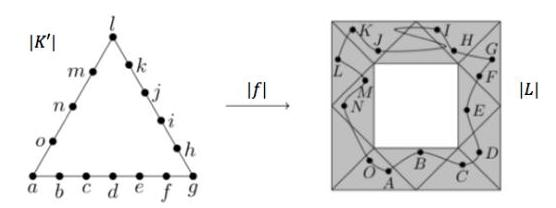
\includegraphics[width=0.6\textwidth]{images/Ch5_subdivide_map.jpg}
\end{center}
In this case, it is clear that 
one can define a simplicial map $f:K' \to L$ such that
\(\left| f\right|  : \left| {K}^{\prime }\right|  \rightarrow  \left| L\right|\) is our original map on the topological spaces.
\end{example}

\begin{example} [Barycentric Subdivision] One typical subdivision is the \emph{barycentric subdivision}. Namely, for each simplicial complex $K$, we add extra vertices, which corresponds to the barycenters of the topological realization of $K$. One example of such subdivision is given below:
\begin{center}
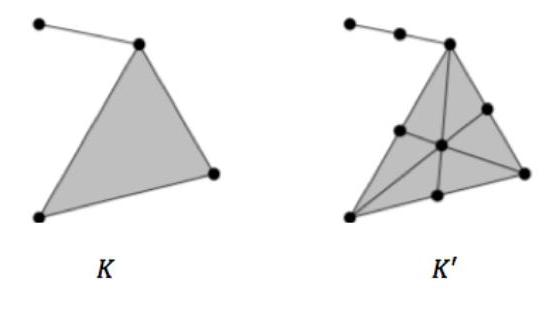
\includegraphics[width=0.5\textwidth]{images/Ch5_barycentric.jpg}
\end{center}
\end{example}

\begin{remark} Suppose we have a metric on \(\left| K\right|\). By subdivision, we can consider \(\left| {K}^{\prime }\right|\) such that for any \({\sigma }^{\prime } \in  {\sum }_{{K}^{\prime }}\), any two points in \({\Delta }_{{\sigma }^{\prime }}\) has a smaller distance.
\end{remark}

The following result gives a criterion for the existence of a simplicial approximation for a mapping between topological realizations. For this we recall the notion of star at a vertex \(v\) of $K$:
\[
\operatorname{star}\left( v\right)  = \mathop{\bigcup }\limits_{{v \in  \sigma }}{\sigma }^{ \circ  }.
\]

\begin{proposition} \label{prop:simplicial_approx} Let \(f : \left| K\right|  \rightarrow  \left| L\right|\) be a continuous mapping. Suppose that for each \(v \in  {V}_{K}\), there exists \(g\left( v\right)  \in  {V}_{L}\) such that
\[
f\left( {{\operatorname{st}}_{K}\left( v\right) }\right)  \subseteq  {\operatorname{st}}_{L}\left( {g\left( v\right) }\right)
\]
then the mapping \(g : {V}_{K} \rightarrow  {V}_{K}\) gives \(\left| g\right|  \simeq  f\). In such a case, \(g\) is called a {\bf simplicial approximation} to \(f\).
\end{proposition}

\begin{example} 
Let $K$ is as given below:
\begin{center}
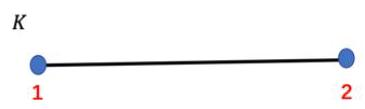
\includegraphics[width=0.3\textwidth]{images/Ch5_line_K.jpg}
\end{center}
If the map $f:|K| \to |L|$ is given by:
\begin{center}
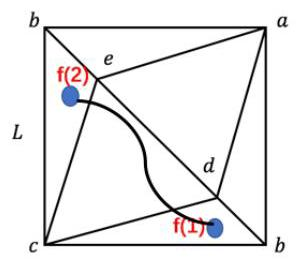
\includegraphics[width=0.4\textwidth]{images/Ch5_no_simp_K.jpg}
\end{center}
\hspace*{3em} 
The hypothesis of \autoref{prop:simplicial_approx} is not satisfied, so we cannot apply this proposition to construct a simplicial map $g: K \to L$ such that $|g| \simeq f$ (and indeed there is no such $g$).

However, if we subdivide $K$ into smaller parts (5 in the picture below): 
\begin{center}
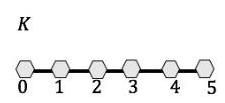
\includegraphics[width=0.4\textwidth]{images/Ch5_5_segments.jpg}
\end{center}
and $f:|K| \to |L|$ is given by:
\begin{center}
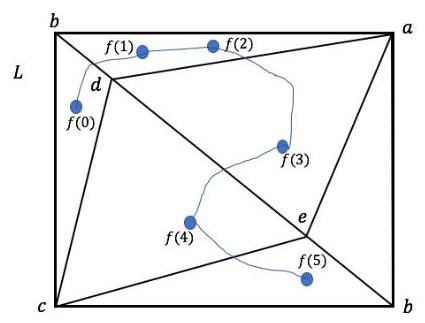
\includegraphics[width=0.4\textwidth]{images/Ch5_example_simplicial_approx.jpg}
\end{center}
then \autoref{prop:simplicial_approx} is satisfied. In such a case, 
we can take a simplicial approximation \(g\) by
\[
g\left( 0\right)  = b, g\left( 1\right)  = g\left( 2\right)  = d, g\left( 3\right)  = e, g\left( 4\right)  = c, g\left( 5\right)  = b.
\]
\end{example}

\begin{proof} We first show a statement: Suppose that \(\sigma  = \left\{  {{v}_{0}, \ldots, {v}_{n}}\right\}   \in  \sum \left( K\right)\), and \(x \in\) inside \(\left( \sigma \right)  \subseteq  \left| K\right|\). If \(f\left( x\right)  \in  \left| L\right|\) lies in the inside of the (unique) simplex \(\tau  \in  {\sum }_{L}\), (i.e., \(f\left( x\right)\) can uniquely be expressed as \(\mathop{\sum }\limits_{{{u}_{i} \in  \tau }}{\beta }_{i}{u}_{i}\), such that \({\beta }_{i} > 0, \forall i\) and \(\left. {\mathop{\sum }\limits_{i}{\beta }_{i} = 1}\right)\) then \(g\left( {v}_{0}\right), \ldots, g\left( {v}_{n}\right)\) are vertices of \(\tau\).

By definition of inside \(\left( \sigma \right), x = \mathop{\sum }\limits_{{i = 0}}^{n}{\alpha }_{i}{v}_{i}\) with \({\alpha }_{i} > 0\) and \(\mathop{\sum }\limits_{{i = 1}}^{n}{\alpha }_{i} = 1\). Therefore, \(x \in  {\operatorname{st}}_{K}\left( {v}_{i}\right)\) for \(i = 1, \ldots, n\), where

\[
{\operatorname{st}}_{K}\left( {v}_{i}\right)  \mathrel{\text{ := }} \left\{  {a{v}_{i} + \mathop{\sum }\limits_{{j = 1}}^{m}{b}_{j}{w}_{j} \mid  a > 0, {b}_{j} > 0, a + \mathop{\sum }\limits_{{j = 1}}^{m}{b}_{j} = 1, \left\{  {{v}_{i}, {w}_{1}, \ldots, {w}_{m}}\right\}   \in  {\sum }_{K}}\right\} .
\]

Therefore, \(f\left( x\right)  \in  \operatorname{int}\left( {{\operatorname{st}}_{K}\left( {v}_{i}\right) }\right)  \subseteq  {\operatorname{st}}_{L}\left( {g\left( {v}_{i}\right) }\right)\), which follows that

\[
f\left( x\right)  = {ag}\left( {v}_{i}\right)  + \mathop{\sum }\limits_{{j = 1}}^{m}{b}_{j}{u}_{j}, \text{ where }a > 0, {b}_{j} > 0, a + \mathop{\sum }\limits_{{j = 1}}^{m}{b}_{j} = 1, \left\{  {g\left( {v}_{i}\right), {u}_{1}, \ldots, {u}_{m}}\right\}   \in  {\sum }_{L}
\]

Comparing the above formula with our hypothesis on \(f\left( x\right), g\left( {v}_{i}\right)\) is a vertex of the simplex \(\tau, i = 1, \ldots, n\). Moreover, \(\left\{  {g\left( {v}_{0}\right), \ldots, g\left( {v}_{n}\right) }\right\}\) is a subset of \(\tau\), which is a face of \(\tau\), and therefore \(\left\{  {g\left( {v}_{0}\right), \ldots, g\left( {v}_{n}\right) }\right\}   \in  {\sum }_{L}\).

\begin{itemize}
\item Therefore, the mapping \(g : K \rightarrow  L\) maps simplicies to simplicies, which is a simplicial mapping. We can construct a homotopy between \(f\) and \(\left| g\right|\) as follows: Consider any \(x \in  \left| K\right|\), and let \(\tau  \in  {\sum }_{L}\) be such that \(f\left( x\right)  \in  \operatorname{inside}\left( \tau \right)\). We write \(x = \mathop{\sum }\limits_{{i = 0}}^{n}{\lambda }_{i}{v}_{i}\) for some \(\left\{  {{v}_{0}, \ldots, {v}_{n}}\right\}   \in  {\sum }_{K}\) and \({\lambda }_{i} > 0, \mathop{\sum }\limits_{{i = 1}}^{n}{\lambda }_{i} = 1\). Applying our claim, 
\end{itemize}

\[
\left| g\right| \left( x\right)  = \mathop{\sum }\limits_{{i = 0}}^{n}{\lambda }_{i}g\left( {v}_{i}\right), 
\]

where \(g\left( {v}_{0}\right), \ldots, g\left( {v}_{n}\right)\) are all vertices of \(\tau\).

We can directly construct a homotopy between \(f\) and \(\left| g\right|\). Before that, we need some reformulations. Since \(f\left( x\right)  \in  \operatorname{inside}\left( \tau \right)\), we let \(f\left( x\right)  = \mathop{\sum }\limits_{{i = 0}}^{m}{\mu }_{i}{\tau }_{i}\). Since \(\left| g\right| \left( x\right)  =\)  \(\mathop{\sum }\limits_{{i = 0}}^{n}{\lambda }_{i}g\left( {v}_{i}\right)  \in  \operatorname{inside}\left( \tau \right)\), we rewrite \(\left| g\right| \left( x\right)  = \mathop{\sum }\limits_{{i = 0}}^{m}{\lambda }_{i}^{\prime }{\tau }_{i}\). (by adding some \({\lambda }_{i}^{\prime } \mathrel{\text{ := }} 0\) if necessary) We define the map

\[
H : \;\left| K\right|  \times  I \rightarrow  \left| L\right|
\]

\[
\text{ with }\left( {x, t}\right)  \mapsto  \mathop{\sum }\limits_{{i = 0}}^{m}t{\lambda }_{i}^{\prime } + \left( {1 - t}\right) {\mu }_{i}
\]

which follows that \(f \simeq  \left| g\right|\).
\end{proof}

\begin{theorem} \label{thm:simplicial_approx}[Simplicial Approximation Theorem] Let \(K, L\) be simplicial complexes with \({V}_{K}\) finite, and \(f : \left| K\right|  \rightarrow  \left| L\right|\) be continuous. Then there exists a subdivision \(\left| {K}^{\prime }\right|\) of \(\left| K\right|\) together with a simplicial map \(g\) such that \(\left| g\right|  \simeq  f\).

Here the way for constructing subdivision \(\left| {K}^{\prime }\right|\) is as follows. There exists a constant \(\delta  > 0\). As long as the coarseness of \({K}^{\prime }\) is less than \(\delta\), our constructed subdivision satisfies the condition.
\end{theorem}


Proof. The sets \(\left\{  {{\operatorname{st}}_{L}\left( w\right)  \mid  w \in  V\left( L\right) }\right\}\) forms an open cover of \(\left| L\right|\), which implies \(\left\{  {{f}^{-1}\left( {{\operatorname{st}}_{L}\left( w\right) }\right) }\right\}\) forms an open cover of \(\left| K\right|\). By compactness, there exists a finite subcover of \(\left| K\right|\), denoted as

\[
\left| K\right|  \subseteq  \mathop{\bigcup }\limits_{{i = 1}}^{n}{f}^{-1}\left( {{\operatorname{st}}_{L}\left( {w}_{i}\right) }\right)
\]

There exists a small number \(\delta  > 0\) such that for any \(x, y \in  \left| K\right|\) with \(d\left( {x, y}\right)  < \delta\), \(x, y \in  {f}^{-1}\left( {{\operatorname{st}}_{L}\left( {w}_{i}\right) }\right)\) for some \(i\). Then we construct a simplicial subdivision \(\left| {K}^{\prime }\right|\) of \(\left| K\right|\) with coarseness less than \(\delta\), i.e., \(\forall x, y \in  {\operatorname{st}}_{{K}^{\prime }}\left( v\right), d\left( {x, y}\right)  < \delta\).

Therefore, \({\operatorname{st}}_{{K}^{\prime }}\left( v\right)  \subseteq  {f}^{-1}\left( {{\operatorname{st}}_{L}\left( {w}_{i}\right) }\right)\) for any \(v \in  V\left( K\right)\) and some \({w}_{i} \in  V\left( L\right)\), i.e., \(f\left( {{\operatorname{st}}_{{K}^{\prime }}\left( v\right) }\right)  \subseteq\)  \({\operatorname{st}}_{L}\left( {w}_{i}\right)\).


\chapter{Some Group Theory}

Group is a highlight of our course, which interwises topology and algebra. I assume that most students have learnt abstract algebra course MAT3004, and encourage those without this knowledge to read the notes for group posted on blackboard.

\section*{10.6. Wednesday for MAT4002}

\section*{10.6.1. Reviewing On Groups}

\begin{itemize}
\item Example 10.4 Let \({D}_{2n}\) be the regular polygon \(P\) with \({2n}\) sides in \({\mathbb{R}}^{2}\) , centered at the origin. It’s clear that \({D}_{2n}\) is invariant with \({2n}\) rotations, or with 2 reflections. Let \(a\) denote the rotation of \({D}_{2n}\) clockwise by degree \(\pi /n\) , and \(b\) denote the reflection over lines through the origin.
\end{itemize}

As a result, \(\left\{  {e,a,{a}^{2},\ldots ,{a}^{n - 1}}\right\}\) forms a group; and \(\{ e,b\}\) forms a group.

Therefore, all elements of \({D}_{g}\) can be obtained by \({a}^{i}{b}^{j},0 \leq  i \leq  3,0 \leq  j \leq  1\) .

Any finite operations of rotation (the rotation degree is a multiple of \(\pi /n\) ) and reflection can be represented as \({a}^{i}{b}^{j}\) .

Geometrically, we can check that \({ba} = {a}^{n - 1}b\) .

Definition 10.7 [Product Group] Let \(G,H\) be two groups. The product group \(\left( {G \times  H, * }\right)\) is defined as

\[
G \times  H = \{ \left( {g,h}\right)  \mid  g \in  G,h \in  H\}
\]

\[
\text{ with }\left( {{g}_{1},{h}_{1}}\right)  * \left( {{g}_{2},{h}_{2}}\right)  = \left( {{g}_{1}{g}_{2},{h}_{1}{h}_{2}}\right)
\]

For example, \(\left( {\mathbb{R} \times  \mathbb{R}, + }\right)  = \{ \left( {x,y}\right)  \mid  x,y \in  \mathbb{R}\}\) coincides with the usual \({\mathbb{R}}^{2}\) , where

\[
\left( {x,y}\right)  * \left( {{x}^{\prime },{y}^{\prime }}\right)  = \left( {x + {x}^{\prime },y + {y}^{\prime }}\right)
\]

Definition 10.8 A map between two groups \(\phi  : G \rightarrow  H\) is a homomorphism if

\[
\phi \left( {{g}_{1} * {g}_{2}}\right)  = \phi \left( {g}_{1}\right)  * \phi \left( {g}_{2}\right)
\]

In other words, a homomorphism is a map preserving multiplications of groups.

Follow the similar idea as in MAT3040 knowledge, if \(\phi  : G \rightarrow  H\) is a homomorphism, then \(\phi \left( {e}_{G}\right)  = {e}_{H}\) .

\begin{itemize}
\item Example 10.5 Let \(G = \left( {\mathbb{R},+,0}\right)\) , and \(H = \left\{  {{H}_{2},*,{I}_{2}}\right\}\) , with \({H}_{2}\) of the form
\end{itemize}

\[
{H}_{2} = \left\{  {\left. \left( \begin{array}{ll} 1 & x \\  0 & 1 \end{array}\right) \right| \;x \in  \mathbb{R}}\right\}
\]

Define a mapping

\[
\phi  : \;G \rightarrow  H
\]

\[
\text{ with }x \mapsto  \left( \begin{array}{ll} 1 & x \\  0 & 1 \end{array}\right)
\]

Then \(\phi\) is a homorphism:

\[
\phi \left( {x{ * }_{\mathbb{R}}y}\right)  = \phi \left( {x + y}\right)
\]

\[
= \left( \begin{matrix} 1 & x + y \\  0 & 1 \end{matrix}\right)
\]

\[
= \left( \begin{array}{ll} 1 & x \\  0 & 1 \end{array}\right) \left( \begin{array}{ll} 1 & y \\  0 & 1 \end{array}\right)
\]

\[
= \phi \left( x\right)  * {H}_{2}\phi \left( y\right)
\]

Definition 10.9 [Isomorphism] A homomorphism \(\phi  : G \rightarrow  H\) is an isomorphism if \(\phi\) is bijective. The isomorphism between \(G\) and \(H\) is denoted as \(G \cong  H\) .

Actually, a group can be represented as a Cayley Table:

\begin{center}
\adjustbox{max width=\textwidth}{
\begin{tabular}{|c|c|c|c|c|c|}
\hline
\multirow{5}{*}{\(G =\)} & 0 & \({g}_{1}\) & \({g}_{2}\) & ... & \({g}_{n}\) \\
\cline{2-6}
 & \({g}_{1}\) & \({g}_{1} \circ  {g}_{1}\) & \({g}_{1} \circ  {g}_{2}\) & ... & \({g}_{1} \circ  {g}_{n}\) \\
\cline{2-6}
 & \({g}_{2}\) & \({g}_{2} \circ  {g}_{1}\) & \({g}_{2} \circ  {g}_{2}\) & ... & \({g}_{2} \circ  {g}_{n}\) / \\
\cline{2-6}
 & \(\vdots\) & \(\vdots\) & ... & \(\vdots\) & \(\vdots\) \\
\cline{2-6}
 & \({g}_{n}\) & \({g}_{n} \circ  {g}_{1}\) & \({g}_{n} \circ  {g}_{2}\) & ... & \({g}_{n} \circ  {g}_{n}\) \\
\cline{1-6}
\hline
\end{tabular}
}
\end{center}

\begin{center}
\adjustbox{max width=\textwidth}{
\begin{tabular}{|c|c|c|c|c|c|}
\hline
\multirow{5}{*}{\(H =\)} & 0 & \({h}_{1}\) & \({h}_{2}\) & ... & \({h}_{n}\) \\
\cline{2-6}
 & \({h}_{1}\) & \({h}_{1} \circ  {h}_{1}\) & \({h}_{1} \circ  {h}_{2}\) & ... & \({h}_{1} \circ  {h}_{n}\) \\
\cline{2-6}
 & \({h}_{2}\) & \({h}_{2} \circ  {h}_{1}\) & \({h}_{2} \circ  {h}_{2}\) & ... & \({h}_{2} \circ  {h}_{n}\) \\
\cline{2-6}
 & \(\vdots\) & \(\vdots\) & ... & \(\vdots\) & \(\vdots\) \\
\cline{2-6}
 & \({h}_{n}\) & \({h}_{n} \circ  {h}_{1}\) & \({h}_{n} \circ  {h}_{2}\) & ... & \({h}_{n} \circ  {h}_{n}\) \\
\cline{1-6}
\hline
\end{tabular}
}
\end{center}

The groups \(G \cong  H\) if and only if we can find a bijective \(\phi  : G \rightarrow  H\) such that, the Cayley

Table of \(\left( {H, \circ  }\right)\) can be generated from the Cayley Table of \(\left( {G, \circ  }\right)\) by replacing each entry of \(G\) with its image under \(\phi\) .

\section*{10.6.2. Free Groups}

10.10 . Let \(S\) be a (finite) set, which is considered as an "alphabet".

\begin{itemize}
\item Define another set \({S}^{-1} \mathrel{\text{ := }} \left\{  {{x}^{-1} \in  x \in  S}\right\}\) . We insist that \(S \cap  {S}^{-1} = \varnothing\) .
\end{itemize}

\begin{itemize}
\item A word in \(S\) is a finite sequence \(w = {w}_{1}\cdots {w}_{m}\) , where \(m \in  {\mathbb{N}}^{ + } \cup  \{ 0\}\) , and each \({w}_{i} =  \in   \cup  {S}^{-1}\) . In particular, when \(m = 0\) , we view \(w\) as the empty sequence, denoted as \(\varnothing\) .
\end{itemize}

\begin{itemize}
\item The concatenation of two words \({x}_{1}\cdots {x}_{m}\) and \({y}_{1}\cdots {y}_{n}\) is the word \({x}_{1}\cdots {x}_{m}{y}_{1}\cdots {y}_{n}\)
\end{itemize}

\begin{itemize}
\item Two words \(w,{w}^{\prime }\) are equivalent, denoted as \(w \sim  {w}^{\prime }\) , if there are words \({w}_{1},\ldots ,{w}_{n}\) and \(w = {w}_{1},{w}^{\prime } = {w}_{n}\) such that
\end{itemize}

\[
{w}_{i} = \cdots {y}_{1}x{x}^{-1}{y}_{2}\cdots ,\;{w}_{i + 1} = \cdots {y}_{1}{y}_{2}\cdots
\]

or

\[
{w}_{i} = \cdots {y}_{1}{y}_{2}\cdots ,\;{w}_{i + 1} = \cdots {y}_{1}x{x}^{-1}{y}_{2}\cdots
\]

for some \(x \in  S \cup  {S}^{-1}\) .

\begin{itemize}
\item Example 10.6 For example, \(S = \{ a,b\}\) and \({S}^{-1} = \left\{  {{a}^{-1}{b}^{-1}}\right\}\) and
\end{itemize}

\[
w = {aaba}{b}^{-1}{b}^{-1}{a}^{-1}{abaab}{b}^{-1}a
\]

\[
{w}^{\prime } = {aaba}{b}^{-1}{b}^{-1}{a}^{-1}{abaaa}
\]

Here \(w\) and \({w}^{\prime }\) differs by \(b{b}^{-1}\) . Therefore, \(w \sim  {w}^{\prime }\) , and \(w\) is said to be a elementary expansion of \({w}^{\prime }\) .

We insist that \({\left( {s}^{-1}\right) }^{-1} = s,\forall {s}^{-1} \in  {S}^{-1}\) , since otherwise for \(x = {s}^{-1} \in  {S}^{-1}\) , we cannot define \({\left( {s}^{-1}\right) }^{-1}\) .

Moreover, for

\[
w = {aaba}{b}^{-1}{b}^{-1}{a}^{-1}{abaab}{b}^{-1}a
\]

\[
{w}^{\prime \prime } = {aaba}{b}^{-1}{b}^{-1}{baab}{b}^{-1}a,
\]

\(w\) and \({w}^{\prime \prime }\) differs by \({a}^{-1}a\) , i.e., \({a}^{-1}{\left( {a}^{-1}\right) }^{-1}\) , and therefore \(w \sim  {w}^{\prime \prime }\) .

Definition 10.11 [Free Group] The free group \(F\left( S\right)\) is defined to be the equivalence class of words, i.e.,

\[
\left\lbrack  w\right\rbrack   \mathrel{\text{ := }} \left\{  {{w}^{\prime }\text{ is a word in }S \mid  w \sim  {w}^{\prime }}\right\}   \in  F\left( S\right)
\]

\(F\left( S\right)\) is indeed a group:

\begin{itemize}
\item \(\left\lbrack  w\right\rbrack   * \left\lbrack  {w}^{\prime }\right\rbrack   = \left\lbrack  {w{w}^{\prime }}\right\rbrack\) (concatenation) check \({w}_{1} \sim  {w}_{2},{u}_{1} \sim  {u}_{2}\) implies \({w}_{1}{u}_{1} \sim\)  \({w}_{2}{u}_{2}\)
\end{itemize}

\begin{itemize}
\item Identity element: \(e = \left\lbrack  \varnothing \right\rbrack\)
\end{itemize}

\begin{itemize}
\item Inverse element: \({\left\lbrack  {x}_{1}\cdots {x}_{n}\right\rbrack  }^{-1} = \left\lbrack  {{x}_{n}^{-1}\cdots {x}_{1}^{-1}}\right\rbrack\)
\end{itemize}

\begin{itemize}
\item Example 10.7 Let \(S = \{ a\}\) and \({S}^{-1} = \left\{  {a}^{-1}\right\}\) . Any word \(w\) has the form
\end{itemize}

\[
w = a\cdots a{a}^{-1}\cdots {a}^{-1}a\cdots a{a}^{-1}\cdots {a}^{-1}\cdots
\]

In shorthand, we denote \(w\) as \(w = \cdots {a}^{p}{\left( {a}^{-1}\right) }^{q}{a}^{r}{\left( {a}^{-1}\right) }^{s}\cdots\) , and

\[
\left\lbrack  w\right\rbrack   = \left\lbrack  {\cdots {a}^{p}{\left( {a}^{-1}\right) }^{q}{a}^{r}{\left( {a}^{-1}\right) }^{s}\cdots }\right\rbrack   = \left\lbrack  {\cdots {a}^{p - 1}{\left( {a}^{-1}\right) }^{q - 1}{a}^{r}{\left( {a}^{-1}\right) }^{s}\cdots }\right\rbrack
\]

\[
= \left\lbrack  {\cdots {a}^{p - 1}{\left( {a}^{-1}\right) }^{q - 2}{a}^{r - 1}{\left( {a}^{-1}\right) }^{s}\cdots }\right\rbrack  ,
\]

e.g., we can always eliminate the adjacent terms \(a\) and \({a}^{-1}\) up to equivalence class. Therefore, \(F\left( S\right)  = \left\{  {\cdots ,\left\lbrack  {a}^{-2}\right\rbrack  ,\left\lbrack  {a}^{-1}\right\rbrack  ,\left\lbrack  \varnothing \right\rbrack  ,\left\lbrack  a\right\rbrack  ,\left\lbrack  {a}^{2}\right\rbrack  ,\cdots }\right\}\) .

It’s clear that \(F\left( S\right)  \cong  \mathbb{Z}\) , where the isomorphism \(\phi  : \mathbb{Z} \rightarrow  F\left( S\right)\) is \(\phi \left( n\right)  = \left\lbrack  {a}^{n}\right\rbrack\) .

\begin{itemize}
\item Example 10.8 Let \(S = \{ a,b\}\) and \({S}^{-1} = \left\{  {{a}^{-1},{b}^{-1}}\right\}\) . In this case, \(\left\lbrack  {ab}\right\rbrack   \neq  \left\lbrack  {ba}\right\rbrack\) , and \(\left\lbrack  {a{b}^{-1}{a}^{2}{b}^{2}{a}^{-2}b}\right\rbrack\) cannot be reduced further.
\end{itemize}

Since \(S\) is not an abelian group in such case, we imply \(F\left( S\right)  ≆ \mathbb{Z} \times  \mathbb{Z}\) .

\section*{10.6.3. Relations on Free Groups}

Definition 10.12 [Group With Relations] Let \(S\) be a set. A group with relations is written as

\[
G = \langle S \mid  R\left( S\right) \rangle
\]

where

\begin{itemize}
\item \(R\left( S\right)\) consists of elements in \(F\left( S\right)\)
\end{itemize}

\begin{itemize}
\item Every element in \(G\) can be written as the form \(\left\lbrack  w\right\rbrack   \in  F\left( S\right)\) , and we insist that \(\left\lbrack  w\right\rbrack   = \left\lbrack  {w}^{\prime }\right\rbrack\) in \(G\) if
\end{itemize}

\begin{itemize}
\item \(w\) and \({w}^{\prime }\) differ by some \(x{x}^{-1},x \in  S \cup  {S}^{-1}\) , or
\end{itemize}

\begin{itemize}
\item \(w\) and \({w}^{\prime }\) differ by some element \(z \in  R\left( S\right)\) , or its inverse.
\end{itemize}

\begin{itemize}
\item Example 10.9 Let \(G = \left\langle  {a,b \mid  {a}^{2},{b}^{2},{aba}{b}^{-1}{a}^{-1}{b}^{-1}}\right\rangle\) , we want to enumerate all possible elements in \(G\) . Obseve that
\end{itemize}

\[
\left\lbrack  {b}^{-1}\right\rbrack   = \left\lbrack  {{b}^{-1}{b}^{2}}\right\rbrack   = \left\lbrack  b\right\rbrack  ,\;\text{ similarly }\left\lbrack  {a}^{-1}\right\rbrack   = \left\lbrack  a\right\rbrack
\]

\[
\left\lbrack  {bab}\right\rbrack   = \left\lbrack  {{aba}{b}^{-1}{a}^{-1}{b}^{-1}{bab}}\right\rbrack   = \left\lbrack  {{aba}{b}^{-1}b}\right\rbrack   = \left\lbrack  {aba}\right\rbrack
\]

As a result,

\begin{itemize}
\item \(\left\lbrack  {a}^{-n}\right\rbrack   = \left\lbrack  {a}^{n}\right\rbrack\) and \(\left\lbrack  {b}^{-n}\right\rbrack   = \left\lbrack  {b}^{n}\right\rbrack\)
\end{itemize}

\begin{itemize}
\item \(\left\lbrack  {a}^{{2n} + 1}\right\rbrack   = \left\lbrack  a\right\rbrack  ,\left\lbrack  {b}^{{2n} + 1}\right\rbrack   = \left\lbrack  b\right\rbrack  ,\left\lbrack  {a}^{2n}\right\rbrack   = \left\lbrack  \varnothing \right\rbrack  ,\left\lbrack  {b}^{2n}\right\rbrack   = \left\lbrack  \varnothing \right\rbrack\)
\end{itemize}

\begin{itemize}
\item For another type of element of \(G\) , it must be of the form \(\left\lbrack  {\cdot {abababab}\cdots }\right\rbrack\) .
\end{itemize}

Each aba can be changed into \({bab}\) , and finally it will be reduced into the form \(\left\lbrack  {ab}\right\rbrack\) . Therefore, the elements in \(G\) are

\[
\left\lbrack  \varnothing \right\rbrack  ,\left\lbrack  a\right\rbrack  ,\left\lbrack  b\right\rbrack  ,\left\lbrack  {ab}\right\rbrack  ,\left\lbrack  {ba}\right\rbrack  ,\left\lbrack  {aba}\right\rbrack
\]

In fact, \(G \cong  {S}_{3}\) .

\section*{11.3. Monday for MAT4002}

Reviewing. Consider the group with presentation \(\langle S \mid  R\left( S\right) \rangle\) .

1. The elements in \(S\) are generators that have studied in abstract algebra

2. The "relations" of this group are given by the equalities on hte right-hand side, e.g., the dihedral group is defined as

\[
\left\langle  {a,b \mid  {a}^{n} = e,{b}^{2} = e,{bab} = {a}^{-1}}\right\rangle
\]

Sometimes we also simplify the equality \(\times   = e\) as \(\times\) , e.g., the dihedral group can be re-written as

\[
\left\langle  {a,b \mid  {a}^{n},{b}^{2},{bab} = {a}^{-1}}\right\rangle
\]

\section*{Example 11.4 Consider}

\[
G =  < a,b \mid  {a}^{2},{b}^{2},{aba}{b}^{-1}{a}^{-1}{b}^{-1} >  \mathrel{\text{ := }}  < a,b \mid  {a}^{2},{b}^{2},{aba} = {bab} >  = \{ e,a,b,{ab},{ba},{aba}\}
\]

It’s isomorphic to \({S}^{3}\) , and the shape of \({S}^{3}\) is illustrated in Fig.(11.1)

\begin{center}
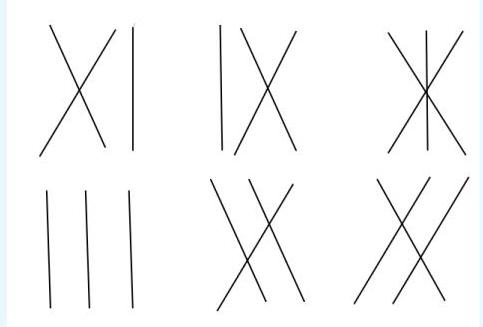
\includegraphics[max width=0.4\textwidth]{images/bo_d2bcsrref24c73avs720_107_737_1365_483_327_0.jpg}
\end{center}
\hspace*{3em} 

Figure 11.1: Illustration of group \({S}^{3}\)

More precisely, the isomorphism is given by:

\[
\phi  : \;{S}_{3} \rightarrow  G
\]

\[
\text{ with }X \mid   \mapsto  a,\; \mid  X \mapsto  b
\]

\begin{itemize}
\item Example 11.5 Consider \({G}_{2} =  < a,b \mid  {ab} = {ba} >\) and any word, which can be expressed as \(\cdots {a}^{s}{b}^{t}{a}^{u}{b}^{v}\cdots\)
\end{itemize}

\begin{itemize}
\item If \(s \in  \mathbb{N}\) , we write \({a}^{s} \mathrel{\text{ := }} \underset{s\text{ times }}{\underbrace{a\cdots a}}\)
\end{itemize}

\begin{itemize}
\item If \(s \in   - \mathbb{N}\) , we write \({a}^{s} \mathrel{\text{ := }} \underset{-s\text{ times }}{\underbrace{\left( {a}^{-1}\right) \cdots \left( {a}^{-1}\right) }}\)
\end{itemize}

\begin{itemize}
\item For the word with the form \(a\cdots b\cdots {ba}\cdots a\) , we can always push \(a\) into the leftmost using the relation \({ab} = {ba}\)
\end{itemize}

\begin{itemize}
\item For the word with the form \(a\cdots {ab}\cdots b{a}^{-1}\) , we can always push \({a}^{-1}\) into the leftmost using the relation \(b{a}^{-1} = {a}^{-1}b\) .
\end{itemize}

Therefore, all elements in \({G}_{2}\) are of the form \({a}^{p}{b}^{q},p,q \in  \mathbb{Z}\) , and we have the relation

\[
\left( {{a}^{{p}_{1}}{b}^{{q}_{1}}}\right) \left( {{a}^{{p}_{2}}{b}^{{q}_{2}}}\right)  = {a}^{{p}_{1} + {p}_{2}}{b}^{{q}_{1} + {q}_{2}}.
\]

Therefore, \({G}_{2} \cong  \mathbb{Z} \times  \mathbb{Z}\) , where the isomorphism is given by:

\[
\phi  : \;\mathbb{Z} \times  \mathbb{Z} \rightarrow  {G}_{2}
\]

\[
\text{ with }\left( {p,q}\right)  \mapsto  {a}^{p}{b}^{q}
\]

\begin{itemize}
\item Example 11.6
\end{itemize}

\[
{G}_{3} = \left\langle  {a \mid  {a}^{5}}\right\rangle   = \left\{  {1,a,{a}^{2},\ldots ,{a}^{4}}\right\}
\]

It’s clear that \({G}_{3} \cong  \mathbb{Z}/5\mathbb{Z}\) , where the isomorphism is given by:

\[
\phi  : \;\mathbb{Z}/5\mathbb{Z} \rightarrow  {G}_{3}
\]

\[
\text{ with }m + 5\mathbb{Z} \mapsto  {a}^{m}
\]

\section*{11.3.1. Cayley Graph for finitely presented groups}

Graphs have strong connection with groups. Here we introduce a way of building graphs using groups, and the graphs are known as Cayley graphs. They describe many properties of the group in a topological way.

Definition 11.5 [Oriented Graph] An oriented graph \(T\) is specified by

1. A countable or finite set \(V\) , known as vertices

2. A countable or finite set \(E\) , known as edges

3. A function \(\delta  : E \rightarrow  V \times  V\) given by

\[
\delta \left( e\right)  = \left( {\ell \left( e\right) ,\tau \left( e\right) }\right)
\]

where \(\ell \left( e\right)\) denotes the initial vertex and \(\tau \left( e\right)\) denotes the terminal vertex.

For example, let

\begin{itemize}
\item \(V = \{ a,b,c\}\)
\end{itemize}

\begin{itemize}
\item \(E = \left\{  {{e}_{1},{e}_{2},{e}_{3},{e}_{4}}\right\}\)
\end{itemize}

\begin{itemize}
\item \(\delta \left( {e}_{1}\right)  = \left( {a,a}\right) ,\delta \left( {e}_{2}\right)  = \left( {b,c}\right) ,\delta \left( {e}_{3}\right)  = \left( {a,c}\right) ,\delta \left( {e}_{4}\right)  = \left( {b,c}\right)\)
\end{itemize}

\begin{center}
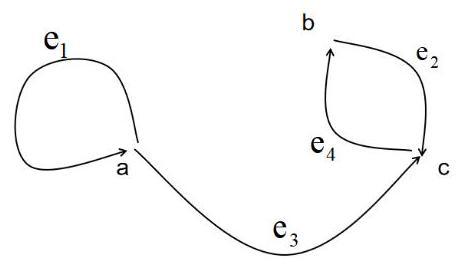
\includegraphics[max width=0.3\textwidth]{images/bo_d2bcsrref24c73avs720_109_740_1525_457_264_0.jpg}
\end{center}
\hspace*{3em} 

Figure 11.2: Illustration of example oriented graph

The resulted graph is plotted in Fig.(11.2)

Definition 11.6 [Cayley graph] Let \(G = \langle S \mid  R\left( S\right) \rangle\) with \(\left| S\right|  < \infty\) . The Cayley graph associated to \(G\) is an oriented graph with

1. The vertex set \(G\)

2. The edge set \(E \mathrel{\text{ := }} G \times  S\)

3. The function \(\ell  : E \rightarrow  V \times  V\) is given by:

\(\ell  : \;G \times  S \rightarrow  G \times  G\)

with \(\left( {g,s}\right)  \mapsto  \left( {g,g \cdot  s}\right)\)

In particular, we link two elements in \(G\) if they differ by a generator rightside.

1. The Cayley graph for \(G = \langle a\rangle \left( { \cong  \mathbb{Z}}\right)\) is shown in Fig.(11.3):

\begin{center}
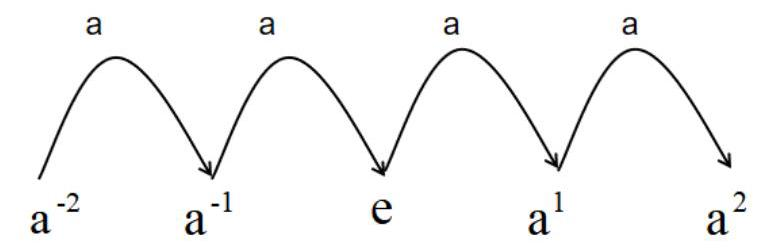
\includegraphics[max width=0.6\textwidth]{images/bo_d2bcsrref24c73avs720_110_448_1055_769_250_0.jpg}
\end{center}
\hspace*{3em} 

Figure 11.3: Illustration of Cayley Graph \(\langle a\rangle\)

2. The Cayley graph for \(G = \left\langle  {a \mid  {a}^{3}}\right\rangle\) is shown in Fig.(11.4):

\begin{center}
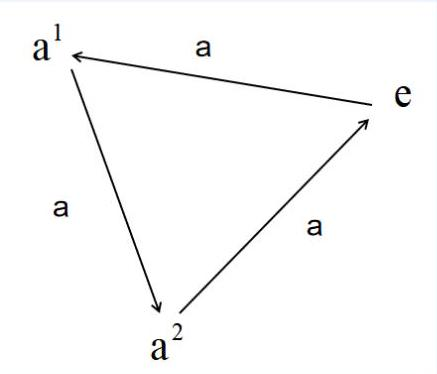
\includegraphics[max width=0.3\textwidth]{images/bo_d2bcsrref24c73avs720_110_618_1541_437_374_0.jpg}
\end{center}
\hspace*{3em} 

Figure 11.4: Illustration of Cayley Graph \(\left\langle  {a \mid  {a}^{3}}\right\rangle\)

3. The Cayley graph for \(G = \left\langle  {a,b \mid  {a}^{2},{b}^{2},{aba} = {bab}}\right\rangle\) is shown in Fig.(11.12):

\begin{center}
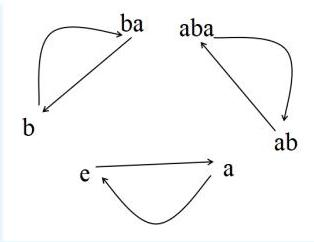
\includegraphics[max width=0.2\textwidth]{images/bo_d2bcsrref24c73avs720_111_811_303_314_242_0.jpg}
\end{center}
\hspace*{3em} 

Figure 11.5: Illustration of Cayley Graph \(\left\langle  {a,b \mid  {a}^{2},{b}^{2},{aba} = {bab}}\right\rangle\)

4. The Cayley graph for \(G = \langle a,b \mid  {ab} = {ba}\rangle\) is shown in Fig.(11.6):

\begin{center}
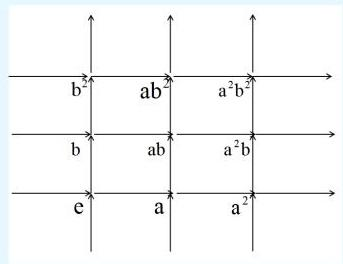
\includegraphics[max width=0.2\textwidth]{images/bo_d2bcsrref24c73avs720_111_805_742_343_264_0.jpg}
\end{center}
\hspace*{3em} 

Figure 11.6: Illustration of Cayley Graph \(\langle a,b \mid  {ab} = {ba}\rangle\)

5. The Cayley graph for \(G = \langle a,b\rangle\) is shown in Fig.(11.7):

\begin{center}
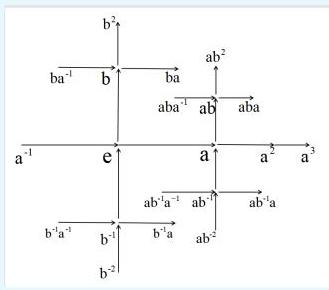
\includegraphics[max width=0.2\textwidth]{images/bo_d2bcsrref24c73avs720_111_809_1204_329_290_0.jpg}
\end{center}
\hspace*{3em} 

Figure 11.7: Illustration of Cayley Graph \(\langle a,b \mid  {ab} = {ba}\rangle\)

There could be different presentations \(\left\langle  {{S}_{1} \mid  R\left( {S}_{1}\right) }\right\rangle   \cong  \left\langle  {{S}_{2} \mid  R\left( {S}_{2}\right) }\right\rangle\) of the same group.

\chapter{Fundamental Group}

Motivation. The fundamental group connects topology and algebra together, by labelling a group to each topological space, which is known as fundamental group.

Why do we need algebra in topology. Consider the \({S}^{2}\) (2-shpere) and \({S}^{1} \times  {S}^{1}\)

(torus):

\begin{center}
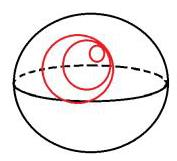
\includegraphics[max width=0.2\textwidth]{images/bo_d2bcsrref24c73avs720_112_711_510_177_161_0.jpg}
\end{center}
\hspace*{3em} 

Figure 11.8: Any loop in the sphere can be contracted into a point

\begin{center}
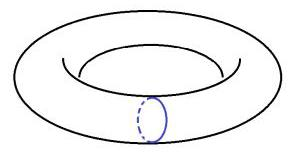
\includegraphics[max width=0.2\textwidth]{images/bo_d2bcsrref24c73avs720_112_656_964_289_152_0.jpg}
\end{center}
\hspace*{3em} 

Figure 11.9: Some loops in the torus cannot be contracted into a point

As can be seen from Fig.(11.8) and Fig.(11.9), any "loop" on a sphere can be contracted to a point, while some "loop" on a torus cannot. We need the algebra to describe this phenomena formally.

Definition 11.7 [loop] Let \(X\) be a topological space. A loop on \(X\) is a constant map \(\ell  : \left\lbrack  {0,1}\right\rbrack   \rightarrow  X\) such that \(\ell \left( 0\right)  = \ell \left( 1\right)\) .

We say \(\ell\) is based at \(b \in  X\) if \(\ell \left( 0\right)  = \ell \left( 1\right)  = b\) .

Definition 11.8 [composite loop] Suppose that \(\mathbf{u},\mathbf{v}\) are loops on \(X\) based at \(b \in  X\) . The composite loop \(u \cdot  v\) is given by

\[
u \cdot  v = \left\{  \begin{array}{rr} u\left( {2t}\right) , & \text{ if }0 \leq  t \leq  1/2 \\  v\left( {{2t} - 1}\right) , & \text{ if }1/2 \leq  t \leq  1 \end{array}\right.
\]

Definition 11.9 [fundamental group] The homotopy class of loops relative to \(\{ 0,1\}\) based at \(b \in  X\) forms a group. It is called the fundamental group of \(X\) based at \(b\) , denoted as \({\pi }_{1}\left( {X,b}\right)\) .

More precisely, let

\(\left\lbrack  \ell \right\rbrack   = \{ m \mid  m\) is a loop based at \(b\) that is homotopic to \(\ell\) , relative to \(\{ 0,1\} \}\) ,

and \({\pi }_{1}\left( {X,b}\right)  = \{ \left\lbrack  \ell \right\rbrack   \mid  \ell\) are loops based at \(b\}\) . The operation in \({\pi }_{1}\left( {X,b}\right)\) is defined as:

\[
\left\lbrack  \ell \right\rbrack   * \left\lbrack  {\ell }^{\prime }\right\rbrack   \mathrel{\text{ := }} \left\lbrack  {\ell  \cdot  {\ell }^{\prime }}\right\rbrack  ,\;\forall \left\lbrack  \ell \right\rbrack  ,\left\lbrack  {\ell }^{\prime }\right\rbrack   \in  {\pi }_{1}\left( {X,b}\right) .
\]

R Two paths \({\ell }_{1},{\ell }_{2} : \left\lbrack  {0,1}\right\rbrack   \rightarrow  X\) are homotopic relative to \(\{ 0,1\}\) if we can find \(H : \left\lbrack  {0,1}\right\rbrack   \times  \left\lbrack  {0,1}\right\rbrack   \rightarrow  X\) such that

\[
H\left( {t,0}\right)  = {\ell }_{1}\left( t\right) ,\;H\left( {t,1}\right)  = {\ell }_{2}\left( t\right)
\]

and

\[
H\left( {0,s}\right)  = {\ell }_{1}\left( 0\right)  = {\ell }_{2}\left( 0\right) ,\forall 0 \leq  s \leq  1,\;H\left( {1,s}\right)  = {\ell }_{1}\left( 1\right)  = {\ell }_{2}\left( 1\right) ,\forall 0 \leq  s \leq  1
\]

Counter example for homotopy but not relative to \(\{ 0,1\}\) :

\begin{center}
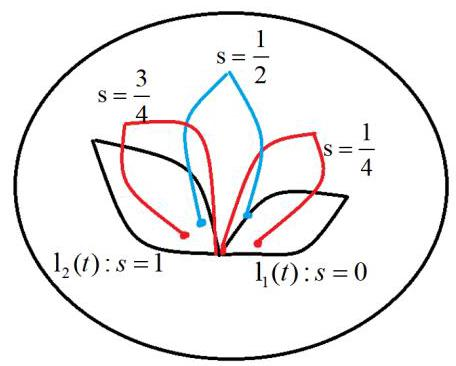
\includegraphics[max width=0.3\textwidth]{images/bo_d2bcsrref24c73avs720_113_744_1658_456_366_0.jpg}
\end{center}
\hspace*{3em} 

Figure 11.10: homotopy not relative to \(\{ 0,1\}\)

\section*{11.6. Wednesday for MAT4002}

\section*{11.6.1.The fundamental group}

Revewing. One example for Homotopy relative to \(\{ 0,1\}\) is illustrated in Fig.(11.4)

\begin{center}
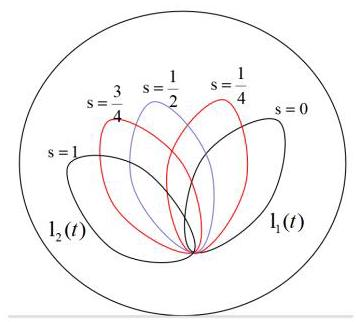
\includegraphics[max width=0.3\textwidth]{images/bo_d2bcsrref24c73avs720_114_646_571_356_322_0.jpg}
\end{center}
\hspace*{3em} 

Figure 11.11: Example of homotopy relative to \(\{ 0,1\}\)

It’s essential to study homotopy relative to \(\{ 0,1\}\) . For example, given a torus with a loop \({\ell }_{1}\left( t\right)\) and a base point \(b\) . We want to distinguish \({\ell }_{1}\left( t\right)\) and \({\ell }_{2}\left( t\right)\) as shown in Fig.(11.12):

\begin{center}
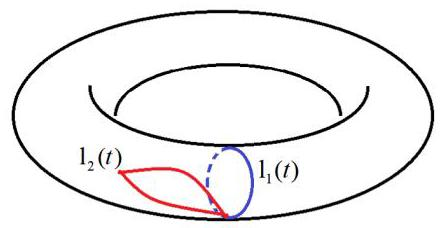
\includegraphics[max width=0.3\textwidth]{images/bo_d2bcsrref24c73avs720_114_596_1228_442_228_0.jpg}
\end{center}
\hspace*{3em} 

Figure 11.12: Two loops on a torus

Obviously there should be something different between \({\ell }_{1}\left( t\right)\) and \({\ell }_{2}\left( t\right)\) . "Relative to \(\{ 0,1\}\) is essential", sicne if we get rid of this condition, all loops are homotopic to the constant map \({c}_{b}\left( t\right)  = b\) . See the graphic illustration in Fig.(??):

\begin{center}
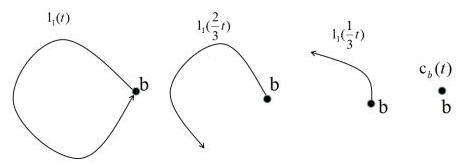
\includegraphics[max width=0.3\textwidth]{images/bo_d2bcsrref24c73avs720_114_591_1782_464_166_0.jpg}
\end{center}
\hspace*{3em} 

Figure 11.13: homotopy between any loop and constant map

In this case, \(\ell  \simeq  {c}_{b}\) for any loop \(\ell\) , there is only one trivial element \(\left\{  \left\lbrack  {c}_{b}\right\rbrack  \right\}\) in \({\pi }_{1}\left( {X,b}\right)\) .

That’s the reason why we define \({\pi }_{1}\left( {X,b}\right)\) as the collection of homotopy classes relative to \(\{ 0,1\}\) based at \(b\) in \(X\) .

Proposition 11.13 Let \(\left\lbrack  \cdot \right\rbrack\) denote the homotopy class of loops relative to \(\{ 0,1\}\) based at \(b\) , and define the operation

\[
\left\lbrack  \ell \right\rbrack   * \left\lbrack  {\ell }^{\prime }\right\rbrack   = \left\lbrack  {\ell  \cdot  {\ell }^{\prime }}\right\rbrack
\]

Then \(\left( {{\pi }_{1}\left( {X,b}\right) , * }\right)\) forms a group, where

\[
{\pi }_{1}\left( {X,b}\right)  \mathrel{\text{ := }} \{ \left\lbrack  \ell \right\rbrack   \mid  \ell  : \left\lbrack  {0,1}\right\rbrack   \rightarrow  X\text{ denotes loops based at }b\}
\]

Proof. 1. Well-definedness: Suppose that \(u \sim  {u}^{\prime }\) and \(v \sim  {v}^{\prime }\) , it suffices to show \(u \cdot  v \simeq\)  \({u}^{\prime } \cdot  {v}^{\prime }\) . Consider the given homotopies \(H : u \simeq  {u}^{\prime },K : v \simeq  {v}^{\prime }\) . Construct a new homotopy \(L : I \times  I \rightarrow  X\) by

\[
L\left( {t,s}\right)  = \left\{  \begin{array}{rr} H\left( {{2t},s}\right) , & 0 \leq  t \leq  1/2 \\  K\left( {{2t} - 1,s}\right) , & 1/2 \leq  t \leq  1 \end{array}\right.
\]

The diagram below explains the ideas for constructing \(L\) . The plane denote the set \(I \times  I\) , and the labels characterize the images of each point of \(I \times  I\) under \(L\) . Therefore, \(u \cdot  v \simeq  {u}^{\prime } \cdot  {v}^{\prime }\) .

\begin{center}
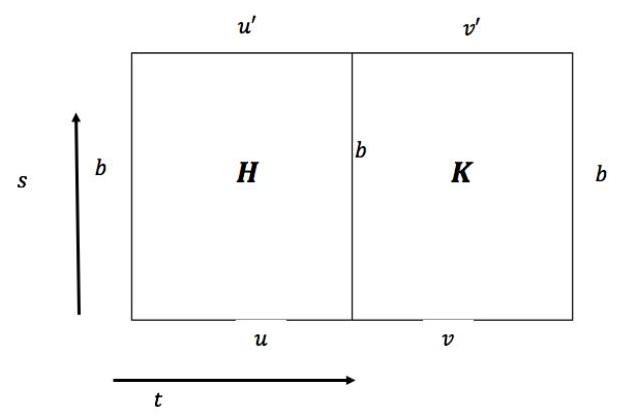
\includegraphics[max width=0.5\textwidth]{images/bo_d2bcsrref24c73avs720_115_639_1586_617_417_0.jpg}
\end{center}
\hspace*{3em} 

2. Associate: \(\left( {u \cdot  v}\right)  \cdot  w \simeq  u \cdot  \left( {v \cdot  w}\right)\)

Note that \(\left( {u \cdot  v}\right)  \cdot  w\) and \(u \cdot  \left( {v \cdot  w}\right)\) are essentially different loops. Although they go with the same path, they are with different speeds. Generally speaking, the loop \(\left( {u \cdot  v}\right)  \cdot  w\) travels \(u,v\) using \(1/4\) seconds, and \(w\) in \(1/2\) seconds; but the loop \(u \cdot  \left( {v \cdot  w}\right)\) travels \(u\) in \(1/2\) seconds, and then \(v,w\) in \(1/4\) seconds.

We want to construct a homotopy that describes the loop changes from \(u \cdot  \left( {v \cdot  w}\right)\) to \(\left( {u \cdot  v}\right)  \cdot  w\) . A graphic illustration is given below:

\begin{center}
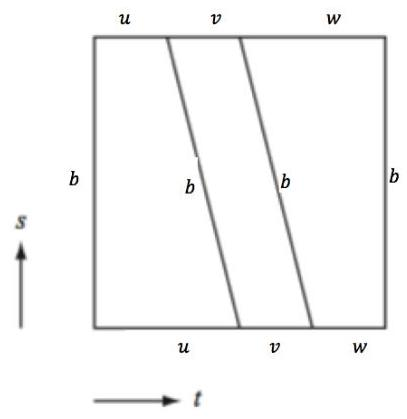
\includegraphics[max width=0.3\textwidth]{images/bo_d2bcsrref24c73avs720_116_621_761_407_419_0.jpg}
\end{center}
\hspace*{3em} 

An explicit homotopy \(H : I \times  I \rightarrow  X\) is given below:

\[
H\left( {t,s}\right)  = \left\{  \begin{matrix} u\left( {{4t}/\left( {2 - s}\right) }\right) , & 0 \leq  t \leq  1/2 - 1/{4s} \\  v\left( {{4t} - 2 + s}\right) , & 1/2 - 1/{4s} \leq  t \leq  3/4 - 1/{4s} \\  w\left( {{4t} - 3 + s/\left( {1 + s}\right) }\right) , & 3/4 - 1/{4s} \leq  t \leq  1 \end{matrix}\right.
\]

Therefore,

\[
\left\lbrack  u\right\rbrack   * \left( {\left\lbrack  v\right\rbrack   * \left\lbrack  w\right\rbrack  }\right)  = \left( {\left\lbrack  u\right\rbrack   * \left\lbrack  v\right\rbrack  }\right)  * \left\lbrack  w\right\rbrack
\]

3. Intuitively, the identity should be the constant map, i.e., let \({c}_{b} : I \rightarrow  X\) by \({c}_{b}\left( t\right)  =\)

\(b,\forall t\) , and let \(\ell  = \left\lbrack  {c}_{b}\right\rbrack\) , it suffices to show

\[
\left\lbrack  {c}_{b}\right\rbrack   * \left\lbrack  \ell \right\rbrack   = \left\lbrack  \ell \right\rbrack   * \left\lbrack  {c}_{b}\right\rbrack   = \left\lbrack  \ell \right\rbrack   \Leftrightarrow  \left\lbrack  {{c}_{b} \cdot  \ell }\right\rbrack   = \left\lbrack  {\ell  \cdot  {c}_{b}}\right\rbrack   = \left\lbrack  \ell \right\rbrack
\]

Or equivalently,

\[
{c}_{b} \cdot  \ell  \simeq  \ell ,\;\ell  \cdot  {c}_{b} \simeq  \ell
\]

The graphic homotopy is shown below. (You should have been understood this diagram)

\begin{center}
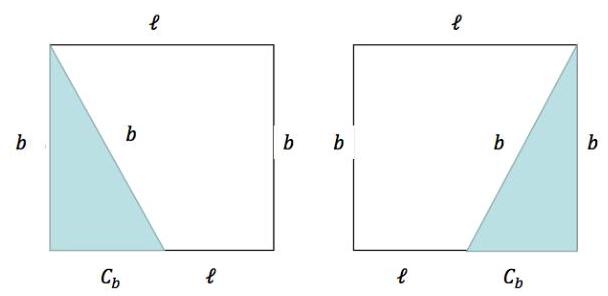
\includegraphics[max width=0.5\textwidth]{images/bo_d2bcsrref24c73avs720_117_655_468_608_296_0.jpg}
\end{center}
\hspace*{3em} 

4. Inverse: the inverse of \(\left\lbrack  u\right\rbrack\) , where \(u\) is a loop, should be \(\left\lbrack  {u}^{\prime }\right\rbrack\) , where \({u}^{\prime }\) is the reverse of the traveling of \(u\) . Therefore, for all \(u : I \rightarrow  X\) (loop based at \(b\) ), define \({u}^{-1} : I \rightarrow  X\) by \({u}^{-1}\left( t\right)  = u\left( {1 - t}\right)\) . Note that

\[
\left\lbrack  u\right\rbrack   * \left\lbrack  {u}^{-1}\right\rbrack   = \left\lbrack  {u \cdot  {u}^{-1}}\right\rbrack  ,\;e = \left\lbrack  {c}_{b}\right\rbrack
\]

It suffices to show \(u \cdot  {u}^{-1} \simeq  {c}_{b}\) and \({u}^{-1} \cdot  u \simeq  {c}_{b}\) :

The homotopy below gives \(u \cdot  {u}^{-1} \simeq  {c}_{b}\) , and the \({u}^{-1} \cdot  u \simeq  {c}_{b}\) follows similarly.

\[
H\left( {t,s}\right)  = \left\{  \begin{array}{rr} u\left( {{2t}\left( {1 - s}\right) }\right) , & 0 \leq  t \leq  1/2 \\  u\left( {\left( {2 - {2t}}\right) \left( {1 - s}\right) }\right) , & 1/2 \leq  t \leq  1 \end{array}\right.
\]

The graphic illustration is given below:

\begin{center}
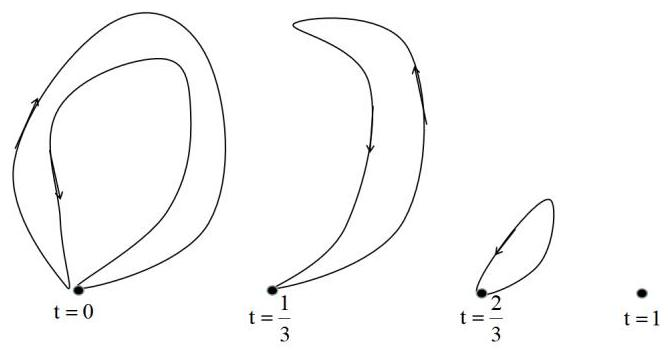
\includegraphics[max width=0.5\textwidth]{images/bo_d2bcsrref24c73avs720_117_636_1629_668_351_0.jpg}
\end{center}
\hspace*{3em} 

Note that the figure below does not define a homotopy from \(u \cdot  {u}^{-1}\) to \({c}_{b}\) !

\begin{center}
\includegraphics[max width=0.5\textwidth]{images/bo_d2bcsrref24c73avs720_118_529_423_599_389_0.jpg}
\end{center}
\hspace*{3em} 

The reason is that for the upper part, as \(s \rightarrow  1\) , the time for traveling \(u\) and \({u}^{-1}\) becomes very small, i.e., a particle has to pass \(u\) and \({u}^{-1}\) in infinitely small time, which is not well-defined.

\begin{itemize}
\item Example 11.11 The reason why \({\pi }_{1}\left( {{\mathbb{R}}^{2},b}\right)  = \{ e\}\) is trivial:
\end{itemize}

\begin{itemize}
\item For any \(u : I \rightarrow  {\mathbb{R}}^{2}\) with \(u\left( 0\right)  = u\left( 1\right)  = b\) , consider the homotopy
\end{itemize}

\[
H\left( {t,s}\right)  = \left( {1 - s}\right) u\left( t\right)  + {sb}.
\]

Therefore, \(u \simeq  {c}_{b}\) for any loop \(u\) based at \(b\) . Check the diagram below for graphic illustration of this homotopy.

\begin{center}
\includegraphics[max width=0.2\textwidth]{images/bo_d2bcsrref24c73avs720_118_659_1622_339_309_0.jpg}
\end{center}
\hspace*{3em} 

More generally, if \(X \simeq  \{ x\}\) is contractible, then \({\pi }_{1}\left( {X,b}\right)  = \{ e\}\) . The same argument cannot work for \(\left( {{\mathbb{R}}^{2}\{ 0\} ,\mathbf{b}}\right)\) , since the mapping \(H : {\mathbb{R}}^{2} \smallsetminus  \{ 0\}  \times  I \rightarrow  {\mathbb{R}}^{2} \smallsetminus  \{ 0\}\) with

\(H\left( {\mathbf{t},s}\right)  = \left( {1 - s}\right) u\left( \mathbf{t}\right)  + s\mathbf{b}\) is not well-defined. In particular, the value \(H\left( {s,t}\right)\) may hit the origin0.

However, \({\pi }_{1}\left( {{S}^{1},1}\right)\) is non-trivial. We cannot deform the loop in \({S}^{1}\) into a constant loop. We will see that \({\pi }_{1}\left( {{S}^{1},1}\right)  \cong  \mathbb{Z}\) .

Proposition 11.14 If \(b,{b}^{\prime }\) are path-connected in \(X\) , then \({\pi }_{1}\left( {X,b}\right)  \cong  {\pi }_{1}\left( {X,{b}^{\prime }}\right)\) .

Proof. Let \(w\) be a path from \(b\) to \({b}^{\prime }\) , and define

\[
{w}_{\# } : \;{\pi }_{1}\left( {X,b}\right)  \rightarrow  {\pi }_{1}\left( {X,{b}^{\prime }}\right)
\]

\[
\text{ with }\left\lbrack  \ell \right\rbrack   \mapsto  \left\lbrack  {{w}^{-1}\ell w}\right\rbrack
\]

1. Well-definedness: Check that \(\ell  \simeq  {\ell }^{\prime }\) implies \({w}^{-1}\ell w \simeq  {w}^{-1}{\ell }^{\prime }w\) . See the figure below for graphic illustration.

\begin{center}
\includegraphics[max width=0.4\textwidth]{images/bo_d2bcsrref24c73avs720_119_683_1166_568_270_0.jpg}
\end{center}
\hspace*{3em} 

2. \({w}_{\# }\) is a homomorphism:

\[
{w}_{\# }\left( \left\lbrack  {\ell }_{1}\right\rbrack  \right)  \cdot  {w}_{\# }\left( \left\lbrack  {\ell }_{2}\right\rbrack  \right)  = \left\lbrack  {{w}^{-1} \cdot  {\ell }_{1}w}\right\rbrack   \cdot  \left\lbrack  {{w}^{-1} \cdot  {\ell }_{2}w}\right\rbrack   \tag{11.4a}
\]

\[
= \left\lbrack  {{w}^{-1} \cdot  {\ell }_{1}{\ell }_{2}w}\right\rbrack   \tag{11.4b}
\]

\[
= {w}_{\# }\left( \left\lbrack  {{\ell }_{1}{\ell }_{2}}\right\rbrack  \right)  \tag{11.4c}
\]

where (11.4b) is because that \(w \cdot  {w}^{-1} = {c}_{b}\) .

3. And \({w}_{\# }\) is also injective. If loops \({\ell }_{1},{\ell }_{2}\) are such that \({w}_{\# }\left( {\ell }_{1}\right)  = {w}_{\# }\left( {\ell }_{2}\right)\) , then

\[
\left\lbrack  {{w}^{-1}{\ell }_{1}w}\right\rbrack   = \left\lbrack  {{w}^{-1}{\ell }_{2}w}\right\rbrack
\]

which follows that

\[
\left\lbrack  {\ell }_{1}\right\rbrack   = \left\lbrack  w\right\rbrack  \left\lbrack  {{w}^{-1}{\ell }_{1}w}\right\rbrack  \left\lbrack  {w}^{-1}\right\rbrack   = \left\lbrack  w\right\rbrack  \left\lbrack  {{w}^{-1}{\ell }_{2}w}\right\rbrack  \left\lbrack  {w}^{-1}\right\rbrack   = \left\lbrack  {\ell }_{2}\right\rbrack   \tag{11.5}
\]

4. Finally, \({w}_{\# }\) is surjective, because for any \(u \in  {\pi }_{1}\left( {X,{b}^{\prime }}\right)\) , let \(v = {wu}{w}^{-1}\) , then \(v\) is based at \(b\) , so \(\left\lbrack  v\right\rbrack   \in  {\pi }_{1}\left( {X,b}\right)\) , and \({w}_{\# }\left( v\right)  = \left\lbrack  u\right\rbrack\) . Therefore \({w}_{\# }\) is surjective.

In conclusion, \({w}_{\# }\) is a group isomorphism between \({\pi }_{1}\left( {X,b}\right)\) and \({\pi }_{1}\left( {X,{b}^{\prime }}\right)\) .

In (11.5) we extended the meaning of \(\left\lbrack  \ell \right\rbrack\) to allow \(\ell\) to be a path, and the equivalence class is defined by the relation " \(\sim\) ": \({\ell }_{1} \sim  {\ell }_{2}\) iff they are homotopic relative to \(\{ 0,1\}\) . The multiplication rules are defined similarly.

\section*{12.3. Monday for MAT4002}

Proposition 12.3 If \(b,{b}^{\prime }\) are path connected in \(X\) , then

\[
{\pi }_{1}\left( {X,b}\right)  \cong  {\pi }_{1}\left( {X,{b}^{\prime }}\right)
\]

R Last lecture we have given the isomorphism

\[
{W}_{\# } : \;{\pi }_{1}\left( {X,b}\right)  \rightarrow  {\pi }_{1}\left( {X,{b}^{\prime }}\right)
\]

\[
\text{ with }\left\lbrack  \ell \right\rbrack   \mapsto  \left\lbrack  {{w}^{-1} \cdot  \ell  \cdot  w}\right\rbrack
\]

where \(w\) denotes a path from \(b\) to \({b}^{\prime }\) . The inverse of \({W}_{\# }\) is given by:

\[
{W}_{\# }^{-1} : \;{\pi }_{1}\left( {X,{b}^{\prime }}\right)  \rightarrow  {\pi }_{1}\left( {X,b}\right)
\]

\[
\text{ with }\left\lbrack  m\right\rbrack   \mapsto  \left\lbrack  {w \cdot  m \cdot  {w}^{-1}}\right\rbrack
\]

Notation. For path connected space \(X\) , we will just write \({\pi }_{1}\left( X\right)\) instead of \({\pi }_{1}\left( {X,x}\right)\) .

Proposition 12.4 Let(X, x)and(Y, y)be spaces with basepoints \(x\) and \(y\) , and \(f : X \rightarrow  Y\) be a continuous map with \(f\left( x\right)  = y\) . Then every loop \(\ell  : I \rightarrow  X\) based at \(x\) gives a loop \(f \circ  \ell  : I \rightarrow  Y\) based at \(y\) , i.e., the continous map \(f\) induces a homomorphism of groups

\[
{f}_{ * } : \;{\pi }_{1}\left( {\pi ,x}\right)  \rightarrow  {\pi }_{1}\left( {Y,y}\right)
\]

\[
\left\lbrack  \ell \right\rbrack   \mapsto  \left\lbrack  {f \circ  \ell }\right\rbrack   \mathrel{\text{ := }} {f}_{ * }\left( \left\lbrack  \ell \right\rbrack  \right)
\]

Moreover,

1. \({\left( {\operatorname{id}}_{X \rightarrow  X}\right) }_{ * } = {\operatorname{id}}_{{\pi }_{1}\left( {X,x}\right)  \rightarrow  {\pi }_{1}\left( {X,x}\right) }\)

2. \({\left( g \circ  f\right) }_{ * } = {g}_{ * } \circ  {f}_{ * }\)

3. If \(f \simeq  {f}^{\prime }\) relative to \(x \in  X\) , then \({f}_{ * } = {\left( {f}^{\prime }\right) }_{ * }\)

Proof. - Well-definedness: Suppose that \(\ell  \simeq  {\ell }^{\prime }\) , then \(f \circ  \ell  \simeq  f \circ  {\ell }^{\prime }\) by propositon (9.4).

Therefore, \(\left\lbrack  {f \circ  \ell }\right\rbrack   = \left\lbrack  {f \circ  {\ell }^{\prime }}\right\rbrack\) .

\begin{itemize}
\item Homomorphism: It's clear that
\end{itemize}

\[
f \circ  \left( {\ell  \circ  {\ell }^{\prime }}\right)  = \left( {f \circ  \ell }\right)  \circ  \left( {f \circ  {\ell }^{\prime }}\right)
\]

Therefore, \({f}_{ * }\left\lbrack  {\ell {\ell }^{\prime }}\right\rbrack   = \left( {{f}_{ * }\left\lbrack  \ell \right\rbrack  }\right)  * \left( {{f}_{ * }\left\lbrack  {\ell }^{\prime }\right\rbrack  }\right)\)

The other three statements are obvious.

Proposition 12.5 Let \(X,Y\) be path-connected such that \(X \simeq  Y\) (i.e., there exists \(f : X \rightarrow  Y\) and \(g : Y \rightarrow  X\) such that \(g \circ  f \simeq  {\operatorname{id}}_{X},f \circ  g \simeq  {\operatorname{id}}_{Y}\) ). Then \({\pi }_{1}\left( X\right)  \cong  {\pi }_{1}\left( Y\right)\) .

In particular, if \(X,Y\) are path-connected with \(X \cong  Y\) , then \({\pi }_{1}\left( X\right)  \cong  {\pi }_{1}\left( Y\right)\)

Proof. Consider the mapping

\[
{\pi }_{1}\left( {X,{x}_{0}}\right) \overset{{f}_{ * }}{ \rightarrow  }{\pi }_{1}\left( {Y,{y}_{0}}\right) \overset{{g}_{ * }}{ \rightarrow  }{\pi }_{1}\left( {X,{x}_{1}}\right)
\]

It suffices to show that \({f}_{ * }\) and \({g}_{ * }\) are bijective. (The homomorphism follows from proposition (12.4))

\begin{itemize}
\item Wrong proof: \(g \circ  f \simeq  {\operatorname{id}}_{X}\) implies \({\left( g \circ  f\right) }_{ * } = {\left( {\operatorname{id}}_{X}\right) }_{ * }\) implies \({g}_{ * } \circ  {f}_{ * } = {\operatorname{id}}_{{\pi }_{1}\left( {X,{x}_{0}}\right) }\) .
\end{itemize}

Reason: note that \(\left( {g \circ  f}\right)  \simeq  {\operatorname{id}}_{X}\) is not relative to \({x}_{0}\) .

Consider the homotopy \(H : g \circ  f \simeq  {\mathrm{{id}}}_{X}\) , where \(H\left( {{x}_{0},s}\right)\) is not necessarily a constant for \(s \in  I\) . It follows that \(H\left( {{x}_{0},0}\right)  = {x}_{1}\) and \(H\left( {{x}_{0},1}\right)  = {x}_{0}\) , i.e., \(w\left( s\right)  \mathrel{\text{ := }} H\left( {{x}_{0},s}\right)\) defines a path from \({x}_{1}\) to \({x}_{0}\) .

For any loop \(\ell  : I \rightarrow  X\) based at \({x}_{0}\) , consider the homotopy

\[
K = H \circ  \left( {\ell  \times  {\operatorname{id}}_{I}}\right)  : \;I \times  I \rightarrow  X
\]

\[
K\left( {t,s}\right)  = H\left( \left( {\ell \left( t\right) ,s}\right) \right)
\]

\[
K\left( {t,0}\right)  = H\left( {\ell \left( t\right) ,0}\right)  = g \circ  f\left( {\ell \left( t\right) }\right)
\]

\[
K\left( {t,1}\right)  = H\left( {\ell \left( t\right) ,1}\right)  = \ell \left( t\right)
\]

\[
K\left( {0,s}\right)  = w\left( s\right)  = K\left( {1,s}\right)
\]

The graphic plot of \(K\) is given in the figure below:

\begin{center}
\includegraphics[max width=0.4\textwidth]{images/bo_d2bcsrref24c73avs720_123_558_340_483_462_0.jpg}
\end{center}
\hspace*{3em} 

The homotopy between \(\ell\) and \(g \circ  f \circ  \ell\) motivates us to construct a homotopy between \(\ell\) and \({w}^{-1} \circ  g \circ  f \circ  \ell  \circ  w\) relative to \(\{ 0,1\}\) :

\begin{center}
\includegraphics[max width=0.3\textwidth]{images/bo_d2bcsrref24c73avs720_123_631_1071_449_410_0.jpg}
\end{center}
\hspace*{3em} 

Therefore,

\[
\left\lbrack  \ell \right\rbrack   = \left\lbrack  {{w}^{-1}{gf}\ell w}\right\rbrack   = {W}_{\# }\left( \left\lbrack  {{gf}\ell }\right\rbrack  \right)  = \left( {{W}_{\# } \circ  {g}_{ * } \circ  {f}_{ * }}\right) \left\lbrack  \ell \right\rbrack
\]

which follows that \({W}_{\# } \circ  {g}_{ * } \circ  {f}_{ * } = {\operatorname{id}}_{{\pi }_{1}\left( {X,{x}_{0}}\right) }\) . Therfore, \({f}_{ * }\) is injective, \({g}_{ * }\) is surjective.

The similar argument gives

\[
{W}_{\# } \circ  {f}_{ * } \circ  {g}_{ * } = {\operatorname{id}}_{{\pi }_{1}\left( {Y,{y}_{0}}\right) }
\]

Therefore, \({f}_{ * }\) is surjective, \({g}_{ * }\) is injective. The bijectivity is shown.

Definition 12.1 [Simply-Connected] A space \(X\) is simply-connected if \(X\) is path connected, and \(X\) has trivial fundamental group, i.e., \({\pi }_{1}\left( X\right)  = \{ e\}\) for some point \(e \in  X\) .

\begin{itemize}
\item Example 12.4 If \(X\) is contractible, then \(X\) is path-connected. By proposition (12.5), since \(X \simeq  \{ e\}\) , we imply
\end{itemize}

\[
{\pi }_{1}\left( X\right)  \cong  {\pi }_{1}\left( {\{ e\} }\right)  = \{ e\} .
\]

Therefore, all contractible spaces (e.g., \({\mathbb{R}}^{n}\) ) are simply-connected.

However, not all simply-connected spaces are contractible, e.g., \({\pi }_{1}\left( {S}^{2}\right)  \cong  \{ e\}\) , but \({S}^{2}\) is not homotopy equivalent to a point.
\chapter{Calculations of $\pi_1(X)$}
In this chapter, we will calculate the fundamental group of various topological spaces.

More explicitly, we begin with a simplicial complex $K$ and its topological realization $X = |K|$. For $b \in X$, we will study \({\pi }_{1}\left( {X,b}\right)\) by the combinatorial structure of $K$.

\begin{definition} [Edge Loop] Let \(K = \left( {V,\Sigma }\right)\) be a simplicial complex.

\begin{enumerate}
    \item An edge path \(\left( {{v}_{0},\ldots,{v}_{n}}\right)\) is such that

(a) \({a}_{i} \in  V\left( K\right)\)

(b) For each \(i,\left\{  {{a}_{i - 1},{a}_{i}}\right\}\) spans a simplex of \(K\)

\item An edge loop is an edge path with \({a}_{n} = {a}_{0}\).

\item Let \(\alpha  = \left( {{v}_{0},\ldots,{v}_{n}}\right),\beta  = \left( {{w}_{0},\ldots,{w}_{m}}\right)\) be two edge paths with \({v}_{n} = {w}_{0}\), then we define
\[
\alpha  \circ  \beta  = \left( {{v}_{0},\ldots,{v}_{n},{w}_{1},\ldots,{w}_{m}}\right)
\]
\end{enumerate}
\end{definition}

\begin{definition} [Elementary Contraction/Expansion] Let \(\alpha,\beta\) be two edge paths.

 \begin{enumerate}
     \item An elementary contraction of \(\alpha\) is a new edge path obtained by performing one of the following on \(\alpha\):

\begin{itemize}
\item Replacing \(\cdots {a}_{i - 1}{a}_{i}\cdots\) by \(\cdots {a}_{i - 1}\cdots\) provided that \({a}_{i - 1} = {a}_{i}\)

\item Replacing \(\cdots {a}_{i - 1}{a}_{i}{a}_{i + 1}\cdots\) by \(\cdots {a}_{i - 1}\cdots\) provided that \({a}_{i - 1} = {a}_{i + 1}\)

\item Replacing \(\cdots {a}_{i - 1}{a}_{i}{a}_{i + 1}\cdots\) by \(\cdots {a}_{i - 1}{a}_{i + 1}\cdots\) provided that \(\left\{  {{a}_{i - 1},{a}_{i},{a}_{i + 1}}\right\}\) spans a 2-simplex of \(K\).
\end{itemize}

\item An elementary expansion is the reverse of the elementary contraction.

\item Two edge paths \(\alpha,\beta\) are equivalent if \(\alpha\) and \(\beta\) differs by a finite sequence of elementary contractions or expansions.

\item The equivalence class of edge loops is given by:
\[
\left\lbrack  \alpha \right\rbrack   = \left\{  {{\alpha }^{\prime } \mid  {\alpha }^{\prime } \sim  \alpha,{\alpha }^{\prime }\text{ is the edge loop based at }b}\right\}
\]
\end{enumerate}
\end{definition}

Note that \({\alpha }^{\prime } \sim  \alpha\) if they differ from finitely many elementary contractions or expansions. For instance, let \(K\) in the figure below denote a triangle:
\begin{center}
\includegraphics[width=0.25\textwidth]{images/Ch8_triangle123.jpg}
\end{center}
Then the canonical form of any equivalence form \(\left\lbrack  \alpha \right\rbrack\) can be expressed as:
\[
\left\lbrack  \alpha \right\rbrack   = \left\lbrack  {{bcabc}\cdots {ab}}\right\rbrack ,
\]
where \(a,b,c \in  \{ 1,2,3\}\) are distinct.

\begin{proposition} Let 
\begin{center}
\(E\left( {K,b}\right):= \{ \left\lbrack  \alpha \right\rbrack   \mid  \alpha\) is edge loop based at \(b\}\) 
\end{center}
Then $E\left( {K,b}\right)$ is a group with multiplication
\[
\left\lbrack  \alpha \right\rbrack   * \left\lbrack  \beta \right\rbrack   = \left\lbrack  {\alpha  \cdot  \beta }\right\rbrack
\]
We call $E(K,b)$ the \emph{edge loop group based at} $b$.
\end{proposition}

\begin{proof}
1. Well-definedness: Note that by definition,
\[
\alpha  \sim  {\alpha }^{\prime },\beta  \sim  {\beta }^{\prime } \Rightarrow  \alpha  \cdot  \beta  \sim  {\alpha }^{\prime } \cdot  {\beta }^{\prime }
\]
2. Associativity is clear.

\noindent 3. The identity is \(e = \left\lbrack  b\right\rbrack\): for any edge loop \(\left\lbrack  \alpha \right\rbrack   = \left\lbrack  {b{v}_{1}\cdots b}\right\rbrack\),

\[
\left\lbrack  \alpha \right\rbrack   * e = \left\lbrack  {b{v}_{1}\cdots {v}_{n}b}\right\rbrack   * \left\lbrack  b\right\rbrack
= \left\lbrack  {b{v}_{1}\cdots {v}_{n}{bb}}\right\rbrack
= \left\lbrack  {b{v}_{1}\cdots {v}_{n}b}\right\rbrack   = \left\lbrack  \alpha \right\rbrack .\]
Also, \(e * \left\lbrack  \alpha \right\rbrack   = \left\lbrack  \alpha \right\rbrack\).

\noindent 4. The inverse of any edge loop \(\left\lbrack  {b{v}_{1}\cdots {v}_{n}b}\right\rbrack\) is \(\left\lbrack  {b{v}_{n}\cdots {v}_{1}b}\right\rbrack\):
\begin{align*}
{\left\lbrack  b{v}_{1}\cdots {v}_{n}b\right\rbrack  }^{-1} * \left\lbrack  {b{v}_{1}\cdots {v}_{n}b}\right\rbrack  &= \left\lbrack  {b{v}_{n}\cdots {v}_{1}{bb}{v}_{1}\cdots {v}_{n}b}\right\rbrack
\\
&= \left\lbrack  {b{v}_{n}\cdots {v}_{1}b{v}_{1}\cdots {v}_{n}b}\right\rbrack
\\
&= \left\lbrack  {b{v}_{n}\cdots {v}_{2}{v}_{1}{v}_{2}\cdots {v}_{n}b}\right\rbrack
\\
&= \cdots
\\
&= \left\lbrack  b\right\rbrack
\end{align*}
Similarly, \(\left\lbrack  {b{v}_{1}\cdots {v}_{n}b}\right\rbrack   * {\left\lbrack  b{v}_{1}\cdots {v}_{n}b\right\rbrack  }^{-1} = \left\lbrack  b\right\rbrack\).
\end{proof}

Indeed, the edge loop group of a simplicial complex gives us a combinatorial way of studying the fundamental group of its topological realization: 
\begin{theorem} \label{thm:edge_loop_fundamental}
\(E\left( {K,b}\right)  \cong  {\pi }_{1}\left( {\left| K\right|,b}\right)\).
\end{theorem} 

This is the most difficult theorem that we have faced so far. To do so, we recall (a slight generalization of) the simplicial approximation theorem (\autoref{thm:simplicial_approx}): Suppose that \(f\): \(\left| K\right|  \rightarrow  \left| L\right|\) be such that for all \(v \in  V\left( K\right)\), there exists \(g\left( v\right)  \in  V\left( L\right)\) satisfying
\[
f\left( {{\operatorname{st}}_{K}\left( v\right) }\right)  \subseteq  {\operatorname{st}}_{L}\left( {g\left( v\right) }\right).
\]
Then there is a simplicial map
\(g: \;K \rightarrow  L
\)
with $v \mapsto  g\left( v\right)$
and \(\left| g\right|  \simeq  f\).

A generalization of the simplicial approximation theorem needed for the proof of \autoref{thm:edge_loop_fundamental} is as follows: if \(A \subseteq  K\)
and \(B \subseteq  L\) are simplicial subcomplexes, and \[f\left( \left| A\right| \right)  \subseteq  \left| B\right|,\] 
then the above \(g\) can be chosen such that 
\[{\left. g\right| }_{A}: A \rightarrow  B\] 
and the homotopy \(\left| g\right|  \simeq  f\) sends \(\left| A\right|\) to \(\left| B\right|\).

\begin{proof} For each edge loop \(\alpha  = \left( {{v}_{0},\ldots,{v}_{n}}\right)\) based at \(b\), consider the simplicial complex
\begin{center}
\includegraphics[width=0.4\textwidth]{images/Ch8_n_segments.jpg}
\end{center}
together with the simplicial map
\[
{g}_{\alpha }: \;{I}_{\left( n\right) } \rightarrow  K
\quad \text{ with }{g}_{\alpha }\left( i\right)  = {v}_{i}.
\]
Note that it is well-defined, since \(\{ i,i + 1\}  \in  \Sigma_{{I}_{\left( n\right) }}\), and \(\left\{  {{v}_{i},{v}_{i + 1}}\right\}   \in  \Sigma_{K}\).

Now construct the mapping
\begin{center}
\(\theta : \;\{ \alpha\ |\ \alpha \) edge loop based at \(b\}  \rightarrow  {\pi }_{1}\left( {K,b}\right)\)
\end{center}
by 
\[\alpha  \mapsto  \left\lbrack  \left| {g}_{\alpha }\right| \right\rbrack,\]
where \(\left| {g}_{\alpha }\right| : \left| {I}_{\left( n\right) }\right| \left( { \cong  \left\lbrack  {0,1}\right\rbrack  }\right)  \rightarrow  \left| K\right|\)
satisfies
\(\left| {g}_{\alpha }\right| \left( {i/n}\right)  = {v}_{i}\).

For example, let $K$ be given by
\begin{center}
\includegraphics[width=0.4\textwidth]{images/Ch8_edge_loop.jpg}
\end{center}
and $\alpha  = \left( \text{ bdeabcb }\right)$, then the simplicial map $g_{\alpha}: I_{(6)} \to K$
has realization given by:
\[
\left| {g}_{\alpha }\right| \left( 0\right)  = b,\left| {g}_{\alpha }\right| \left( {1/6}\right)  = d,\left| {g}_{\alpha }\right| \left( {2/6}\right)  = e,\cdots,\left| {g}_{\alpha }\right| \left( 1\right)  = b,
\]
So \(\left| {g}_{\alpha }\right|\) is a loop based at \(b\), and \(\left\lbrack  \left| {g}_{\alpha }\right| \right\rbrack   \in  {\pi }_{1}\left( {\left| K\right|,b}\right)\).

Now, suppose \(\alpha  \sim  {\alpha }^{\prime }\) be two edge loops differ by an elementary contraction, e.g.,
\[
{\alpha }^{\prime } = \left( \text{ bdebcb }\right)  \sim  \alpha  = \left( \text{ bdeabcb }\right).
\]
Then one can easily find a homotopy \(\left| {g}_{{\alpha }^{\prime }}\right|  \simeq  \left| {g}_{\alpha }\right|\) relative to \(\{ 0,1\}\). As a result, \(\left\lbrack  \left| {g}_{\alpha }\right| \right\rbrack   = \left\lbrack  \left| {g}_{{\alpha }^{\prime }}\right| \right\rbrack\), and we have a well-defined map:
\begin{center}
\(\widetilde{\theta }: \;\{\) edge loops based at \(b\}  / \sim\   := E\left( {K,b}\right)\rightarrow  {\pi }_{1}\left( {\left| K\right|,b}\right)\)
\end{center}
with \(\left\lbrack  \alpha \right\rbrack   \mapsto  \left\lbrack  \left| {g}_{\alpha }\right| \right\rbrack\).

Now we show \(\widetilde{\theta }\) {\bf is a homomorphism}, i.e.
\[
\widetilde{\theta }\left( {\left\lbrack  \alpha \right\rbrack   * \left\lbrack  \beta \right\rbrack  }\right)  = \widetilde{\theta }\left( \left\lbrack  \alpha \right\rbrack  \right) \widetilde{\theta }\left( \left\lbrack  \beta \right\rbrack  \right),
\]
which suffices to show \(\left\lbrack  \left| {g}_{\alpha  \cdot  \beta }\right| \right\rbrack   = \left\lbrack  {\left| {g}_{\alpha }\right| \left| {g}_{\beta }\right| }\right\rbrack\), i.e., \(\left| {g}_{\alpha  \cdot  \beta }\right|  \simeq  \left| {g}_{\alpha }\right| \left| {g}_{\beta }\right|\). Note that \(\left| {g}_{\alpha  \cdot  \beta }\right|\) and \(\left| {g}_{\alpha }\right| \left| {g}_{\beta }\right|\) are the same path with different "speeds", therefore, one can easily construct a homotopy between the maps.

Next, we show \(\widetilde{\theta }\) {\bf is surjective}: Let \(\ell : \left\lbrack  {0,1}\right\rbrack   \rightarrow  \left| K\right|\) be a loop based at \(b\). It suffices to find an edge loop \(\alpha\) such that \(\left\lbrack  \left| {g}_{\alpha }\right| \right\rbrack   = \left\lbrack  \ell \right\rbrack\), i.e., \(\left| {g}_{\alpha }\right|  \simeq  \ell\).

To do so, apply the simplicial approximation theorem such that there exist a large \(n\) and \(g: {I}_{\left( n\right) } \rightarrow  K\) such that \(\left| g\right|  \simeq  \ell\). Here we can choose \(g: {I}_{\left( n\right) } \rightarrow  K\) to be such that \(g\left( 0 \right)  = b =  g\left( n \right)\), and \(\left| g\right|  \simeq  \ell\) relative to \(\{ 0,1\}\). Then one can take 
\[\alpha  = \left( {g\left( 0\right),g\left( 1\right),\ldots,g\left( n\right) }\right),\] 
so that \(g\left( 0\right)  = b = g\left( n\right)\), with \({g}_{\alpha } = g\). Therefore, \(\left\lbrack  \left| {g}_{\alpha }\right| \right\rbrack   = \left\lbrack  \ell \right\rbrack\), and hence \(\widetilde{\theta }\) is surjective.

Now we show that $\overline{\theta}$ {\bf is injective}: Let \(\alpha  = \left( {{v}_{0},\ldots,{v}_{n}}\right)\) be an edge loop based at \(b\) such that \(\theta \left( \left\lbrack  \alpha \right\rbrack  \right)  = e\), i.e., \(\left| {g}_{\alpha }\right|  \simeq  {c}_{b}\). It suffices to show that \(\left\lbrack  \alpha \right\rbrack\) is the identity element of \(E\left( {K,b}\right)\).

Choose a homotopy \(H: I \times  I \rightarrow  \left| K\right|\) 
between \(\left| {g}_{\alpha }\right|  \simeq  {c}_{b}\):
\begin{center}
\includegraphics[width=0.4\textwidth]{images/Ch8_g_alpha_cb.jpg}
\end{center}
\hspace*{3em} 
Apply the simplicial approximation theorem on $H$, so that there exists a subdivision \({\left( I \times  I\right) }_{\left( r\right) }\) of \(I \times  I\) with $r \times r$ squares:
\begin{center}
\includegraphics[width=0.35\textwidth]{images/Ch8_Irr.jpg}
\end{center}
such that \(\left| {\left( I \times  I\right) }_{\left( r\right) }\right|  \cong I \times  I\) are isomorphic, and there exists a simplicial map
\[
G:{\left( I \times  I\right) }_{\left( r\right) } \rightarrow  K
\ \text{  such that }\ \left| G\right|  \simeq  H\text{. }
\]
Without loss of generality, assume that \(r\) is a sufficiently large multiple of \(n\). Then the graphic illustration of \(\left| G\right|\) is:
\begin{center}
\includegraphics[width=0.4\textwidth]{images/Ch8_bar_G.jpg}
\end{center}
\vspace{-3mm}
In particular, \(\left| G\right|\) maps \(\{ 0,1\}  \times  I\) into \(\{ b\} ;I \times  \{ 1\}\) into \(\{ b\} ;\left( {i/n,0}\right)\) into \(\left\{  {v}_{i}\right\} ,i = 0,\ldots,n\), and \(\left\lbrack  {i/n,\left( {i + 1}\right) /n}\right\rbrack\) into \(\left| \left( {{v}_{i},{v}_{i + 1}}\right) \right|,i = 0,\ldots,n - 1\).

Now look at the green line (with $\eta:=r/n$ vertices) at the bottom of $|G|$: it is the path from $v_0 = b$ to $v_1$, i.e.
$$G(0,0) = v_0 = b, \quad \dots, \quad G(0,\gamma/r) = v_1$$
and hence $G$ defines an edge path
\[
\left(G(0,0),\ G(0,\frac{1}{n}), \dots, G(0,\frac{\gamma-1}{n}),\ G(0,\frac{\gamma}{n})\right) = (b = v_0, v_0, \dots, v_0, v_1, \dots, v_1).
\]
As a result, the edge loop corresponding to the bottom edge of the square reads 
\[\left(G(0,0), G(0,\frac{1}{n}), \dots, G(0,\frac{n-1}{n}), G(0,1)\right) = \left( {b{v}_{0}\cdots {v}_{0}{v}_{1}\cdots {v}_{1}\cdots {v}_{n}\cdots {v}_{n}b}\right)\]
and clearly
\[
\beta  \sim  \left( {b{v}_{0}{v}_{1}{v}_{2}\cdots {v}_{n - 1}{v}_{n}b}\right)
\sim  \left( {b{v}_{1}{v}_{2}\cdots {v}_{n - 1}b}\right)  = \alpha, 
\]
i.e. $[\beta] = [\alpha] \in E(K,b)$. So it suffices to show \(\beta  \sim  e\) as edge loops, which can be seen by the sequence of elementary contractions and expansions:
\vspace{-2mm}
\begin{center}
\includegraphics[width=0.7\textwidth]{images/Ch8_edge_equivalence.jpg}
\end{center}
By tracing the above elementary contractions, one has \(\beta  \sim  \left( {b\cdots b}\right)  = \left( b\right)\) on the bottom left hand picture, and hence $[\beta] = e$.
\end{proof}

Note that the definition of \(E\left( {K,b}\right)\) only involves \(n\) -simplicials for \(n \leq  2\), so one has:
\begin{proposition} For any simplicial complex \(K\), consider the simplicial subcomplex \({\operatorname{Skel}}^{n}\left( K\right)  = \left( {{V}_{k},\Sigma_{K}^{n}}\right)\), where \(\Sigma_{K}^{n}\) consists of \(\sigma  \in  \Sigma_{K}\) with \(\left| \sigma \right|  \leq  n + 1\) (this is the \(n\)-skeleton of \(K\) ). Then
\[
{\pi }_{1}\left( {\left| K\right|,b}\right)  \cong  {\pi }_{1}\left( {\left| {{\operatorname{Skel}}^{2}\left( K\right) }\right|,b}\right)
\]
\end{proposition}
\begin{proof} Since \(E\left( {K,b}\right)\) only involves \(n\) -simplicials for \(n \leq  2\), we imply \(E\left( {K,b}\right)  \cong  E\left( {{\operatorname{Skel}}^{2}\left( K\right),b}\right)\).

Moreover, \({\pi }_{1}\left( {\left| K\right|,b}\right)  \cong  E\left( {K,b}\right)\) and \({\pi }_{1}\left( {\left| {{\operatorname{Skel}}^{2}\left( K\right) }\right|,b}\right)  \cong  E\left( {{\operatorname{Skel}}^{2}\left( K\right),b}\right)\). So the proof is complete.
\end{proof}

\begin{corollary} \label{cor:Sn_simply_connected} For \(n \geq  2,{\pi}_{1}\left({S}^{n}\right)\) is simply connected.
\end{corollary}

\begin{proof} Consider the simplicial complex \(K\) with
\[
V = \{ 1,2,\ldots,n + 2\},\;\Sigma  = \{ \text{ all proper subsets of }V\}
\]
It is clear that \(\left| K\right|  \cong \Delta^n \cong  {S}^{n}\), and \({\operatorname{Skel}}^{2}\left( K\right)\) has

\begin{itemize}
\item \(V: \{ 1,\ldots,n + 2\}\)
\item \(\Sigma^{2}\): all subsets of \(V\) with less or equal to 3 elements.
\end{itemize}
For any edge loop \(a\) in \({\pi }_{1}\left( \left| {{\operatorname{skel}}^{2}\left( K\right) }\right| \right)\), we have
\[
a = \left( {b{v}_{0}{v}_{1}{v}_{2}\cdots {v}_{n}}\right)
\sim  \left( {b{v}_{1}{v}_{2}\cdots {v}_{n - 2}{v}_{n - 1}b}\right)
\sim \dots \sim  \left( b\right)
\]
Therefore, all edge loops \(\alpha\) in \({\pi }_{1}\left( \left| {{\operatorname{skel}}^{2}\left( K\right) }\right| \right)\) satisfies \(\left\lbrack  \alpha \right\rbrack   = \left\lbrack  \left( b\right) \right\rbrack   = e\)., i.e.,
\[
{\pi }_{1}\left( \left| {{\operatorname{skel}}^{2}\left( K\right) }\right| \right)  \cong  \{ e\}
\]
which implies \({\pi }_{1}\left( \left| K\right| \right)  \cong  {\pi }_{1}\left( \left| {{\operatorname{skel}}^{2}\left( K\right) }\right| \right)  \cong  \{ e\}\). Since \(\left| K\right|  \cong  {S}^{n}\), we have
\[
{\pi }_{1}\left( {S}^{n}\right)  \cong  {\pi }_{1}\left( \left| K\right| \right)  \cong  \{ e\}.
\]
\end{proof}

\section{Fundamental Group of $S^1$}
\autoref{cor:Sn_simply_connected} does not hold for \({S}^{1}\), since the constructed \(\Sigma^{2}\) for \({S}^{1}\) does not contain \(\{ 1,2,3\}\). Instead, we have
\begin{theorem} \({\pi }_{1}\left( {S}^{1}\right)  \cong  \mathbb{Z}\).
\end{theorem}
\begin{proof} Consider the simplicial complex \(K\) below with $|K| \cong S^1$:
\begin{center}
\includegraphics[width=0.25\textwidth]{images/Ch8_triangle.jpg}
\end{center}
It suffices to show \(E\left( {K,1}\right)  \cong  \mathbb{Z}\). Define the orientation of \(\left| K\right|\) as shown below.
\begin{center}
\includegraphics[width=0.25\textwidth]{images/Ch8_triangle_oriented.jpg}
\end{center}
We construct the isomorphism between \(E\left( {K,b}\right)\) and \(\mathbb{Z}\) directly:
\begin{center}
\(\phi : \;E\left( {K,b}\right)  \rightarrow  \mathbb{Z}\)
with \(\left\lbrack  \alpha \right\rbrack   \mapsto\) winding number of \(\alpha\)
\end{center}
where the winding number of \(\alpha\) is 
\begin{center}
number of times it traverses $(2,3)$ $-$ number of times it traverses $(3,2)$.
\end{center}
Note that:

1. The winding number for \(\left( {1{23}\cdots {123}1}\right)  = m\), where $23$ shows up for \(m\) times

2. The winding number for \(\left( {1{32}\cdots {132}1}\right)  =  - n\), where $32$ shows up for \(n\) times

3. The winding number is invariant under elementary contractions and elementary expansions, since (for instance) $(1231321) \sim (123321) \sim (1221) \sim (1)$, that is, the $32$ and $23$ `cancel out' each other.

Therefore, any edge loop \(\alpha\) based at $1$ is equivalent uniquely to one of the canonical form:
\[
\alpha  \sim  \left( {{1bc1bc}\cdots {1bc1}}\right),\;\text{ where }{bc} = {32}\text{ or 23. }
\]
and $\phi: E(K,1) \to \mathbb{Z}$ is well-defined.

To see $\phi$ is a homomorphism, consider any two edge loops \(\alpha,\beta\) based at $1$. suppose that \(\left\lbrack  \alpha \right\rbrack   = \left\lbrack  \left( {{1bc1bc}\cdots {1bc1}}\right) \right\rbrack\) and \(\left\lbrack  \beta \right\rbrack   = \left\lbrack  \left( {{1pq1pq}\cdots {1pq1}}\right) \right\rbrack\) are at their canonical forms, then
\[
\phi \left( {\left\lbrack  \alpha \right\rbrack   \cdot  \left\lbrack  \beta \right\rbrack  }\right)  = \phi \left( \left\lbrack  {\alpha  \cdot  \beta }\right\rbrack  \right)  = \left\lbrack  \left( {{1bc1bc}\cdots {1bc11pq1pq}\cdots {1pq1}}\right) \right\rbrack
\]
Then one can easily check that
$\phi \left( {\left\lbrack  \alpha \right\rbrack   \cdot  \left\lbrack  \beta \right\rbrack  }\right) = \phi \left( {\left\lbrack  \alpha \right\rbrack  }\right) + \phi \left(  \left\lbrack  \beta \right\rbrack  \right)$.
Moreover, it is easy to see that $\phi$ is bijective. 
Therefore, \(\phi\) is an isomorphism.
\end{proof}

Actually, we can show that the loop based at 1 given by:
\[
\ell \;I \rightarrow  {S}^{1}
\text{ with }t \mapsto  {e}^{2\pi it}
\]
is a generator for \({\pi }_{1}\left( {{S}^{1},1}\right)\).



\begin{corollary} [Fundamental Theorem of Algebra] All non-constant polynomials in \(\mathbb{C}\) has at least one root in \(\mathbb{C}\).
\end{corollary}
\begin{proof} Suppose on the contrary that
\[
p\left( x\right)  = {a}_{n}{x}^{n} + \cdots  + {a}_{1}x + {a}_{0} \neq  0
\]
has no complex roots, then \(p\) is a continuous mapping from \(\mathbb{C}\) to \(\mathbb{C} \smallsetminus  \{ 0\}\). 

It is clear that \(\mathbb{C} \smallsetminus  \{ 0\}  \simeq  \{ z \in \mathbb{C} \mid  \left| z\right|  = 1\}\), and therefore
\(
{\pi }_{1}\left( {\mathbb{C}\smallsetminus \{ 0\} }\right)  = {\pi }_{1}\left( {S}^{1}\right)  \cong  \mathbb{Z}.
\), and the induced homomorphism \({p}_*\) of \(p\) is given by:
\[
{p}_{ * }: \;{\pi }_{1}\left( \mathbb{C}\right) \cong \{e\} \rightarrow  {\pi }_{1}\left( {\mathbb{C}\smallsetminus \{ 0\} }\right) \cong \mathbb{Z}
\]
Since $p_*$ is a group homomorphism, \({p}_{ * }\left( e\right)  = 0\).

Consider the inclusion 
$i: \;{C}_{r} \hookrightarrow  \mathbb{C}$, where \({C}_{r} = \{ z \in  \mathbb{C}\left| \right| z \mid   = r\}\) is the circle of radius $r$, and consider
the diagram given below: Or equivalently,
\begin{center}
\begin{tikzpicture}[node distance=3cm, auto]
  \node (A) {$C_r$};
  \node (B) [right of=A] {$\mathbb{C}$};
  \node (C) [below of=B] {$\mathbb{C} \setminus \{0\}$};
  \draw[->] (A) to node {$i$} (B);
  \draw[->,thick] (A) to node [swap] {$p|_{C_r}$} (C);
  \draw[->] (B) to node {$p$} (C);
\end{tikzpicture}
\end{center}
As a result, the induced homomorphism \({i}_{ * }\) of \(i\) satisfies the diagram

\begin{center}
\begin{tikzpicture}[node distance=3cm, auto]
  \node (A) {$\pi_1(C_r) \cong \mathbb{Z}$};
  \node (B) [right of=A] {$\pi_1(\mathbb{C}) \cong \{e\}$};
  \node (C) [below of=B] {$\pi_1(\mathbb{C} \setminus \{0\}) \cong \mathbb{Z}$};
  \draw[->] (A) to node {$i_*$} (B);
  \draw[->,thick] (A) to node [swap] {$(p|_{C_r})_*$} (C);
  \draw[->] (B) to node {$p_*$} (C);
\end{tikzpicture}
\end{center}
Therefore, \({p}_{ * } \circ  {i}_{ * }\) is a zero map since \({p}_{ * }\left( e\right)  = 0\), i.e., \({\left( {\left. p\right| }_{{C}_{r}}\right) }_{ * }\) is a zero homomorphism.

Now study \({\left. p\right| }_{{C}_{r}}: {C}_{r} \rightarrow  \mathbb{C} \smallsetminus  \{ 0\}\). Construct
\[ q\left( z\right)  = k \cdot  {z}^{n},\ \text{ where } k \mathrel{\text{:= }} \frac{p\left( r\right) }{{r}^{n}}
\]
Then \({\left. p\right| }_{{C}_{r}},{\left. q\right| }_{{C}_{r}}: {C}_{r} \rightarrow  \mathbb{C} \smallsetminus  \{ 0\}\) with \(p\left( r\right)  = q\left( r\right)\).

We {\bf claim} that \({\left. p\right| }_{{C}_{r}} \simeq  {\left. q\right| }_{{C}_{r}}\) for large \(r\): First construct the mapping
\[
H: \;{C}_{r} \times  \left\lbrack  {0,1}\right\rbrack   \rightarrow  \mathbb{C}
\ \text{ with }H\left( {z,t}\right)  = {tp}\left( z\right)  + \left( {1 - t}\right) q\left( z\right)
\]
and $H\left( {z,0}\right)  = q\left( z\right),H\left( {z,1}\right)  = p\left( z\right)$. 
If 
\[H: {C}_{r} \times  \left\lbrack  {0,1}\right\rbrack   \rightarrow  \mathbb{C} \smallsetminus  \{ 0\}\]
i.e. $H(z,t) \neq 0$ for all $z \in C_r$ and $t \in [0,1]$, \(H\) defines a homotopy between \({\left. p\right| }_{{C}_{r}}\) and \({\left. q\right| }_{{C}_{r}}\).

Suppose on the contrary that there exists $(z, t)$ such that
\[
\left( {1 - t}\right) p\left( z\right)  + {tq}\left( z\right)  = 0,\;\left| z\right|  = r,t \in  \left\lbrack  {0,1}\right\rbrack
\]
Or equivalently,
\[
\left( {1 - t}\right) \left( {{a}_{n}{z}^{n} + \cdots  + {a}_{1}z + {a}_{0}}\right)  + t \cdot  k{z}^{n} = 0.
\]
Substituting \(k\) with \(p\left( r\right) /{r}^{n}\) gives

\[
{a}_{n}{z}^{n} + \cdots  + {a}_{1}z + {a}_{0} = t\left( {{a}_{n - 1}{z}^{n - 1} + \cdots  + {a}_{0} - {a}_{n - 1}\frac{{z}^{n}}{r} - \cdots  - {a}_{1}\frac{{z}^{n}}{{r}^{n - 1}} - {a}_{0}\frac{{z}^{n}}{{r}^{n}}}\right)
\]

The LHS has leading order \(n\), while the RHS has leading order less or equal to \(n - 1\). As \(r = \left| z\right|  \rightarrow  \infty,t \rightarrow  \infty\). Therefore, the equality does not hold in the range \(t \in  \left\lbrack  {0,1}\right\rbrack\) when \(r\) is sufficiently large, and the claim is proved for $r$ sufficiently large.

Therefore, \({\left. p\right| }_{{C}_{r}} \simeq  {\left. q\right| }_{{C}_{r}}\) and \({\left( {\left. p\right| }_{{C}_{r}}\right) }_{ * } = {\left( {\left. q\right| }_{{C}_{r}}\right) }_{ * }\). 

Consider the induced mapping \({\left( {\left. q\right| }_{{C}_{r}}\right) }_{ * }: \mathbb{Z} \rightarrow  \mathbb{Z}\). In particular, we check the value of \({\left( {\left. q\right| }_{{C}_{r}}\right) }_{ * }\left( 1\right)\), where 1 is the generator in \({\pi }_{1}\left( {C}_{r}\right)\).

Recall that the loop
\(\ell : \;I \rightarrow  {C}_{r}
\)
with \(\ell \left( t\right)  = r{e}^{2\pi it}
\) is a generator of $\pi_1(C_r) \cong \mathbb{Z}$, i.e. \(\left\lbrack  \ell \right\rbrack   = 1\). It follows that
\[
{\left( {\left. q\right| }_{{C}_{r}}\right) }_{ * }\left( 1\right)  = {\left( {\left. q\right| }_{{C}_{r}}\right) }_{ * }\left( \left\lbrack  \ell \right\rbrack  \right)  = \left\lbrack  {{\left. q\right| }_{{C}_{r}}\left( \ell \right) }\right\rbrack   = q\left( {r{e}^{2\pi it}}\right)  = k \cdot  {r}^{n} \cdot  {e}^{2\pi int} \neq  0.
\]

Therefore, \({\left( {\left. q\right| }_{{C}_{r}}\right) }_{ * }: \mathbb{Z} \cong  {\pi }_{1}\left( {C}_{r}\right)  \rightarrow  {\pi }_{1}\left( {\mathbb{C}\backslash \{ 0\} }\right)  \cong\)  \(\mathbb{Z}\) is the nonzero map \(1 \mapsto  n\), contradicting the fact that \({\left( {\left. q\right| }_{{C}_{r}}\right) }_{ * } = {\left( {\left. p\right| }_{{C}_{r}}\right) }_{ * }\) is the zero homomorphism.
\end{proof}

\section{Fundamental Group of a Graph}

\begin{definition} [Graph] A graph \(T = \left( {V,E}\right)\) is defined by the following components:

\begin{itemize}
\item \(V\) is a finite or countable set, called vertex set;

\item \(E\) is a finite or countable set, called edge set;
\item A function \(\delta : E \rightarrow  V \times  V\) with \(\delta \left( e\right)  = \left( {\ell \left( e\right),\tau \left( e\right) }\right)\), where \(\ell \left( e\right),\tau \left( e\right)\) is known as the endpoints of \(e\).
\end{itemize}
\end{definition}

\begin{example} 1. Let \(V = \{ 1\},E = \left\{  {{e}_{1},{e}_{2},{e}_{3}}\right\}\), and define \(\delta \left( {e}_{i}\right)  = \left( {1,1}\right),i = 1,2,3\). The graph $(V, E)$ is represented below:
\begin{center}
\includegraphics[width=0.3\textwidth]{images/Ch8_3_petal.jpg}
\end{center}

2. Let \(V = \left\{  1,2,3\right\}\) and \(E = \left\{  {{e}_{1},\ldots,{e}_{6}}\right\}\), and define
\[
\delta \left( {e}_{1}\right)  = \left( {1,1}\right),\;\delta \left( {e}_{2}\right)  = \left( {1,2}\right),\;\delta \left( {e}_{3}\right)  = \left( {1,2}\right),
\delta \left( {e}_{4}\right)  = \left( {2,3}\right),\;\delta \left( {e}_{5}\right)  = \left( {2,3}\right),\;\delta \left( {e}_{6}\right)  = \left( {3,3}\right).
\]
The graph $(V, E)$ is represented below (We do not care the direction of edges for this graph):
\begin{center}
\includegraphics[width=0.5\textwidth]{images/Ch8_4_circles.jpg}
\end{center}
\end{example}

\begin{definition} [Realization of a Graph] For a given graph \(\Gamma  = \left( {V,E}\right)\), construct a realization by
\[
\{ \left| V\right|  \times  \{ \text{ zero simplices }\} \coprod \left| E\right|  \times  \{ 1\text{ -simplices } \} / \sim
\]
where the equivalence class is induced from the function \(\delta\). We still call this realization of the graph as \(\Gamma\).
\end{definition}

In general, graphs are not simplicial complexes. But we can "sub-divide" each edge of \(\Gamma\) into three parts such that there exists simplicial complex \(K\) with \(\left| K\right|  \cong  \Gamma\). For instance,
\begin{center}
\includegraphics[width=0.9\textwidth]{images/Ch8_simp_cplx.jpg}
\end{center}

\begin{definition}
Let $\Gamma = (V,E)$ be a graph:
\begin{itemize}
\item A \emph{subgraph} \({\Gamma }^{\prime } \subseteq  \Gamma\) is \({\Gamma }^{\prime } = \left( {{V}^{\prime },{E}^{\prime }}\right)\) with \({V}^{\prime } \subseteq  V\) and \({E}^{\prime } \subseteq  E\), and
\[
\delta { \mid  }_{{V}^{\prime }}: {E}^{\prime } \rightarrow  {V}^{\prime } \times  {V}^{\prime }
\]
\item An \emph{edge path} is a continuous function \(p: \left\lbrack  {0,1}\right\rbrack   \rightarrow  \Gamma\) such that there exists \(n \in  \mathbb{N}\) satisfying
\[
{\left. p\right| }_{\left\lbrack  i/n,i + 1/n\right\rbrack  }: \left\lbrack  {\frac{i}{n},\frac{i + 1}{n}}\right\rbrack   \rightarrow  T
\]
is a path along an edge of \(\Gamma\), or a constant function on a vertex of \(\Gamma\), for \(0 \leq  i \leq  n - 1\).
\end{itemize}
\end{definition}

Under the homeomorphism \(\Gamma  \cong  \left| K\right|\), each edge path is homotopic to \(\left| {g}_{\alpha }\right|\) for some edge path \(\alpha\) in the simplicial complex \(K\). For instance:
\begin{center}
\includegraphics[width=1\textwidth]{images/Ch8_edge_path_approx.jpg}
\end{center}

Here are more definitions:
\begin{definition}
Let $\Gamma = (V,E)$ be a graph:
\begin{itemize}
\item An edge loop is an edge path \(p\) such that \(p\left( 0\right)  = p\left( 1\right)  = b \in  V\).
\item An embedded edge loop is an injective edge loop, i.e., \(p: \left\lbrack  {0,1}\right\rbrack   \rightarrow  \Gamma\) such that for \(x \notin  V,\;{p}^{-1}\left( x\right)  = \varnothing\) or a single point.
\item A tree is a connected graph \(T\) that contains no embedded edge loop \(p: \left\lbrack  {0,1}\right\rbrack   \rightarrow  T\). For instance, as shown in the figure, \({T}_{1}\) contains no edge loop, in particular, the edge loop $(a, b, a)$ is not embedded; \({T}_{2}\) contains embedded edge loop $(a, b, c, d, a)$.

\item Maximal Tree of a connected graph \(\Gamma\) is a subgraph \(T\) of \(\Gamma\) such that 
\begin{itemize}
    \item \(T\) is a tree; and 
    \item By adding an edge \(e \in  E\left( \Gamma \right)  \smallsetminus  E\left( T\right)\) into \(T\), the new graph is no longer a tree.
\end{itemize}
 \end{itemize}
 \end{definition}


For instance, \(T \subseteq  \Gamma\) shown in the figure below is a maximal tree.
\begin{center}
\includegraphics[width=0.4\textwidth]{images/Ch8_maximal_tree.jpg}
\end{center}

With all the definitions given above, we can finally compute the fundamental group of a (connected) graph:
\begin{theorem} \label{thm:max_tree_exists} Let \(\Gamma\) be a connected graph, and \(T\) is a subgraph of \(\Gamma\) such that \(T\) is a tree. Then \(T\) is a maximal tree if and only if \(V\left( T\right)  = V\left( \Gamma \right)\).

Moreover, there always exists a maximal tree for all \(\Gamma\).
\end{theorem}

\begin{proof} Outline for second part: Construct an ordering of \(\left\{  {{v}_{1},\ldots,{v}_{i}}\right\}   \subseteq  V\left( \Gamma \right)\), such that for each integer \(i \geq  2\), there is an edge connecting \({v}_{i + 1}\) with some vertex in \(\left\{  {{v}_{1},\ldots,{v}_{i}}\right\}\).
Then construct 
\[{T}_{1} \subseteq  {T}_{2} \subseteq  \cdots,\] 
where \({T}_{i}\) is a tree containing vertices \(\left\{  {{v}_{1},\ldots,{v}_{i}}\right\}\). As a result, \(T = { \cup  }_{i \in  \mathbb{N}}{T}_{i}\) is a maximal tree.
\end{proof}


\begin{theorem} Let \(\Gamma\) be a connected graph. Then \(\pi \left( \Gamma \right)\) is isomorphic to the free group generated by \(\# \{ E\left( \Gamma \right)  \smallsetminus  E\left( T\right) \}\) elements, for any maximal tree of \(\Gamma\).
\end{theorem}


For instance, a maximal tree of the the graph \(T \subseteq  {\Gamma }_{1}\) is: 
\begin{center}
\includegraphics[width=0.5\textwidth]{images/Ch8_maximal_tree.jpg}
\end{center}
Therefore, \({\pi }_{1}\left( {\Gamma }_{1}\right)  \cong  \langle a,b,c,d\rangle\) since \(\# \left\{  {E\left( {\Gamma }_{1}\right)  \smallsetminus  E\left( T\right) }\right\}   = 4\).

On the other hand, a maximal tree of the graph with `4-petals' \(T \subseteq  {\Gamma }_{2}\) is just the middle vertexc:
\begin{center}
\includegraphics[width=0.3\textwidth]{images/Ch8_4_petals.jpg}
\end{center}
Therefore, \({\pi }_{1}\left( {\Gamma }_{2}\right)  \cong  \langle a,b,c,d\rangle\) since \(\# \left\{  {E\left( {\Gamma }_{2}\right)  \smallsetminus  E\left( T\right) }\right\}   = 4\).

Indeed, one has \({\Gamma }_{1} \simeq  {\Gamma }_{2}\). The reason for such homotopy equivalence is in the link

https://www.math3ma.com/blog/clever-homotopy-equivalences

\bigskip
We will not prove the theorem. Instead, we present the idea of the proof in the special case of \(\Gamma\) with the following specified maximal tree $T$ and orientation:
\begin{center}
\includegraphics[width=0.6\textwidth]{images/Ch8_maximal_tree_oriented.jpg}
\end{center}
and the simplicial complex $K$ with \(\left| K\right|  \cong  \Gamma\):
\begin{center}
\includegraphics[width=0.6\textwidth]{images/Ch8_simp_approx_oriented.jpg}
\end{center}
Now we construct the group homomorphism
\[
\phi : \;\langle \alpha,\beta,\gamma,\delta \rangle  \rightarrow  E\left( {K,b}\right)  \cong  {\pi }_{1}\left( \Gamma \right)
\]
with 
\begin{align*} \phi \left( \alpha \right)  &= \left\lbrack  {b{a}^{\prime }{a}^{\prime \prime }b}\right\rbrack\\ 
\phi \left( \beta \right)  &= \left\lbrack  {{be}{e}^{\prime }{f}^{\prime \prime }{b}^{\prime }{b}^{\prime \prime }b}\right\rbrack \\
\phi \left( \gamma \right)  &= \left\lbrack  {{be}{e}^{\prime }{f}^{\prime \prime }{f}^{\prime }{fd}{c}^{\prime }{c}^{\prime \prime }{f}^{\prime \prime }{e}^{\prime }{eb}}\right\rbrack
\\
\phi \left( \delta \right)  &= \left\lbrack  {{\text{ bee }}^{\prime }{f}^{\prime \prime }{f}^{\prime }{fd}{d}^{\prime \prime }{d}^{\prime }{df}{f}^{\prime }{f}^{\prime \prime }{e}^{\prime }{eb}}\right\rbrack
\end{align*}
We can show the group homomorphism \(\phi\) is bijective. In particular, the inverse of \(\phi\) is given by:
\[
\Psi : \;E\left( {K,b}\right)  \rightarrow  \langle \alpha,\beta,\gamma,\delta \rangle
\]
where for any \(\left\lbrack  \ell \right\rbrack   \mathrel{\text{:= }} \left\lbrack  {b{v}_{1}\cdots {v}_{n}}\right\rbrack   \in  E\left( {K,b}\right)\), the mapping \(\Psi \left\lbrack  \ell \right\rbrack\) is constructed by

(a) Remove all other letters appearing in \(\ell\) except \(b,{a}^{\prime },{a}^{\prime \prime },{b}^{\prime },{b}^{\prime \prime },{c}^{\prime },{c}^{\prime \prime },{d}^{\prime },{d}^{\prime \prime }\)

(b) Assign
\[
\alpha,{\alpha }^{-1},\beta,{\beta }^{-1},\gamma,{\gamma }^{-1},\delta,{\delta }^{-1}
\]
for each appearance of
\[
{a}^{\prime }{a}^{\prime \prime },{a}^{\prime \prime }{a}^{\prime },{b}^{\prime }{b}^{\prime \prime },{b}^{\prime \prime }{b}^{\prime },{c}^{\prime }{c}^{\prime \prime },{c}^{\prime \prime }{c}^{\prime },{d}^{\prime }{d}^{\prime \prime },{d}^{\prime \prime }{d}^{\prime }
\]
respectively.
\chapter{The Seifert-Van Kampen Theorem}
Here is the statement of Seifert-Van Kampen Theorem:
\begin{theorem} Let \(K = {K}_{1} \cup  {K}_{2}\) be the union of two path-connected open sets, where \({K}_{1} \cap  {K}_{2}\) is also path-connected. Take \(b \in  {K}_{1} \cap  {K}_{2}\), and suppose the group presentations for \({\pi }_{1}\left( {{K}_{1},b}\right),{\pi }_{1}\left( {{K}_{2},b}\right)\) are
\[
{\pi }_{1}\left( {{K}_{1},b}\right)  \cong  \left\langle  {{X}_{1} \mid  {R}_{1}}\right\rangle ,\;{\pi }_{1}\left( {{K}_{2},b}\right)  \cong  \left\langle  {{X}_{2} \mid  {R}_{2}}\right\rangle .
\]
Let the inclusions be
\[
{i}_{1} : {K}_{1} \cap  {K}_{2} \hookrightarrow  {K}_{1},\;{i}_{2} : {K}_{1} \cap  {K}_{2} \hookrightarrow  {K}_{2},
\]
then a presentation of \({\pi }_{1}\left( {K,b}\right)\) is given by:
\[
{\pi }_{1}\left( {K,b}\right)  \cong  \left\langle  {{X}_{1} \cup  {X}_{2} \mid  {R}_{1} \cup  {R}_{2} \cup  \left\{  {{\left( {i}_{1}\right) }_{ * }\left( g\right)  = {\left( {i}_{2}\right) }_{ * }\left( g\right)  : \forall g \in  {\pi }_{1}\left( {{K}_{1} \cap  {K}_{2},b}\right) }\right\}  }\right\rangle .
\]
(Here \({\left( {i}_{1}\right) }_{ * } : {\pi }_{1}\left( {{K}_{1} \cap  {K}_{2},b}\right)  \hookrightarrow  {\pi }_{1}\left( {{K}_{1},b}\right)\) and \({\left( {i}_{2}\right) }_{ * } : {\pi }_{1}\left( {{K}_{1} \cap  {K}_{2},b}\right)  \hookrightarrow  {\pi }_{1}\left( {{K}_{2},b}\right)\).)
\end{theorem}

\begin{example} Let \(K = {S}^{1} \vee  {S}^{1}\) given by
\begin{center}
\includegraphics[width=0.2\textwidth]{images/Ch9_S1vS1.jpg}
\end{center}

Let \(b\) be the intersection between two circles, and construct \({K}_{1},{K}_{2}\) as shown below: 

\begin{center}
\includegraphics[width=0.8\textwidth]{images/Ch9_K1K2_1.jpg}
\end{center}

We can see that \({K}_{1} \cap  {K}_{2}\) is contractible:
\begin{center}
\includegraphics[width=0.5\textwidth]{images/Ch9_K1capK2_1.jpg}
\end{center}
As we proved before, \({\pi }_{1}\left( {S}^{1}\right)  \cong  \mathbb{Z}\), which follows that
\[
{\pi }_{1}\left( {{K}_{1},b}\right)  \cong  \langle \alpha \rangle,\;{\pi }_{1}\left( {{K}_{2},b}\right)  \cong  \langle \beta \rangle
\]
Also, \({\pi }_{1}\left( {{K}_{1} \cap  {K}_{2},b}\right)  \cong  {\pi }_{1}\left( {\{ b\},b}\right)  \cong  \{ e\} \text{. }
\)

Also, it is easy to compute \({\left( {i}_{1}\right) }_{ * }\) and \({\left( {i}_{2}\right) }_{ * }\) : For instance, \({\left( {i}_{2}\right) }_{ * } : \;{\pi }_{1}\left( {{K}_{1} \cap  {K}_{2}}\right)  \rightarrow  {\pi }_{1}\left( {K}_{2}\right)\)
is given by $e \mapsto  e$. 
Therefore, by Seifert-Van Kampen Theorem,
\[
{\pi }_{1}\left( {K,b}\right)  \cong  \langle \alpha,\beta  \mid  e = e\rangle  \cong  \langle \alpha,\beta \rangle
\]

More generally, by induction

\[
{\pi }_{1}\left( {{ \vee  }^{n}{S}^{1},b}\right)  \cong  \left\langle  {{a}_{1},\ldots,{a}_{n}}\right\rangle
\]

For instance, the figure illustration for \({ \vee  }^{4}{S}^{1}\) and the basepoint \(b\) is given below:
\begin{center}
\includegraphics[width=0.35\textwidth]{images/Ch9_4_petals.jpg}
\end{center}
\end{example}

\begin{example}
Consider\({S}^{2} = {K}_{1} \cup  {K}_{2}\), which is shown below:
\begin{center}
\includegraphics[width=0.8\textwidth]{images/Ch9_S2_K1K2.jpg}
\end{center}
Therefore, we see that \({K}_{1} \cap  {K}_{2} \simeq  {S}^{1}\) :
\begin{center}
\includegraphics[width=0.6\textwidth]{images/Ch9_S2_K1capK2_S1.jpg}
\end{center}
while \({K}_{1}\) and \({K}_{2}\) are contractible. Therefore
\[
{\pi }_{1}\left( {K}_{1}\right)  \cong  \langle \beta  \mid  \beta \rangle,\;{\pi }_{1}\left( {K}_{2}\right)  \cong  \langle \gamma  \mid  \gamma \rangle
\]
and 
\({\pi }_{1}\left( {{K}_{1} \cap  {K}_{2}}\right)  \cong  {\pi }_{1}\left( {S}^{1}\right)  \cong  \langle \alpha \rangle\).

Now we compute \({\left( {i}_{1}\right) }_{ * }\) and \({\left( {i}_{2}\right) }_{ * }\): 
For any loop \(\gamma\) in $K_1 \cap K_2$ based at \(b\), Since \({K}_{1}\) is contractible, we imply \(\gamma\) in \({K}_{1}\) is homotopic to \({c}_{b}\), i.e.,
\[
{\left( {i}_{1}\right) }_{ * }\left( \left\lbrack  \gamma \right\rbrack  \right)  = \left\lbrack  {{i}_{1}\left( \gamma \right) }\right\rbrack   = e,\forall \gamma  \in  {\pi }_{1}\left( {{K}_{1} \cap  {K}_{2}}\right).
\]
Similarly, \({\left( {i}_{2}\right) }_{ * }\left( \left\lbrack  \gamma \right\rbrack  \right)  = e\).

Therefore, by Seifert-Van Kampen Theorem, we conclude that
\[
{\pi }_{1}\left( {S}^{2}\right)  \cong  \langle \beta,\gamma  \mid  \beta,\gamma,e = e\rangle  \cong  \{ e\}
\]
\end{example}

Homework: Use the same trick to check that \({\pi }_{1}\left( {S}^{n}\right)  = \{ e\}\) for all \(n \geq  2\) (Hint: for \({S}^{3}\), construct
\[
{K}_{1} = \left\{  {\left( {{x}_{1},\ldots,{x}_{4}}\right)  \in  {S}^{3} \mid  {x}_{4} >  - 1/2}\right\}
\]
and
\[
{K}_{1} = \left\{  {\left( {{x}_{1},\ldots,{x}_{4}}\right)  \in  {S}^{3} \mid  {x}_{4} < 1/2}\right\})
\]

\begin{example}
Consider \(K \cong  {\mathbb{T}}^{2}\), and \(K = {K}_{1} \cup  {K}_{2}\) given by:
\begin{center}
\includegraphics[width=0.6\textwidth]{images/Ch9_T_K1K2.jpg}
\end{center}
Therefore, we can see that \({K}_{1}\) is contractible, and \({K}_{2}\) is homotopy equivalent
to \({S}^{1} \vee  {S}^{1}\) :
\begin{center}
\includegraphics[width=0.6\textwidth]{images/Ch9_T_K1capK2.jpg}
\end{center}
and \({K}_{1} \cap  {K}_{2}\) is homotopic equivalent to the circle:
\begin{center}
\includegraphics[width=0.6\textwidth]{images/Ch9_T_K1capK2_2.jpg}
\end{center}
It follows that
\[
{\pi }_{1}\left( {K}_{1}\right)  \cong  \{ e\},\;{\pi }_{1}\left( {K}_{2}\right)  \cong  \langle \alpha,\beta \rangle,\ {\pi }_{1}\left( {{K}_{1} \cap  {K}_{2}}\right)  \cong  \langle \gamma \rangle.\]
Then we compute \({\left( {i}_{1}\right) }_{ * }\) and \({\left( {i}_{2}\right) }_{ * }\). Firstly, \({\left( {i}_{1}\right) }_{ * }\) is trivial as in the previous example:
\[
{\left( {i}_{1}\right) }_{ * } : \;{\pi }_{1}\left( {{K}_{1} \cap  {K}_{2}}\right)  \rightarrow  {\pi }_{1}\left( {K}_{1}\right)
\ \text{ with }\left\lbrack  \alpha \right\rbrack   \mapsto  e
\]
As for \({\left( {i}_{2}\right) }_{ * }\), let \(\gamma\) be any loop in $K_1 \cap K_2$. We draw the graph for \({i}_{2}\left( \gamma \right)\) :
\begin{center}
\includegraphics[width=0.8\textwidth]{images/Ch9_K12_into_K2.jpg}
\end{center}
Therefore,
\[
{\left( {i}_{2}\right) }_{ * }\left\lbrack  \gamma \right\rbrack   = \left\lbrack  {{i}_{2}\left( \gamma \right) }\right\rbrack   = \left\lbrack  {{\alpha \beta }{\alpha }^{-1}{\beta }^{-1}}\right\rbrack
\]
And by Seifert-Van Kampen Theorem, we conclude that
\[
{\pi }_{1}\left( K\right)  \cong  \left\langle  {\alpha,\beta  \mid  \beta,{\alpha \beta }{\alpha }^{-1}{\beta }^{-1} = e}\right\rangle   \cong  \langle \alpha,\beta  \mid ,{\alpha \beta } = {\beta \alpha }\rangle  \cong  \mathbb{Z} \times  \mathbb{Z}
\]
\end{example}

Exercise: The Klein bottle \(K\) shown in graph below satisfies \({\pi }_{1}\left( K\right)  = \left\langle  {a,b \mid  {ab}{a}^{-1}b}\right\rangle\).
\begin{center}
\includegraphics[width=0.35\textwidth]{images/Ch9_Klein.jpg}
\end{center}

\begin{example}
Consider the space \(K = \mathbb{R}{P}^{2}\) with \(K = {K}_{2} \cup  {K}_{2}\) given by:
\begin{center}
\includegraphics[width=0.7\textwidth]{images/Ch9_RP2_K1K2.jpg}
\end{center}
It is clear that \({K}_{1}\) is contractible. And in Homework 3, we can see that \({K}_{2} \simeq  {S}^{1}\). Moreover, \({K}_{1} \cap  {K}_{2} \simeq  {S}^{1}\) as before. Therefore, 
\[{\pi }_{1}\left( {K}_{1}\right)  = \{ e\},\ {\pi }_{1}\left( {K}_{2}\right)  = \langle \alpha \rangle,\ {\pi }_{1}\left( {{K}_{1} \cap  {K}_{2}}\right)  = \langle \gamma \rangle.\]
It’s easy to see that \({\left( {i}_{1}\right) }_{ * }\left( \left\lbrack  \gamma \right\rbrack  \right)  = e\) for any loop \(\gamma\). As for \({\left( {i}_{2}\right) }_{ * }\left( \left\lbrack  \gamma \right\rbrack  \right)\):
\begin{center}
\includegraphics[width=0.7\textwidth]{images/Ch9_RP2_i2star.jpg}
\end{center}
Therefore, \({\left( {i}_{2}\right) }_{ * }\left( \left\lbrack  \gamma \right\rbrack  \right)  = \left\lbrack  {{i}_{2}\left( \gamma \right) }\right\rbrack   = \left\lbrack  {\alpha }^{2}\right\rbrack\).

By Seifert-Van Kampen Theorem, we conclude that
\[
{\pi }_{1}\left( K\right)  \cong  \left\langle  {\alpha  \mid  {\alpha }^{2} = e}\right\rangle   \cong  \mathbb{Z}/2\mathbb{Z}
\]
\end{example}

\begin{example}
Let \(K = {\mathbb{R}}^{2} \smallsetminus  \{ 2\) points \(\alpha,\beta \}\). As we have shown in Homework 3, \(K \simeq  {S}^{1} \vee  {S}^{1}\), which implies
\[
{\pi }_{1}\left( K\right)  \cong  {\pi }_{1}\left( {{S}^{1} \land  {S}^{1}}\right)  \cong  \langle \alpha,\beta \rangle.
\]

We can compute the fundamental group for \(K\) using Seifert-Van Kampen Theorem directly: Construct \(K = {K}_{1} \cup  {K}_{2}\) as follows:
\begin{center}
\includegraphics[width=0.3\textwidth]{images/Ch9_lasteg_K1K2.jpg}
\end{center}
It is clear that \({K}_{1} \cong  {\mathbb{R}}^{2} \smallsetminus  \{\) one point \(\}  \simeq  {S}^{1}\) and similarly \({K}_{2} \simeq  {S}^{1}\). Moreover, \({K}_{1} \cap  {K}_{2}\) is contractible. Therefore,
\[
{\pi }_{1}\left( {K}_{1}\right)  \cong  \langle \alpha \rangle,\;{\pi }_{1}\left( {K}_{2}\right)  \cong  \langle \beta \rangle,\;{\pi }_{1}\left( {{K}_{1} \cap  {K}_{2}}\right)  \cong  \{ e\}
\]
Also, \({\left( {i}_{1}\right) }_{ * }\) and \({\left( {i}_{2}\right) }_{ * }\) is trivial, since \({\pi }_{1}\left( {{K}_{1} \cap  {K}_{2}}\right)  \cong  \{ e\}\).

By Seifert-Van Kampen Theorem, we conclude that
\[
{\pi }_{1}\left( K\right)  \cong  \langle \alpha,\beta  \mid  e = e\rangle  \cong  \langle \alpha,\beta \rangle
\]
\end{example}

\end{document}